\documentclass[xcolor={dvipsnames}]{beamer} % dvipsnames gives more built-in colors
\mode<presentation>

\usetheme{Boadilla}

\definecolor{GWdarkblue}{HTML}{033C5A}

\usecolortheme[named=GWdarkblue]{structure}

% Sets the font
\usepackage[defaultfam,tabular,lining]{montserrat}
% Capital case titles
\setbeamerfont{title}{shape=\scshape}
\setbeamerfont{frametitle}{shape=\scshape}

%Remove "Figure" from captions
\setbeamertemplate{caption}{\raggedright\insertcaption\par}

\usepackage{graphicx}
\usepackage{hyperref}
\usepackage{tabularx}
\usepackage{marvosym}

\title[Data Visualization]{Data Visualization}
\author[SMPA 2152]{Data Analysis for Journalism and Political Communication (Spring 2025)}
\date{Prof. Bell}

\begin{document}


%%%%%%%%%%%%%%%%%%%%%%%%%%%%%%%%%%%%%%%%%%%%%%%%%%%%%%%%%%%%%%%%%%
\frame{
\titlepage
}

%%%%%%%%%%%%%%%%%%%%%%%%%%%%%%%%%%%%%%%%%%%%%%%%%%%%%%%%%%%%%%%%%%
\frame{\frametitle{Michel Florent van Langren (1644)}
\centering
\only<1>{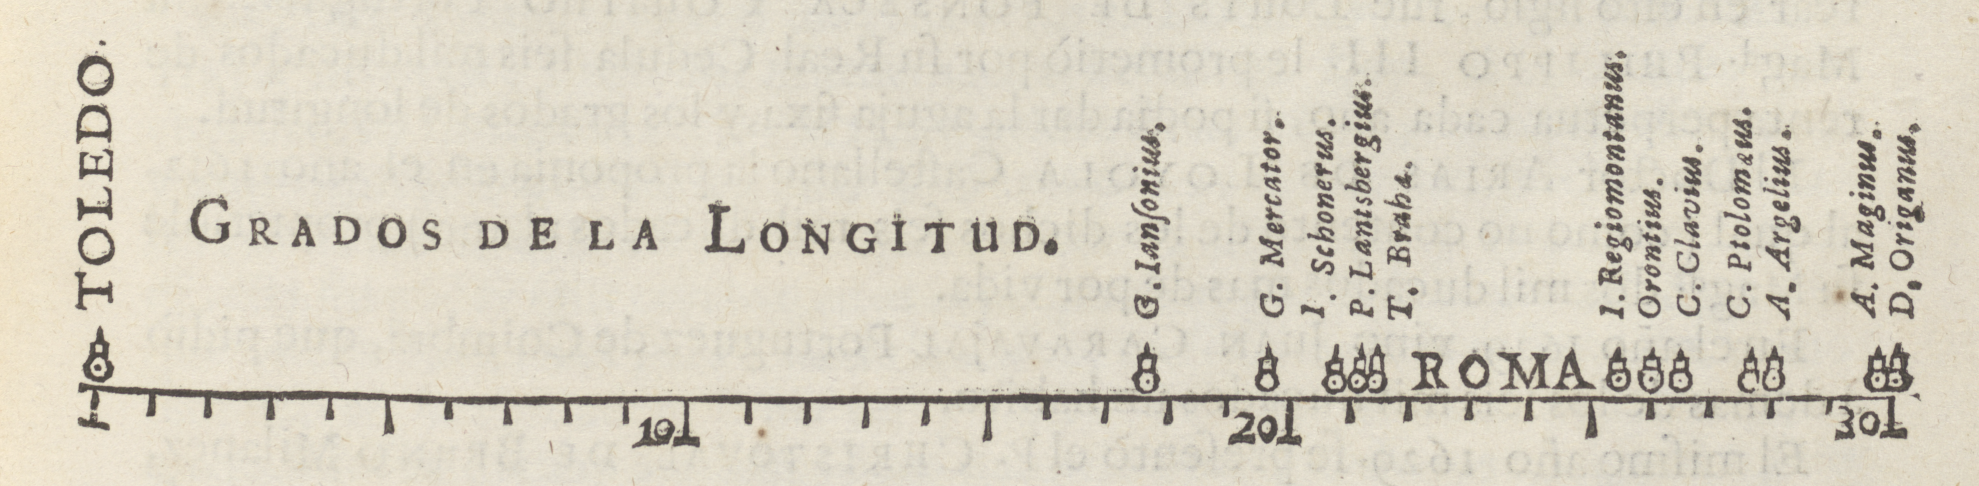
\includegraphics[width=\textheight]{florent_van_langren.png}}
\only<2>{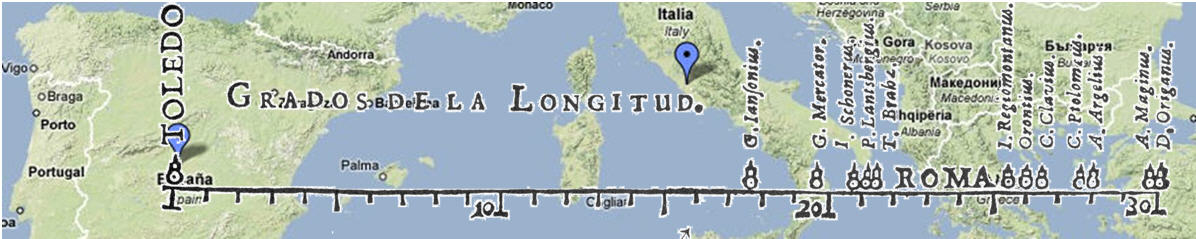
\includegraphics[width=\textheight]{florent_van_langren_overlay.jpg}}
}

%%%%%%%%%%%%%%%%%%%%%%%%%%%%%%%%%%%%%%%%%%%%%%%%%%%%%%%%%%%%%%%%%%
\frame{
\centering
\only<1>{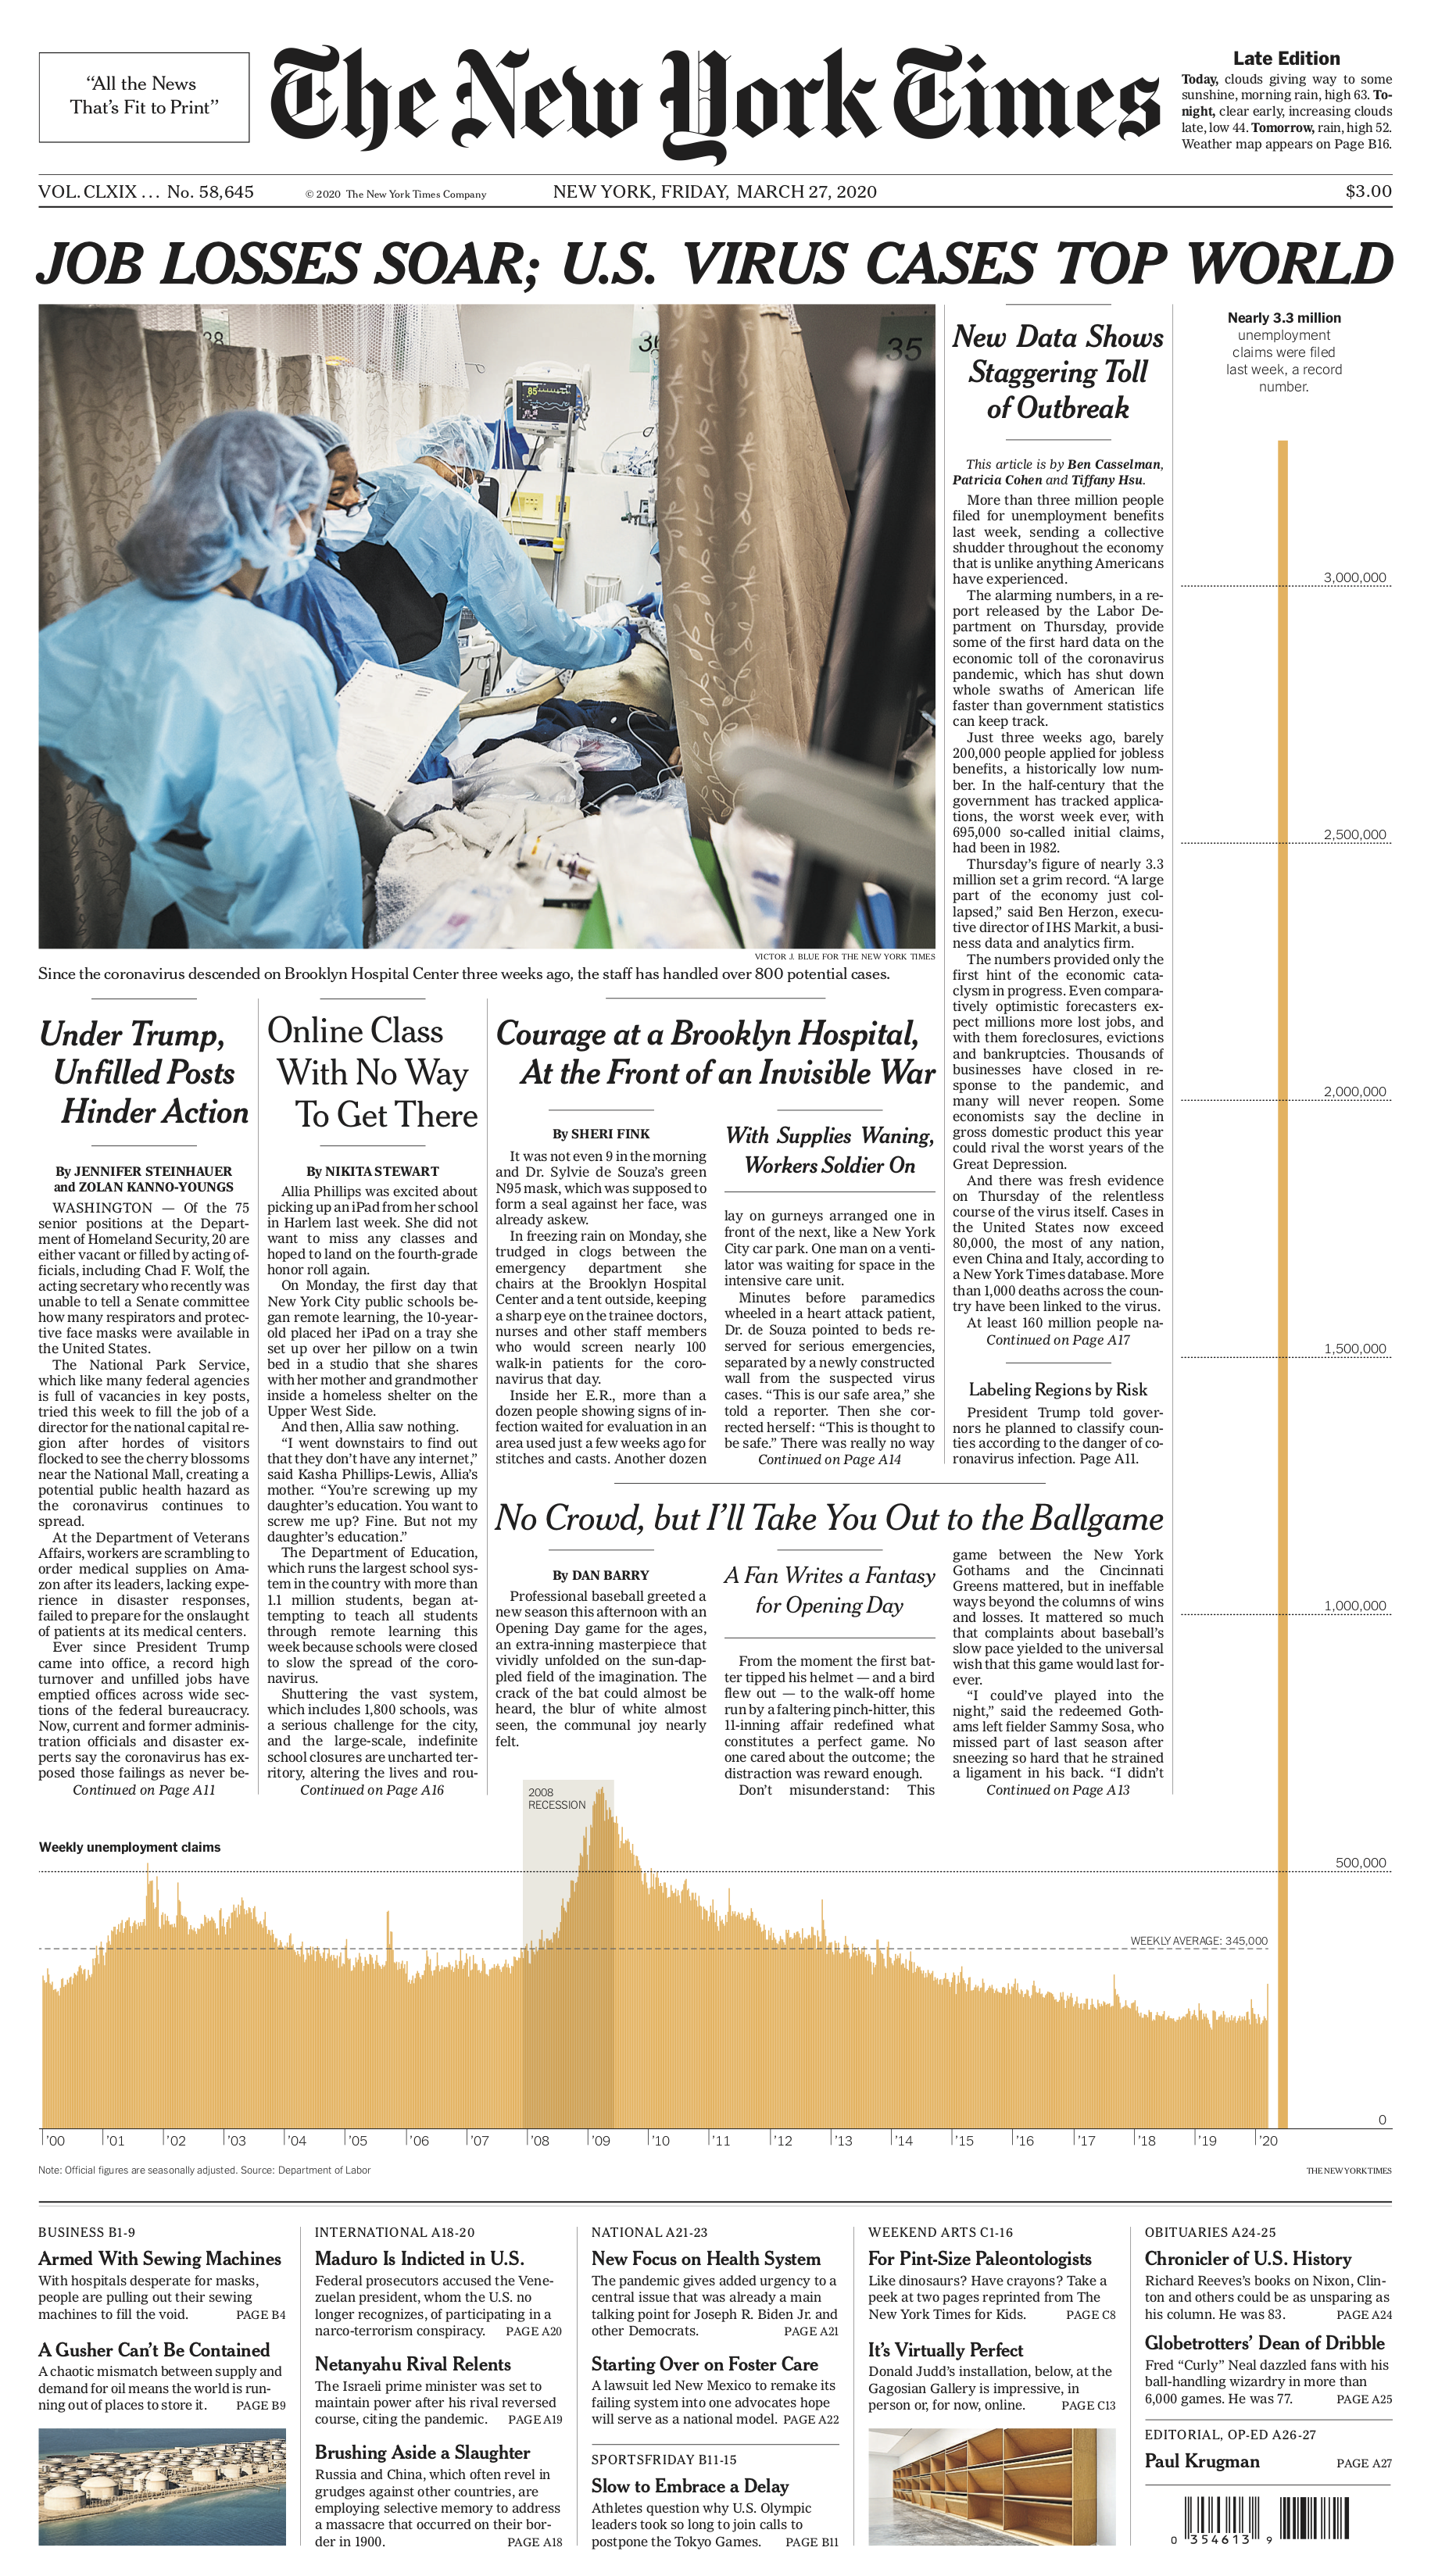
\includegraphics[height=.9\textheight]{nyt_unemp.png}}
\only<2>{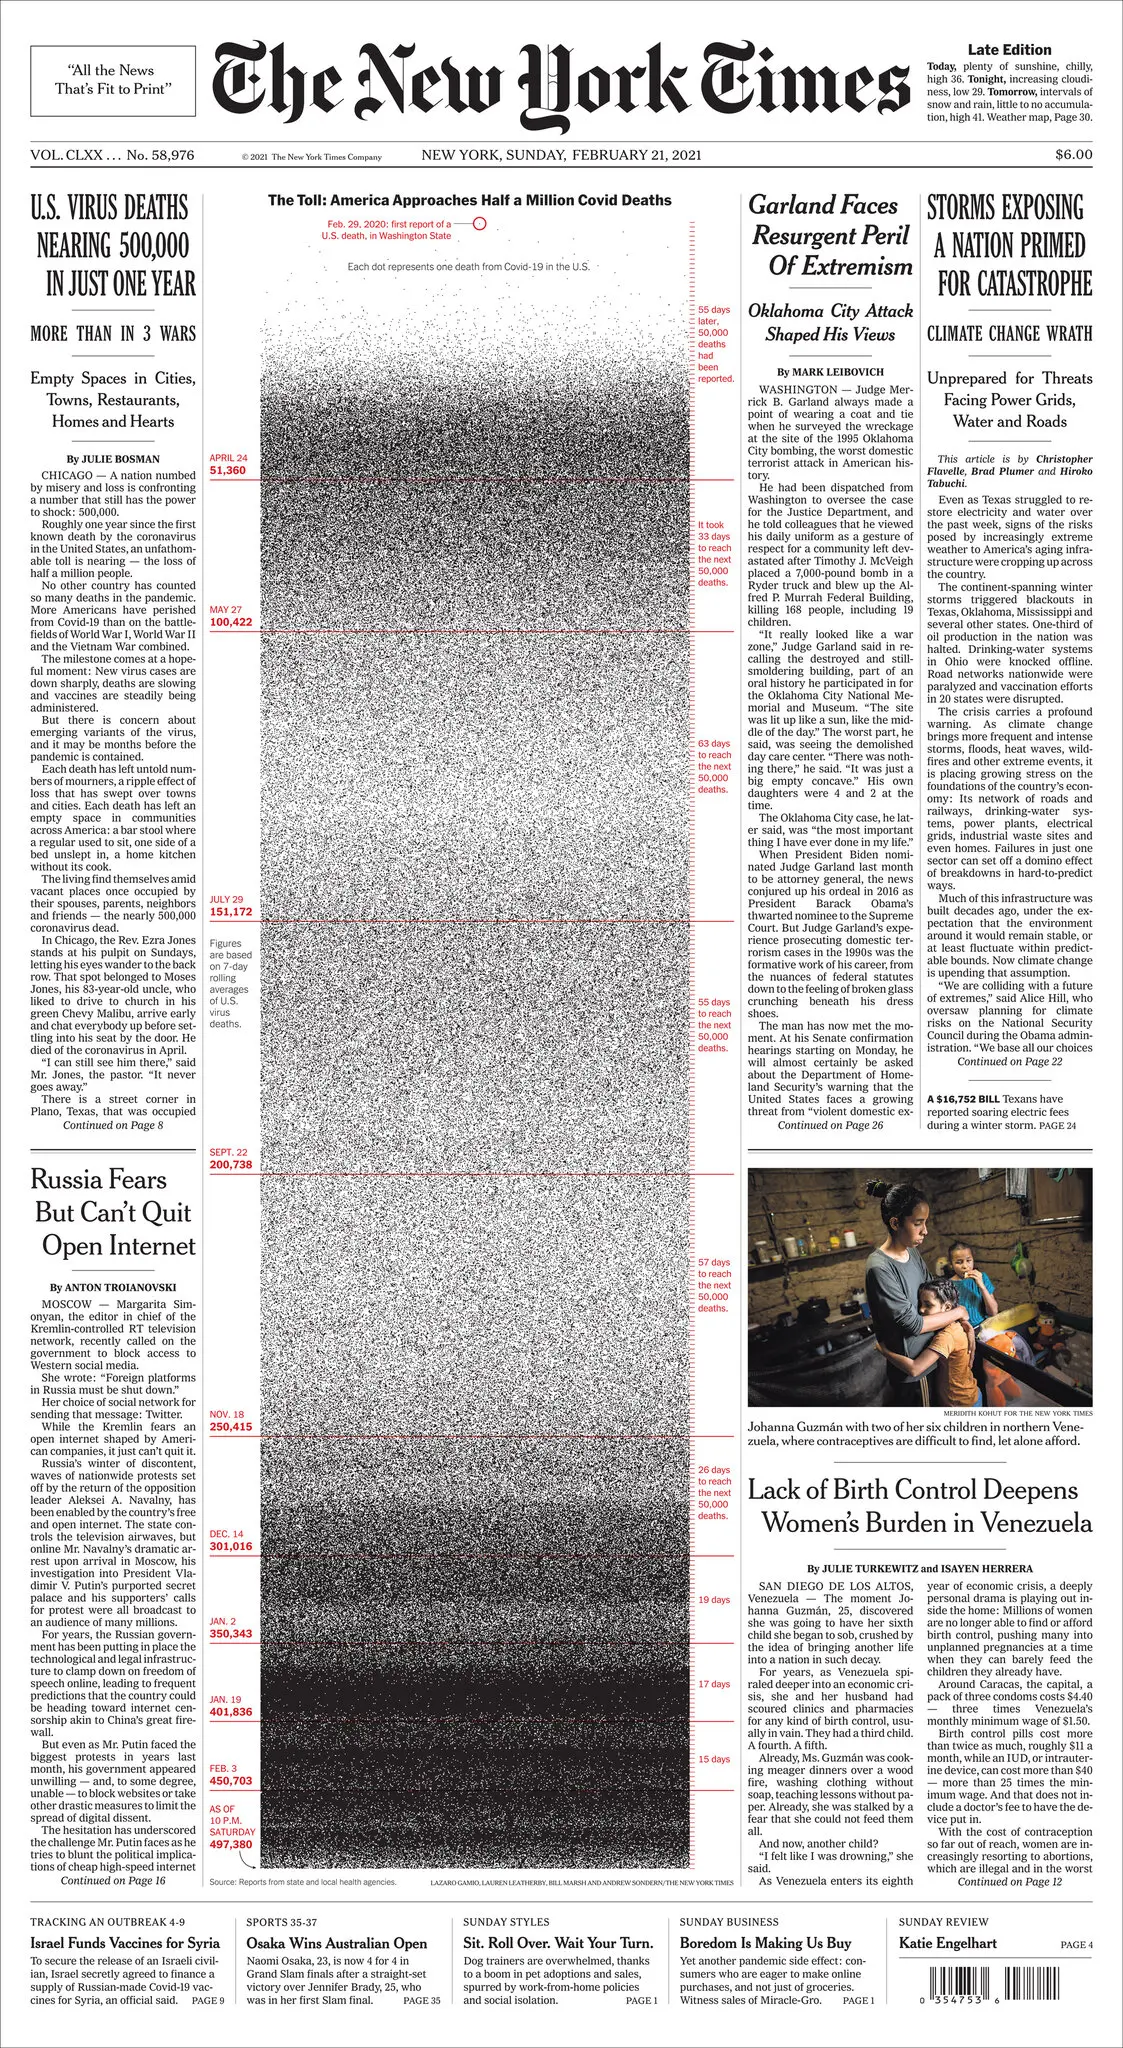
\includegraphics[height=.9\textheight]{nyt_500k.png}}
\only<3>{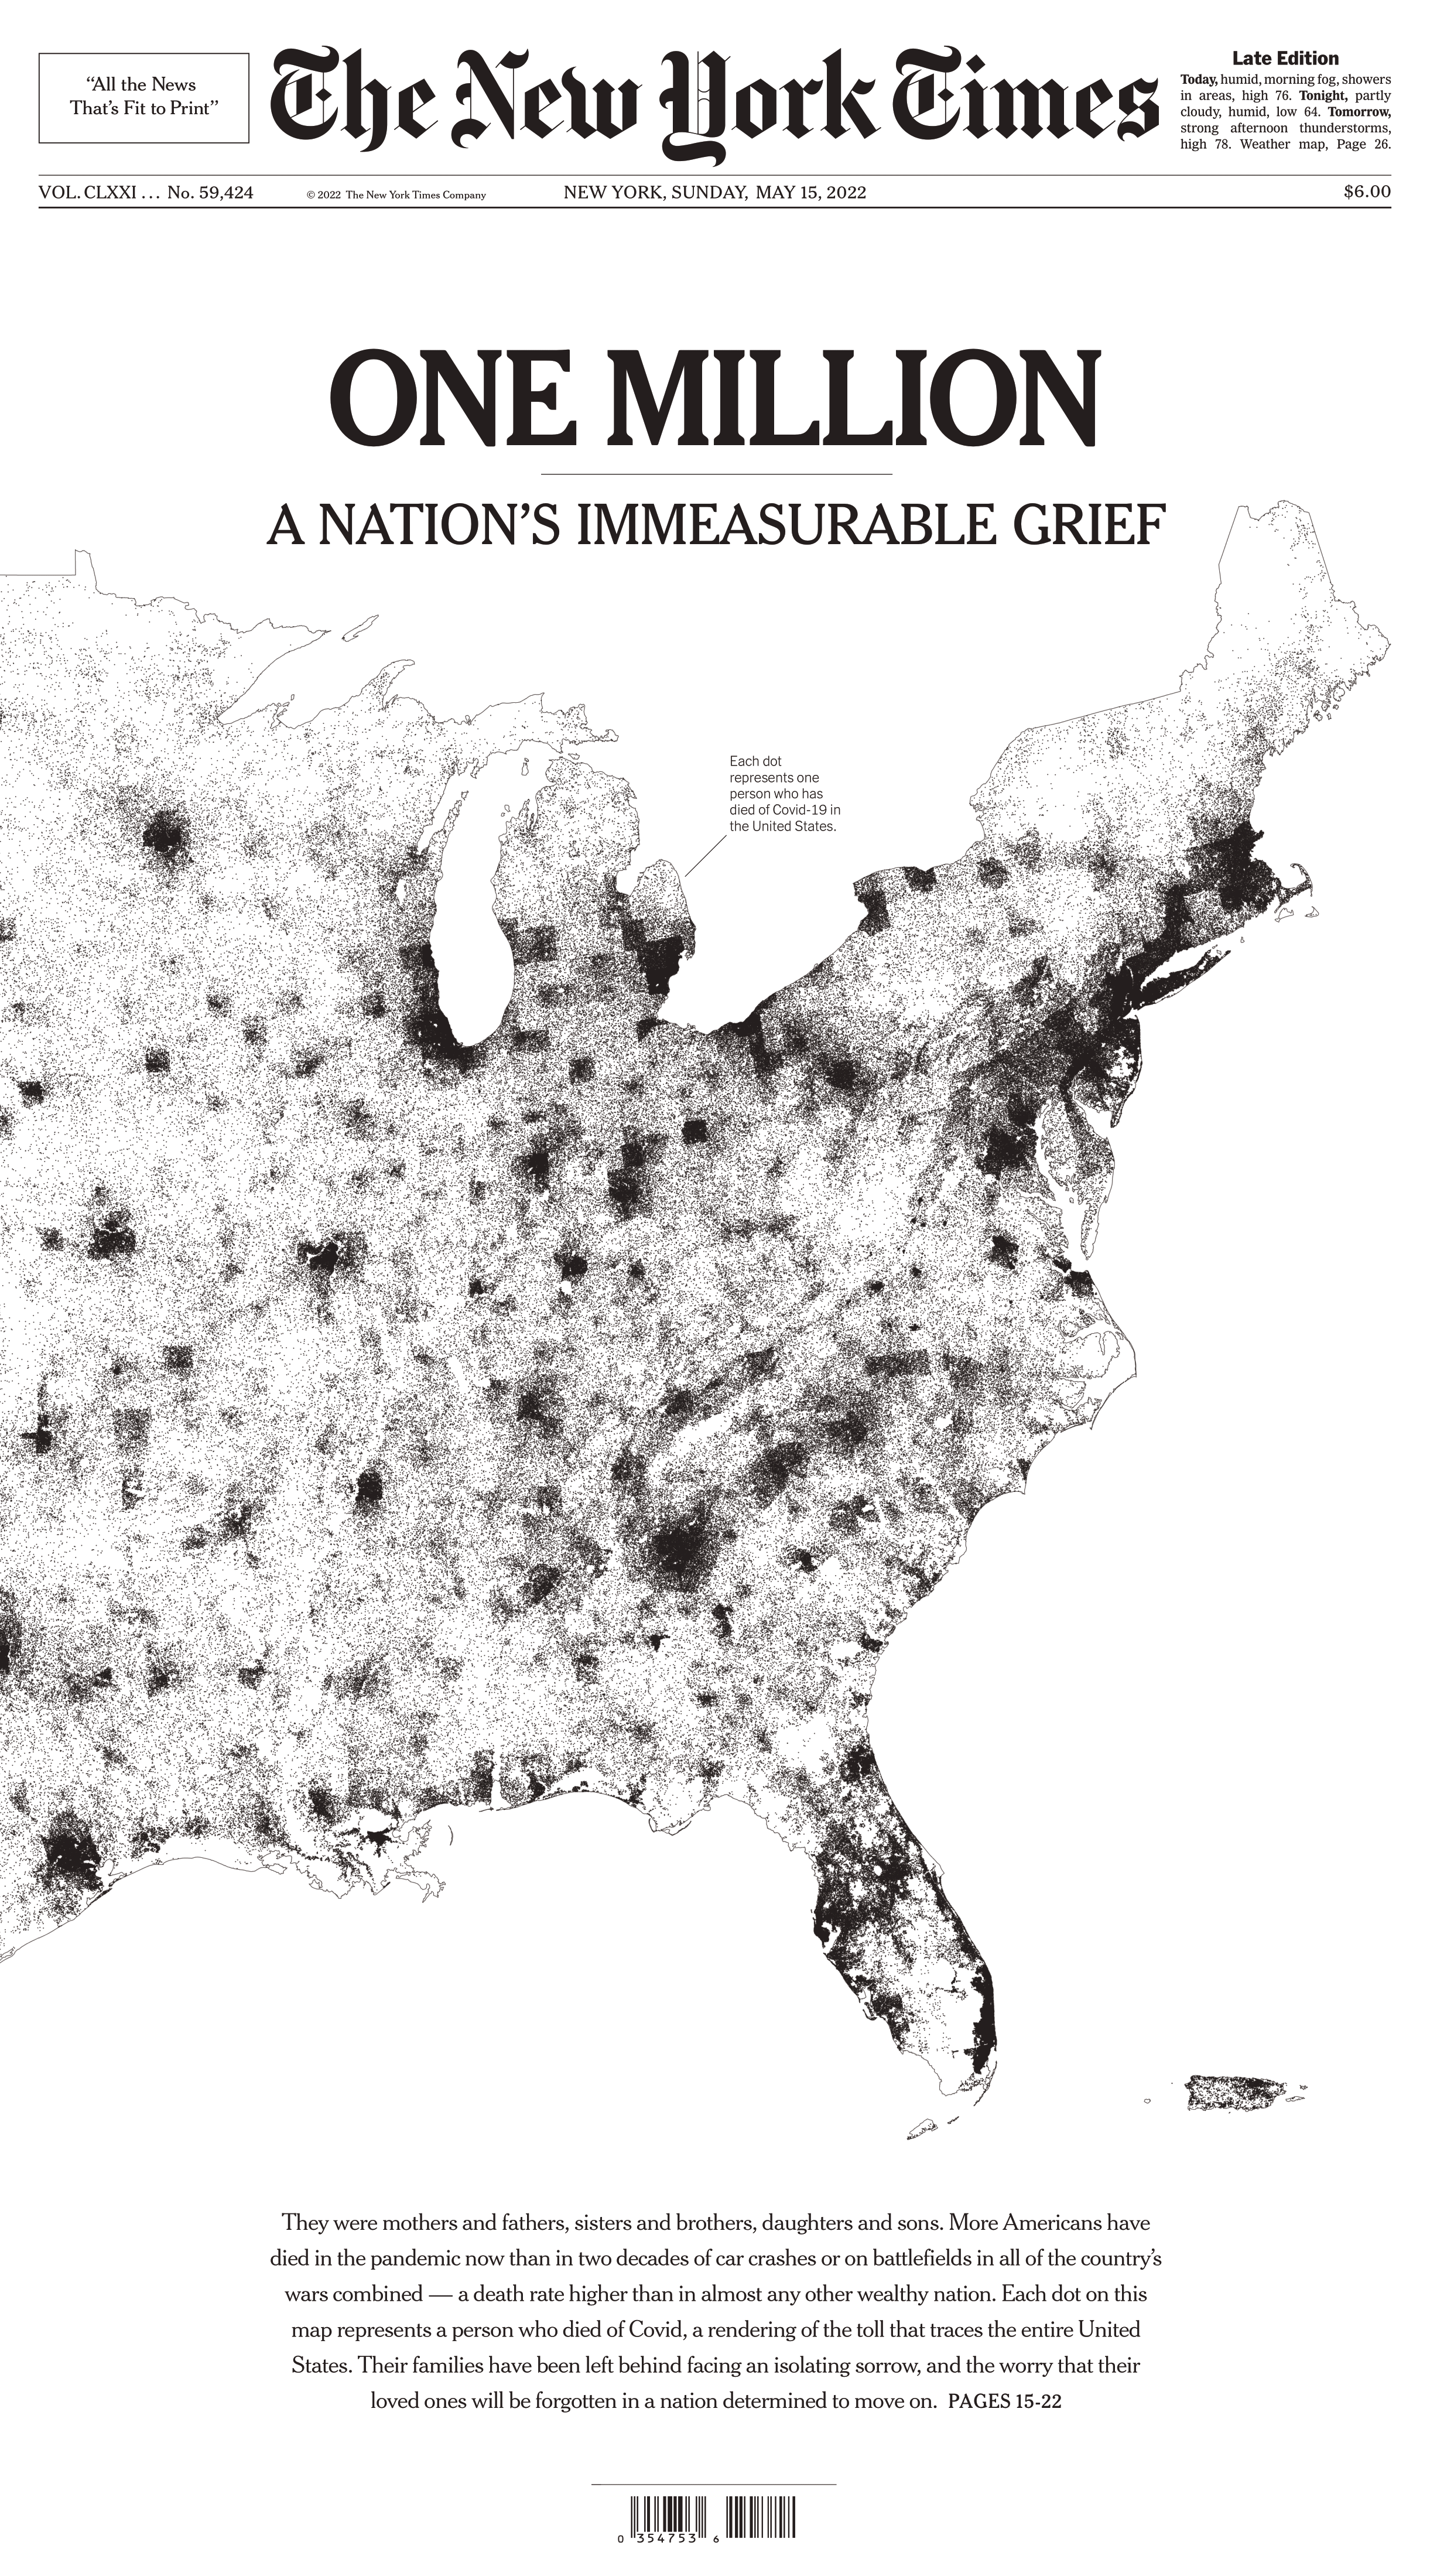
\includegraphics[height=.9\textheight]{nyt_one_million.png}}
\only<4>{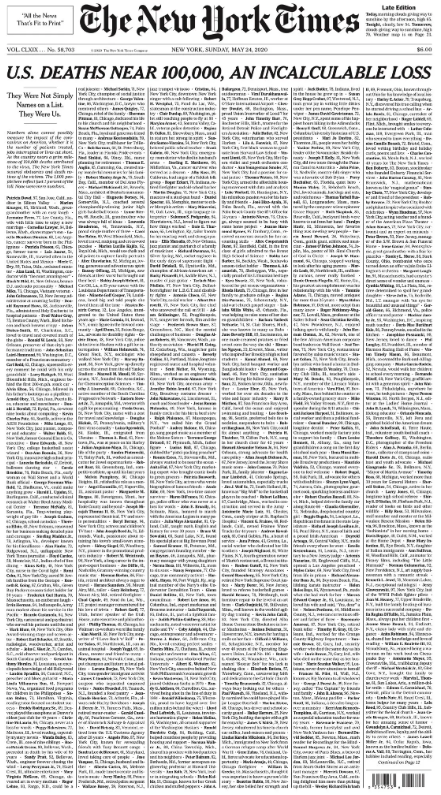
\includegraphics[height=.9\textheight]{nyt_incalculable_loss.png}}
\only<5>{
    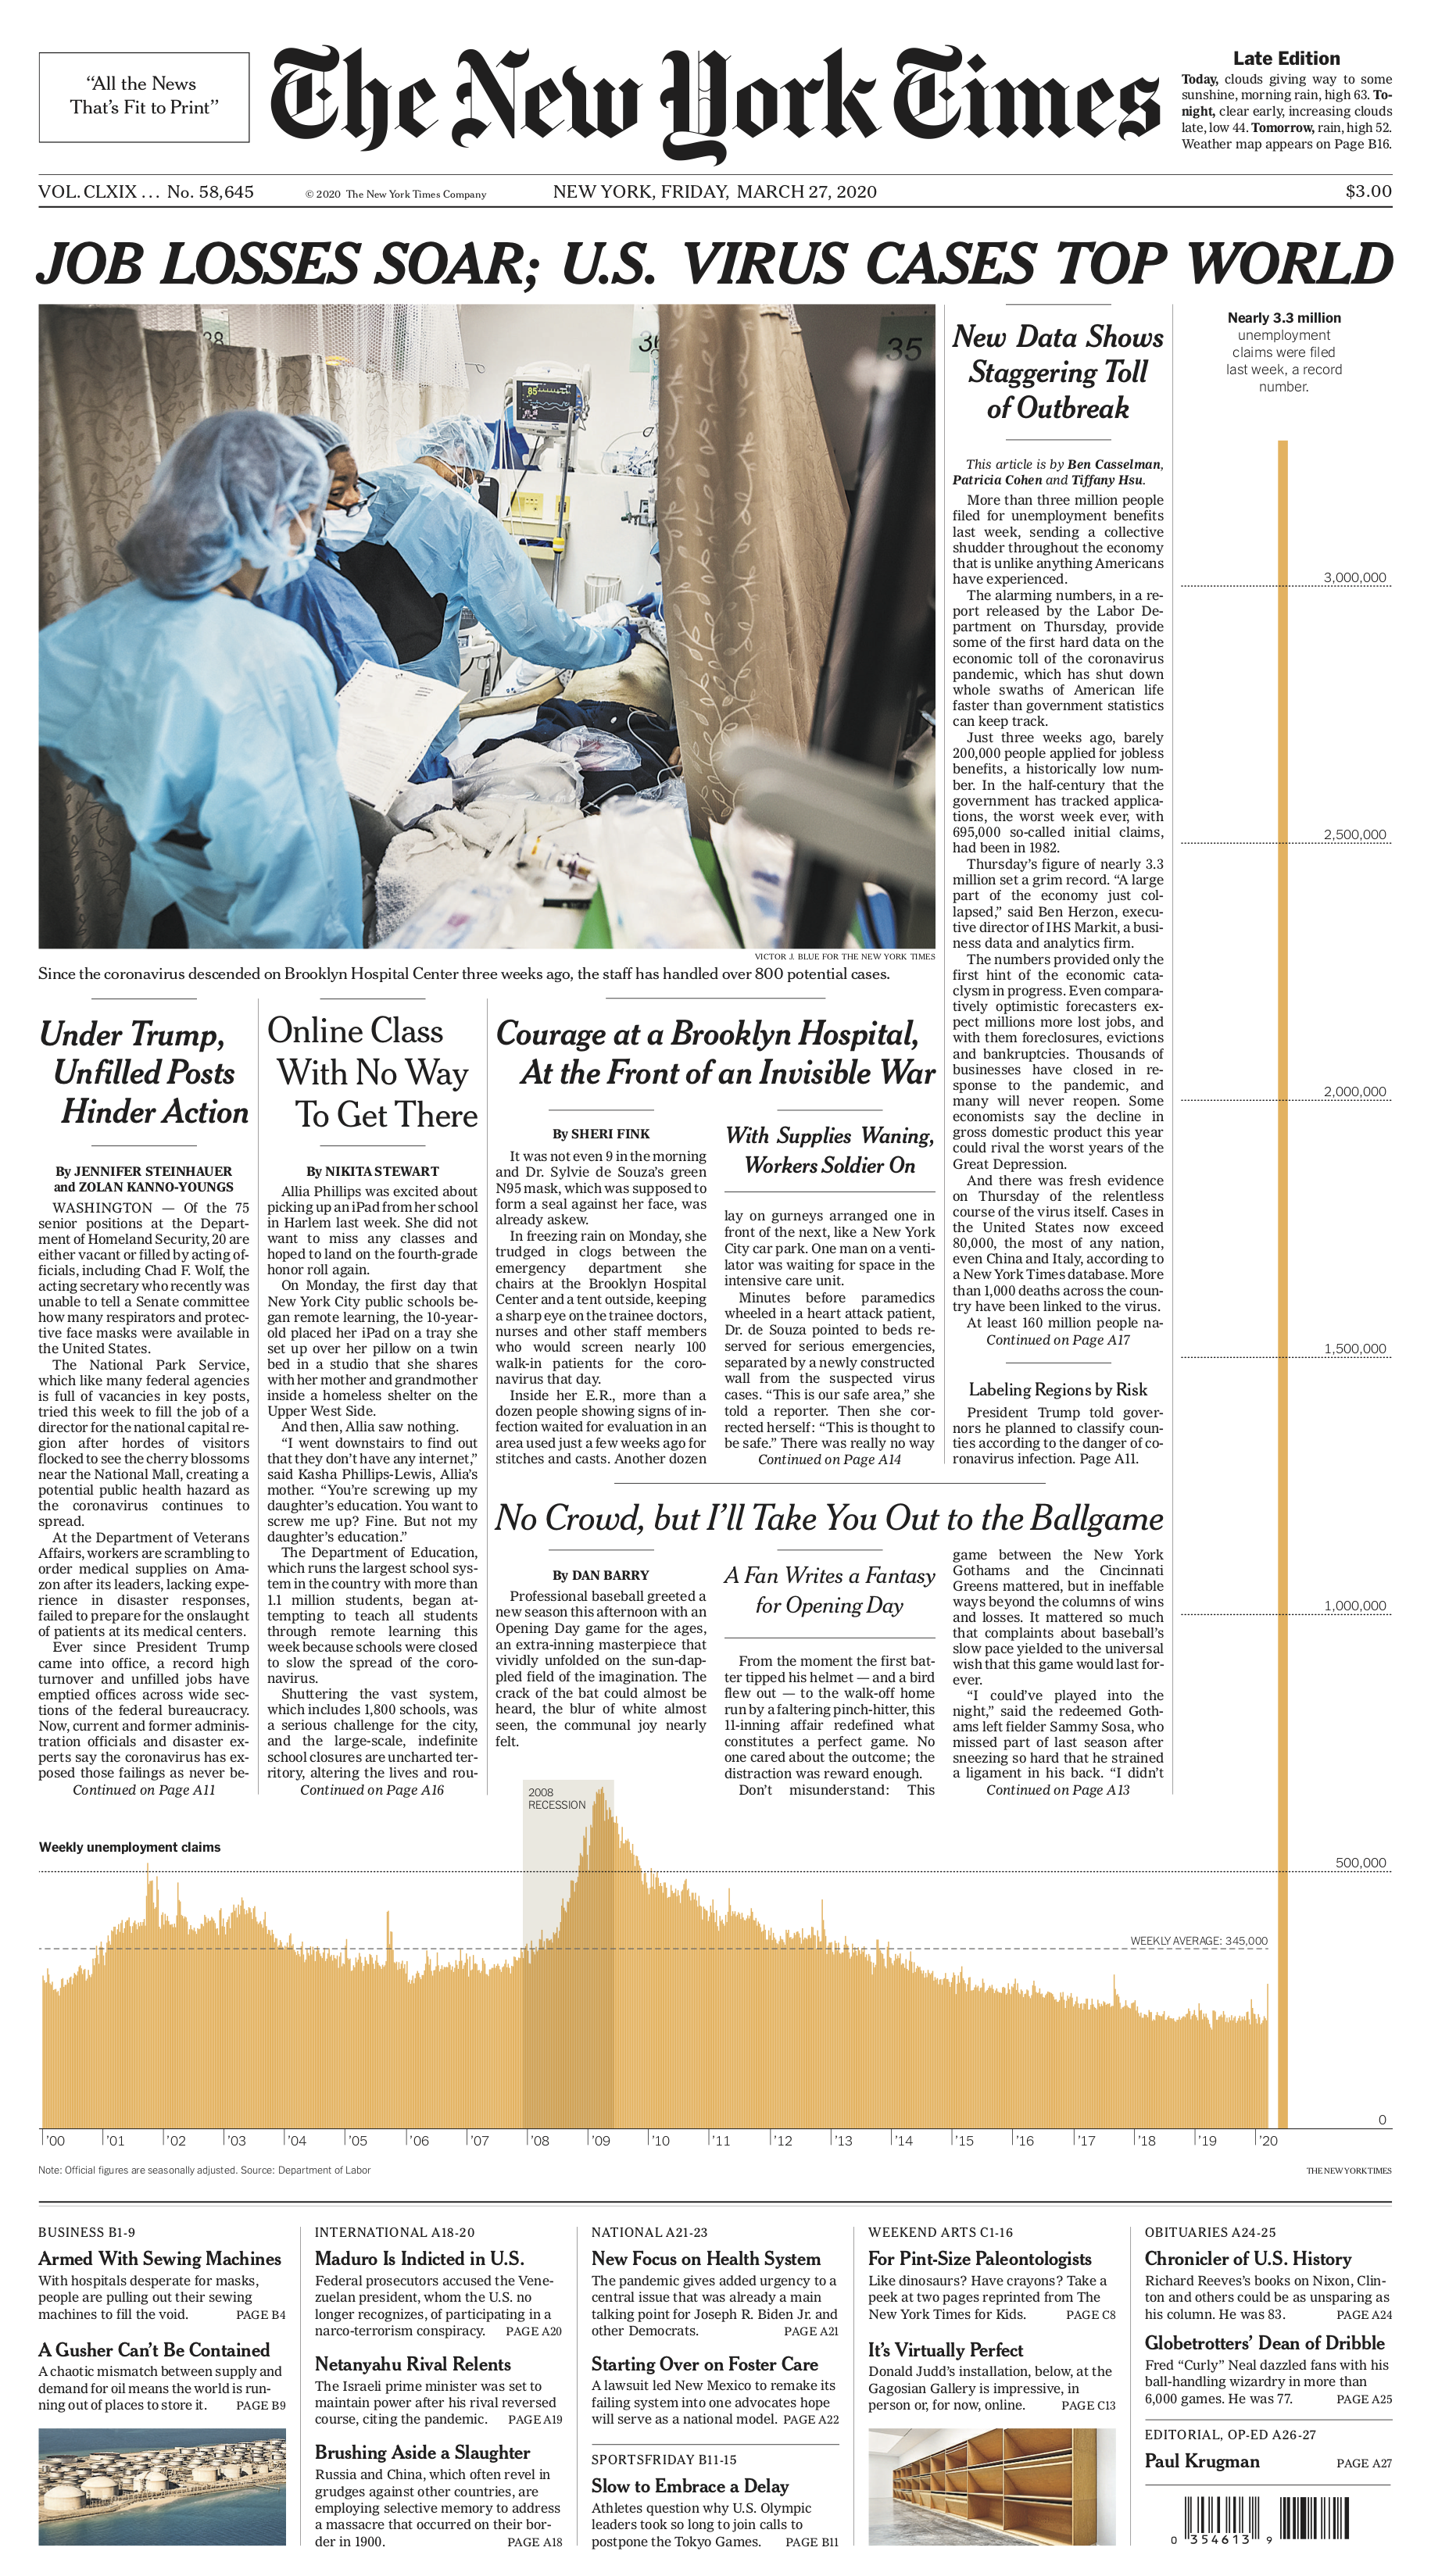
\includegraphics[width=.24\textwidth]{nyt_unemp.png} 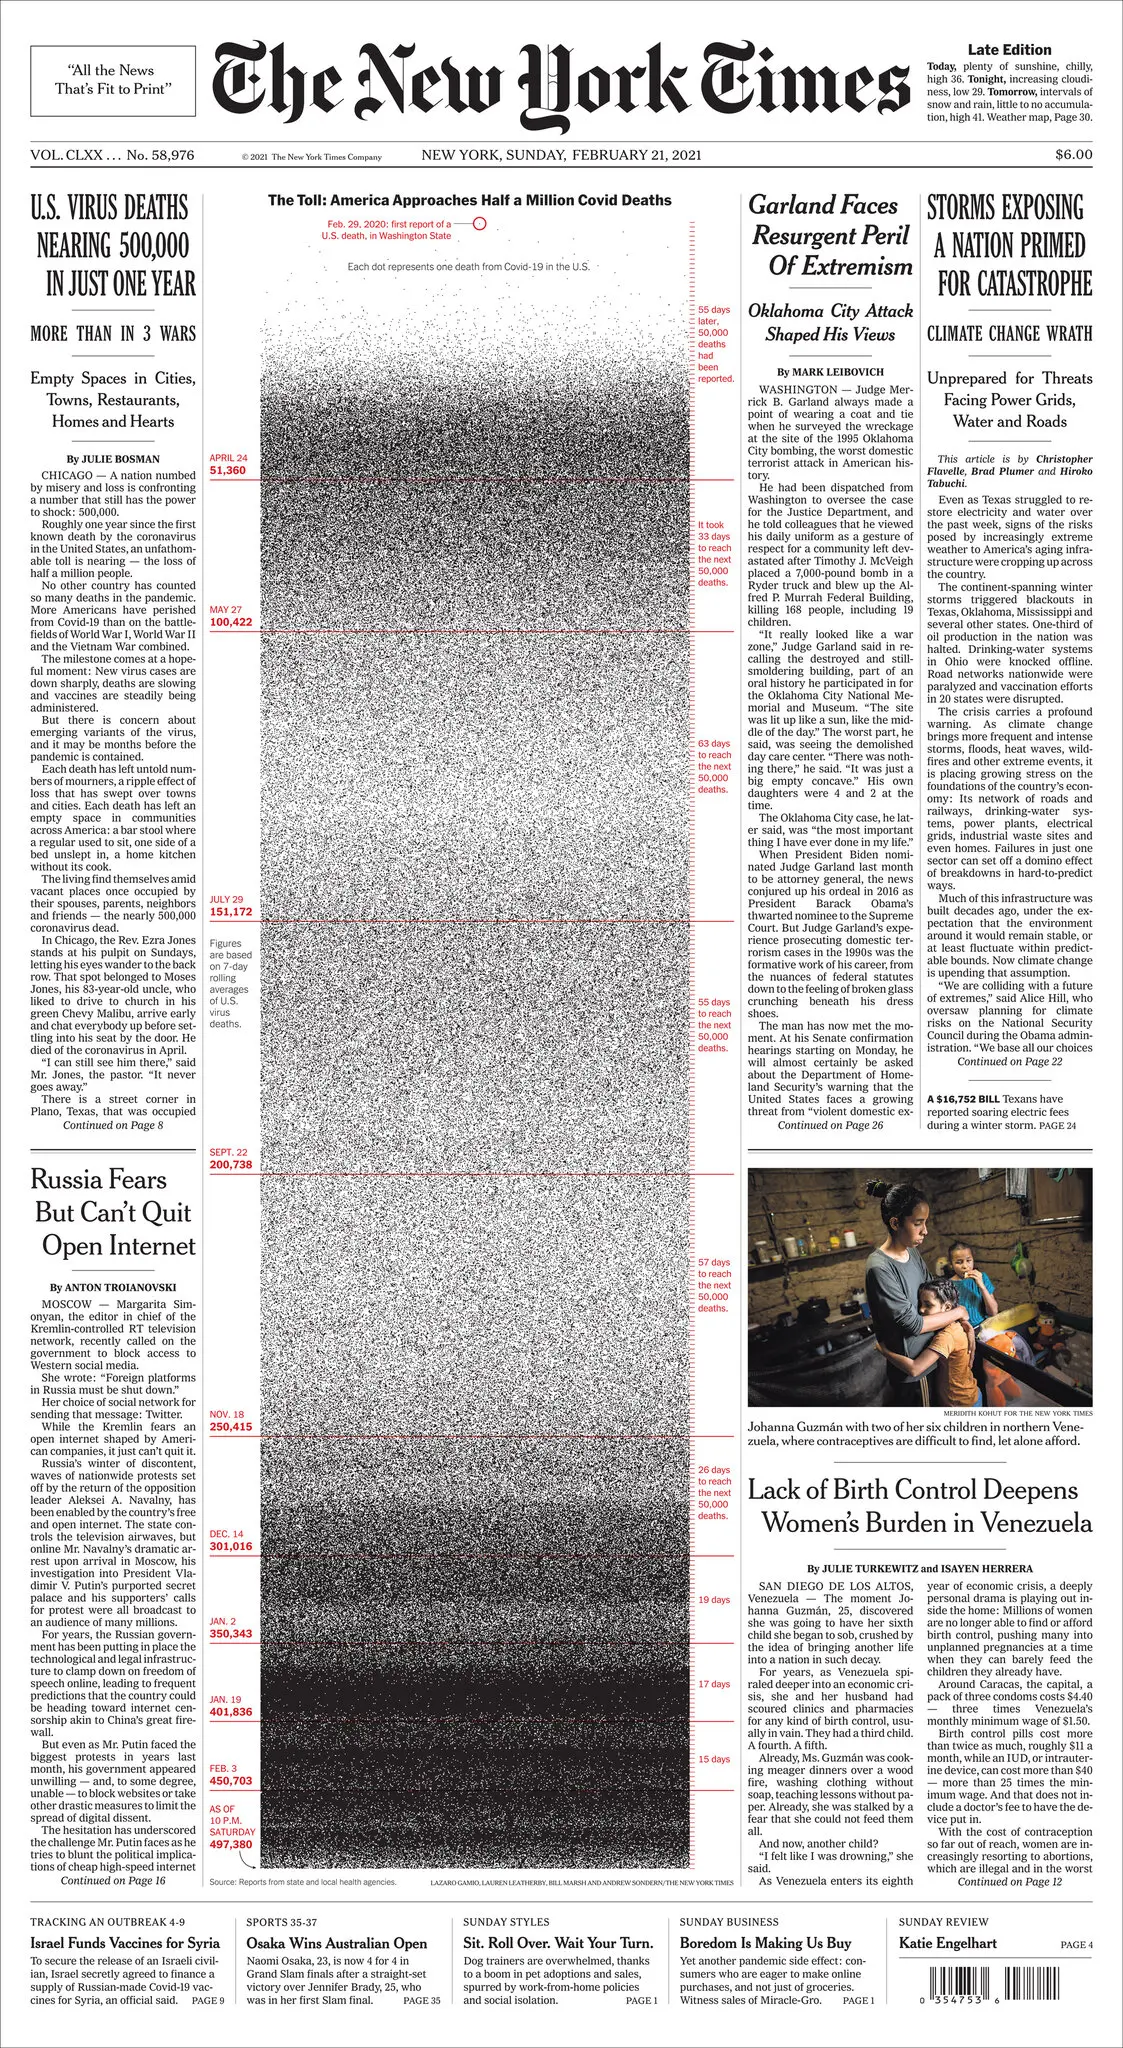
\includegraphics[width=.24\textwidth]{nyt_500k.png}
    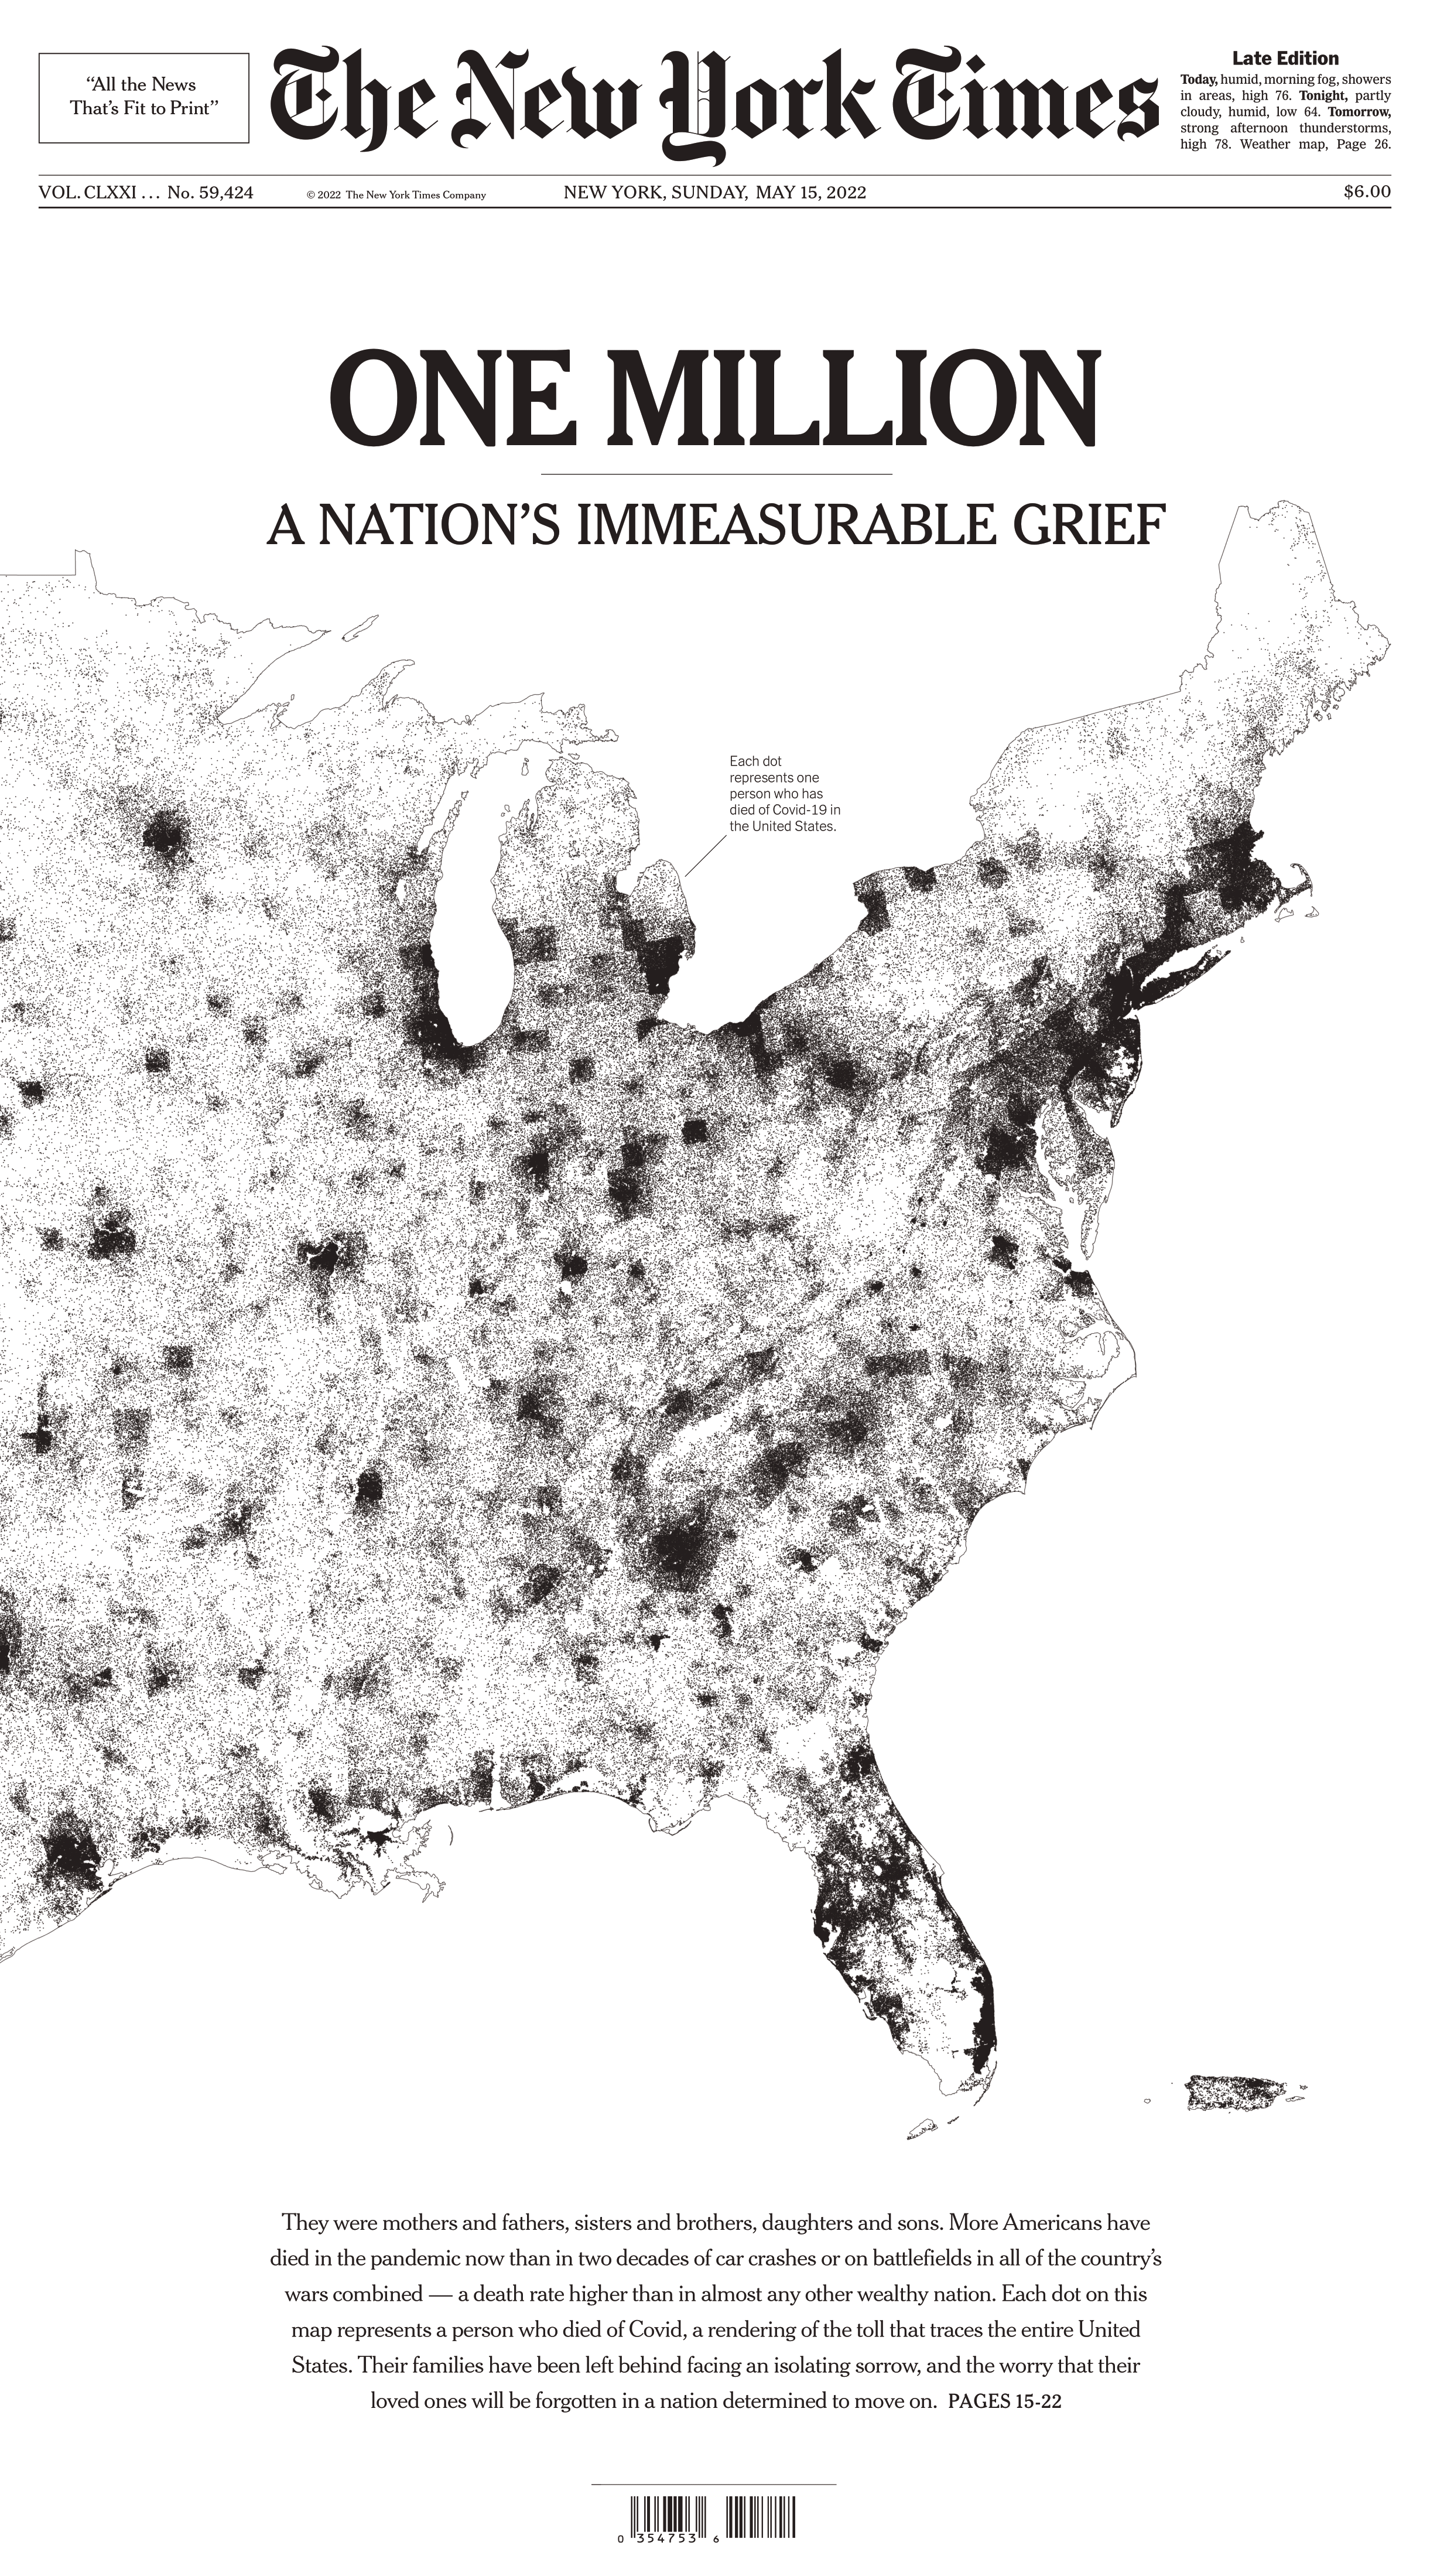
\includegraphics[width=.24\textwidth]{nyt_one_million.png} 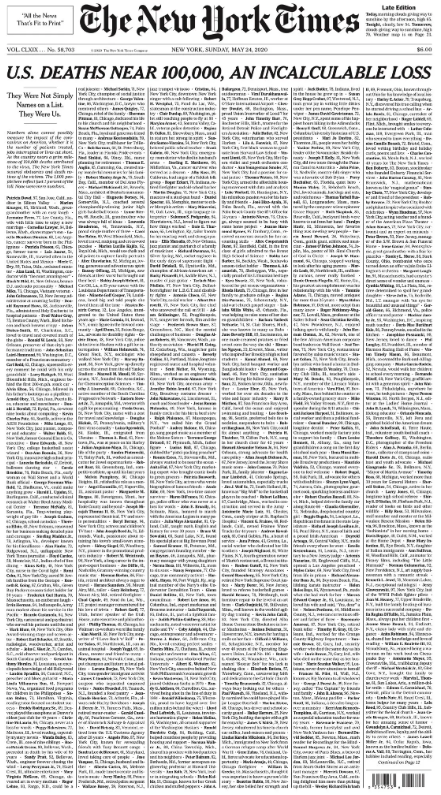
\includegraphics[width=.24\textwidth]{nyt_incalculable_loss.png}
}
}

%%%%%%%%%%%%%%%%%%%%%%%%%%%%%%%%%%%%%%%%%%%%%%%%%%%%%%%%%%%%%%%%%%
\frame{\frametitle{Early Data Visualization}
\only<1>{
    \centering
    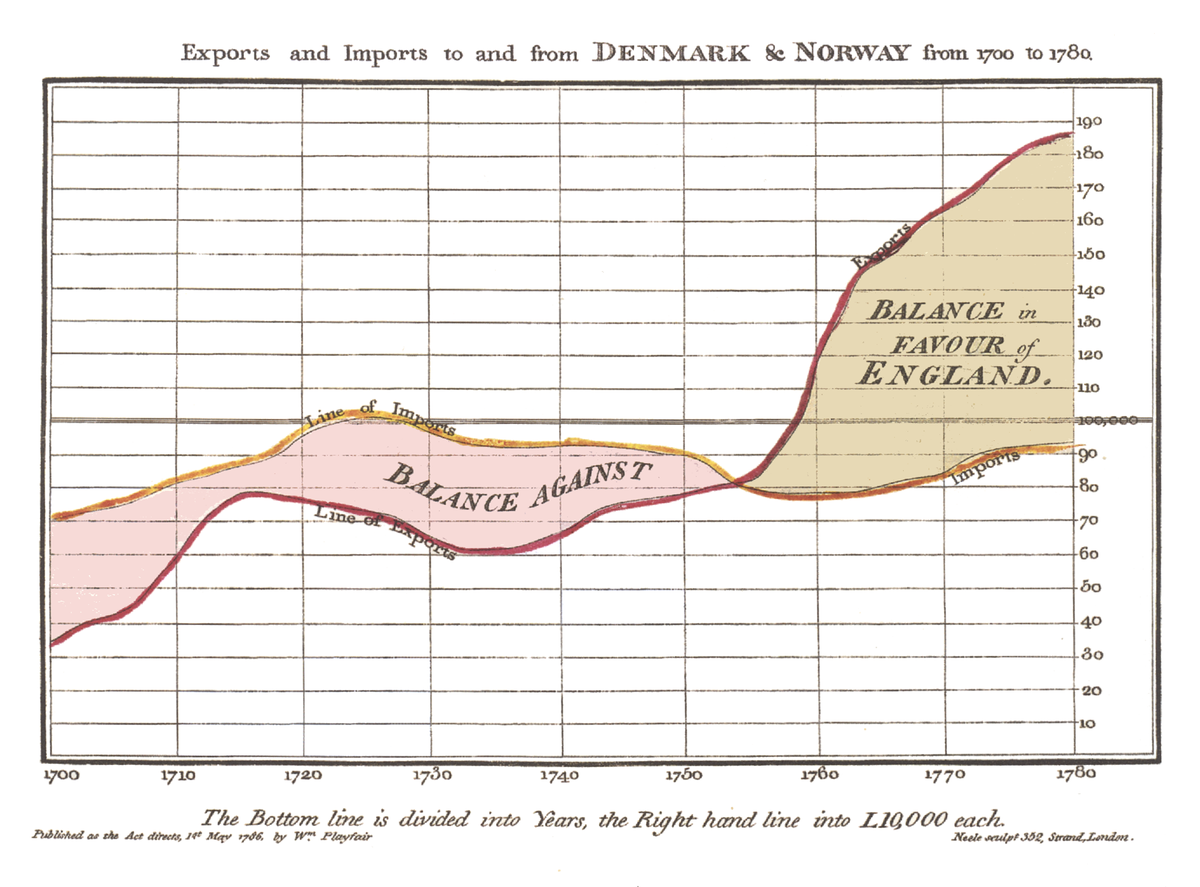
\includegraphics[height=.75\textheight]{Playfair.png}\\
    William Playfair (late 1700s)
}
\only<2>{
    \centering
    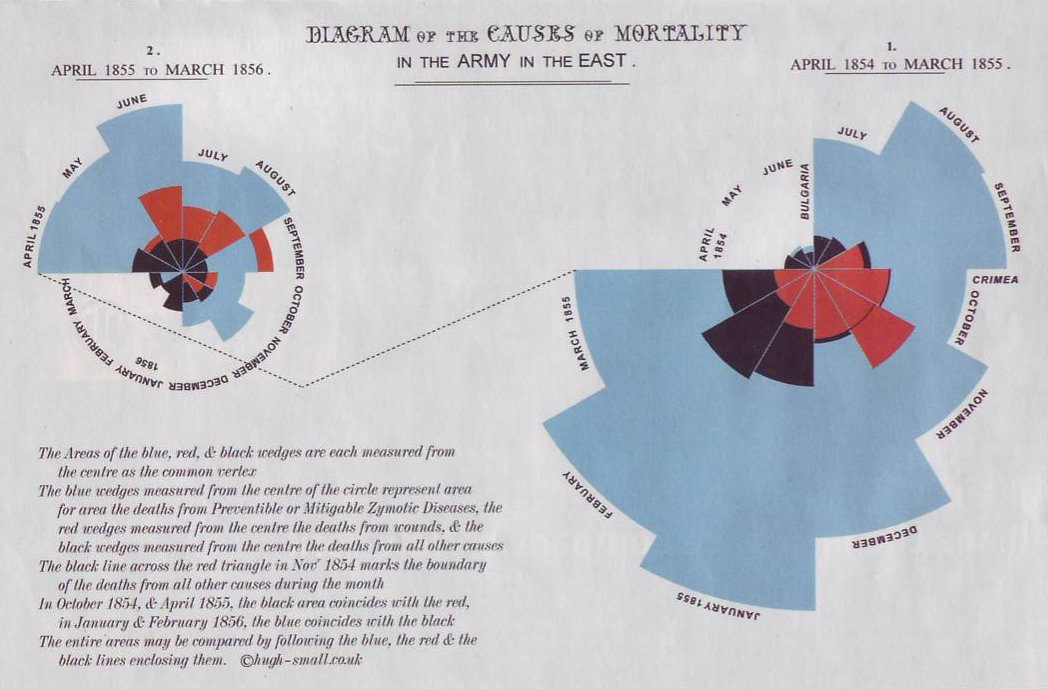
\includegraphics[height=.75\textheight]{Nightingale.jpg}\\
    Florence Nightingale (1858)
}
\only<3>{
    \centering
    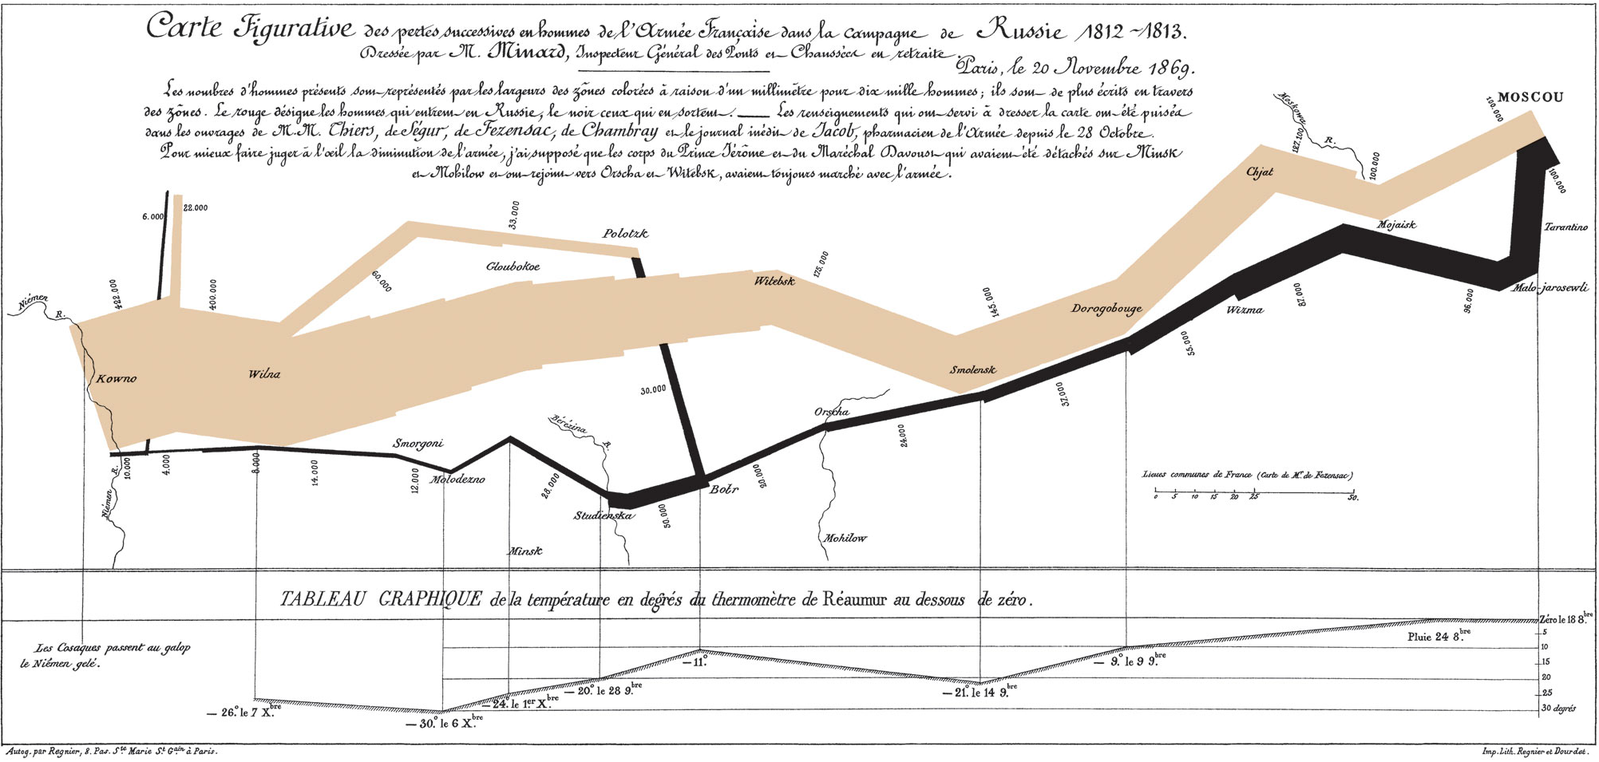
\includegraphics[width=\textwidth]{Minard.png}\\
    Charles Minard (1861)
}
}

%%%%%%%%%%%%%%%%%%%%%%%%%%%%%%%%%%%%%%%%%%%%%%%%%%%%%%%%%%%%%%%%%%

\frame{\frametitle{Edward Tufte}
\only<1-3, 8>{
    Published \textit{The Visual Display of Quantitative Information} in 1983\\
    ~\\
    \begin{enumerate}[<+(1)->]
        \item ``Above all else, show the data.''
        \item Maximize the amount of data and minimize the amount of ink
        \item<8> Opponent of unnecessary graphical design (``chartjunk'')
    \end{enumerate}
}

\only<4>{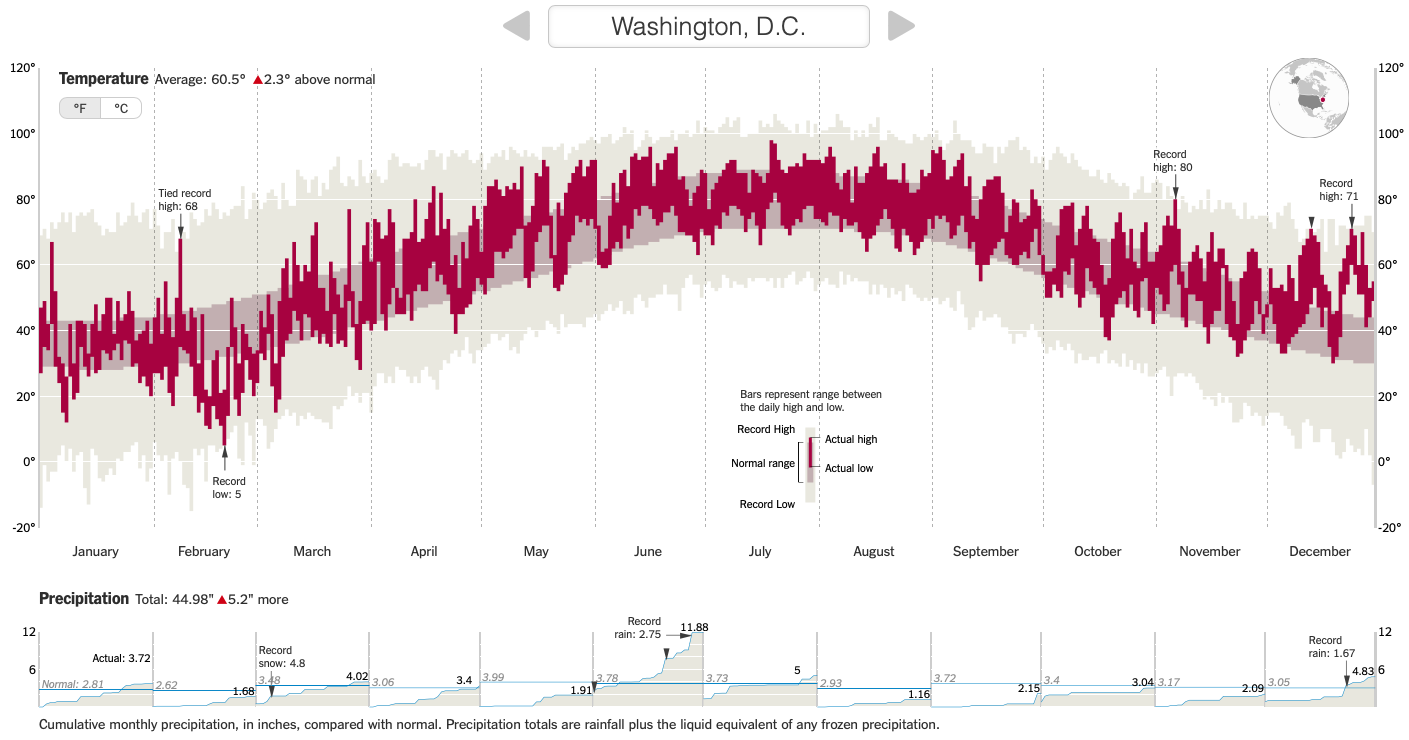
\includegraphics[width=\textwidth]{nyt_modern.png}}
\only<5>{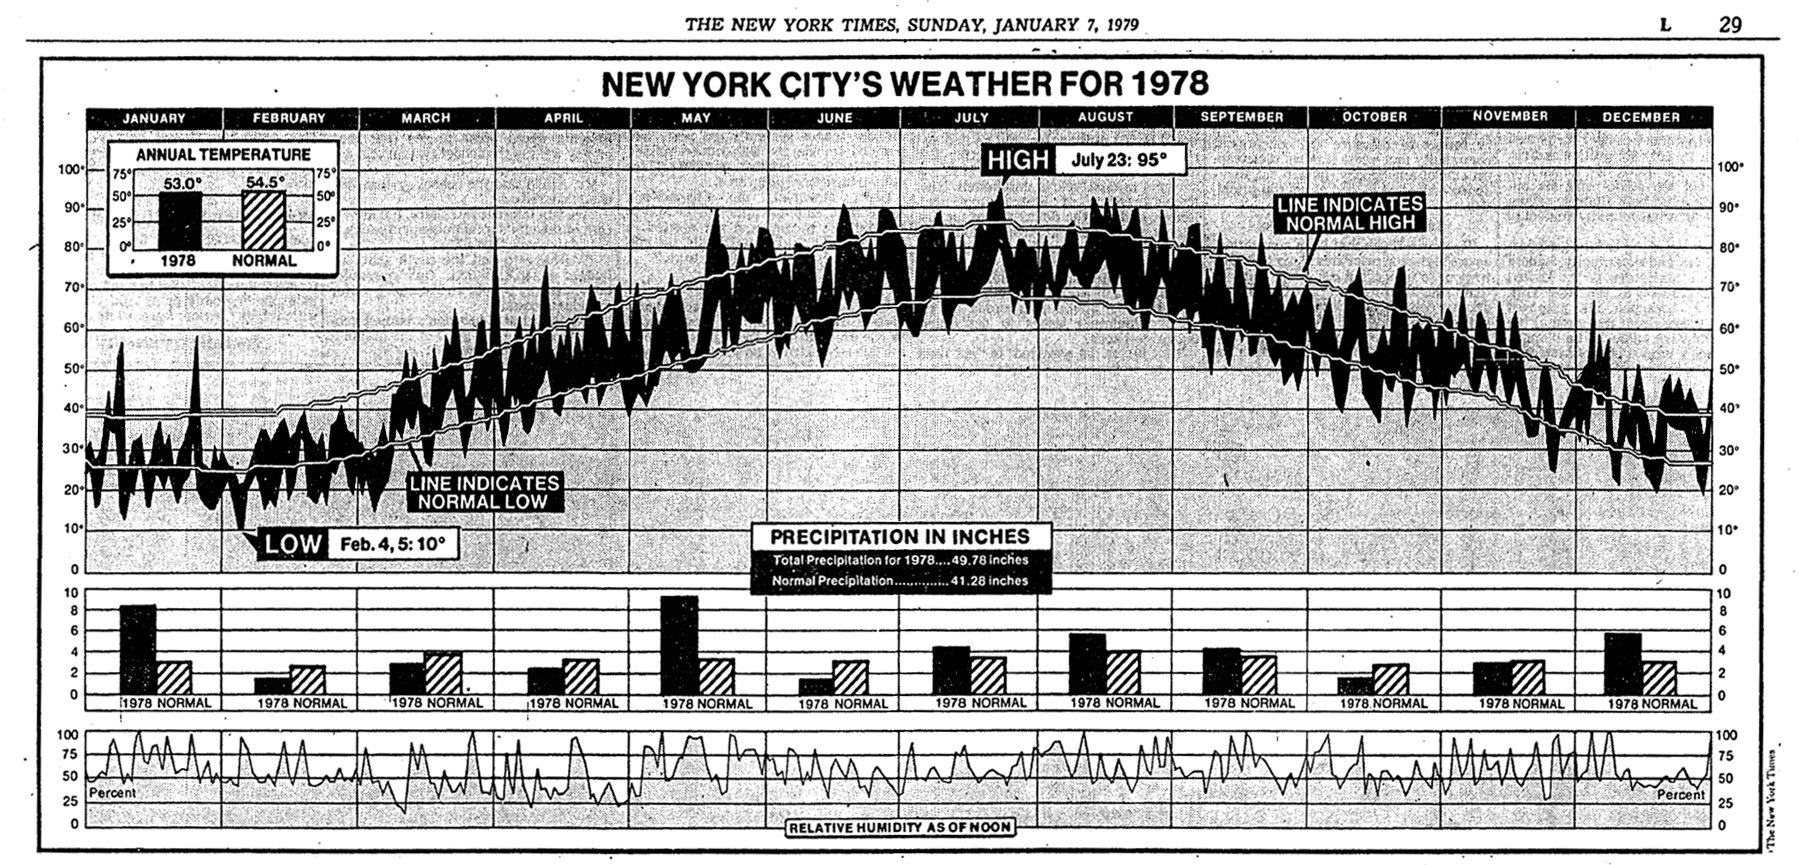
\includegraphics[width=\textwidth]{nyt_weather_1979.jpg}}
\only<6>{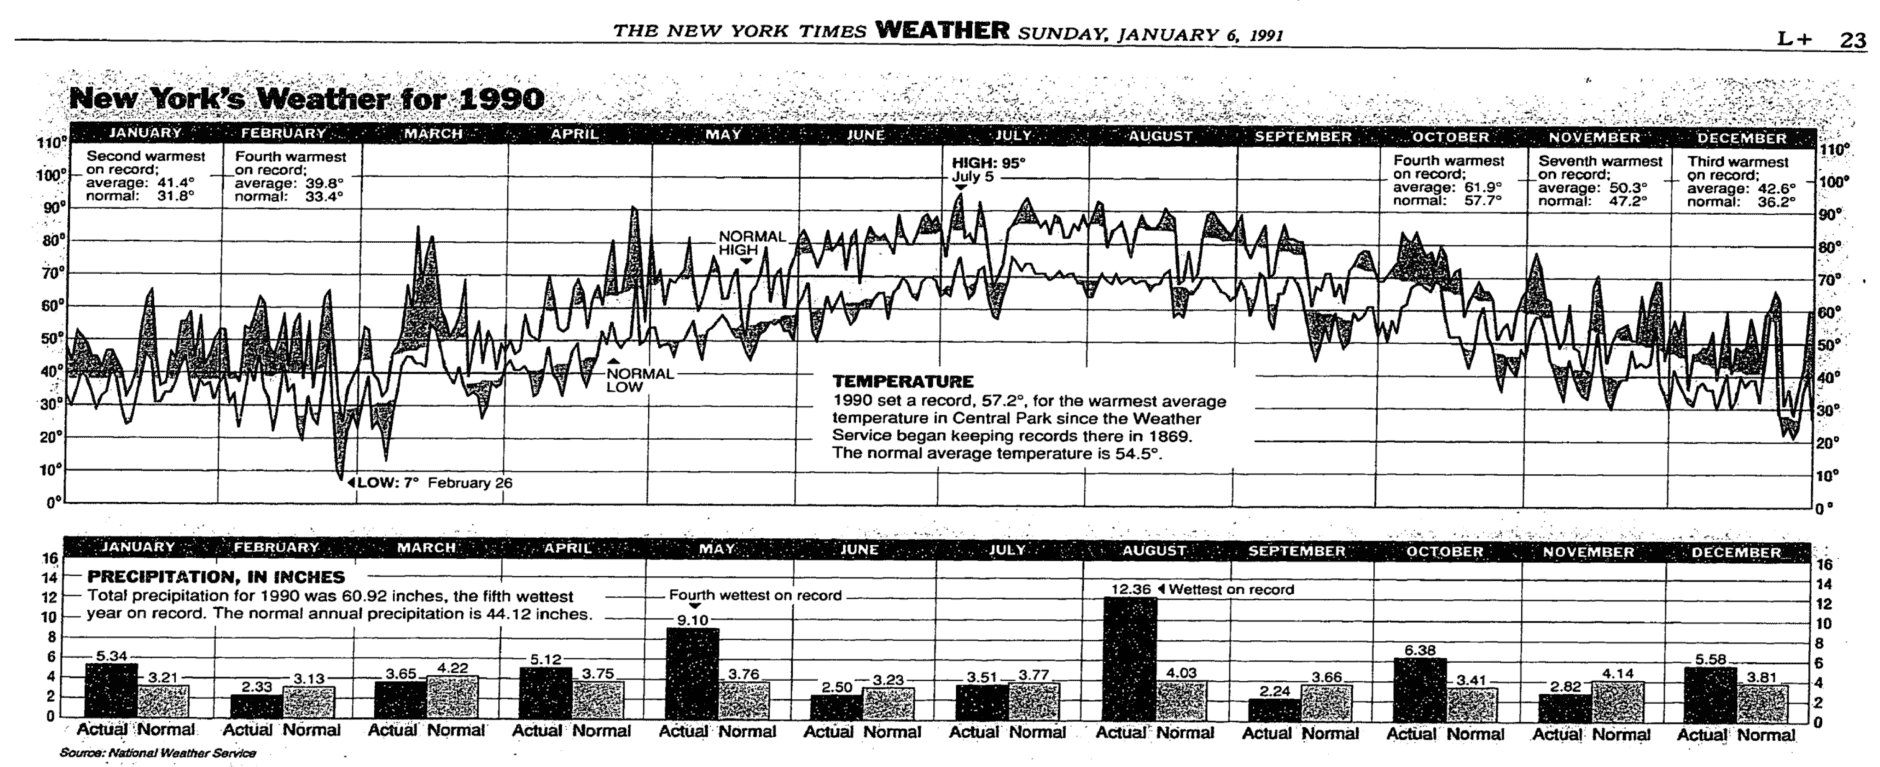
\includegraphics[width=\textwidth]{nyt_weather_1991.png}}
\only<7>{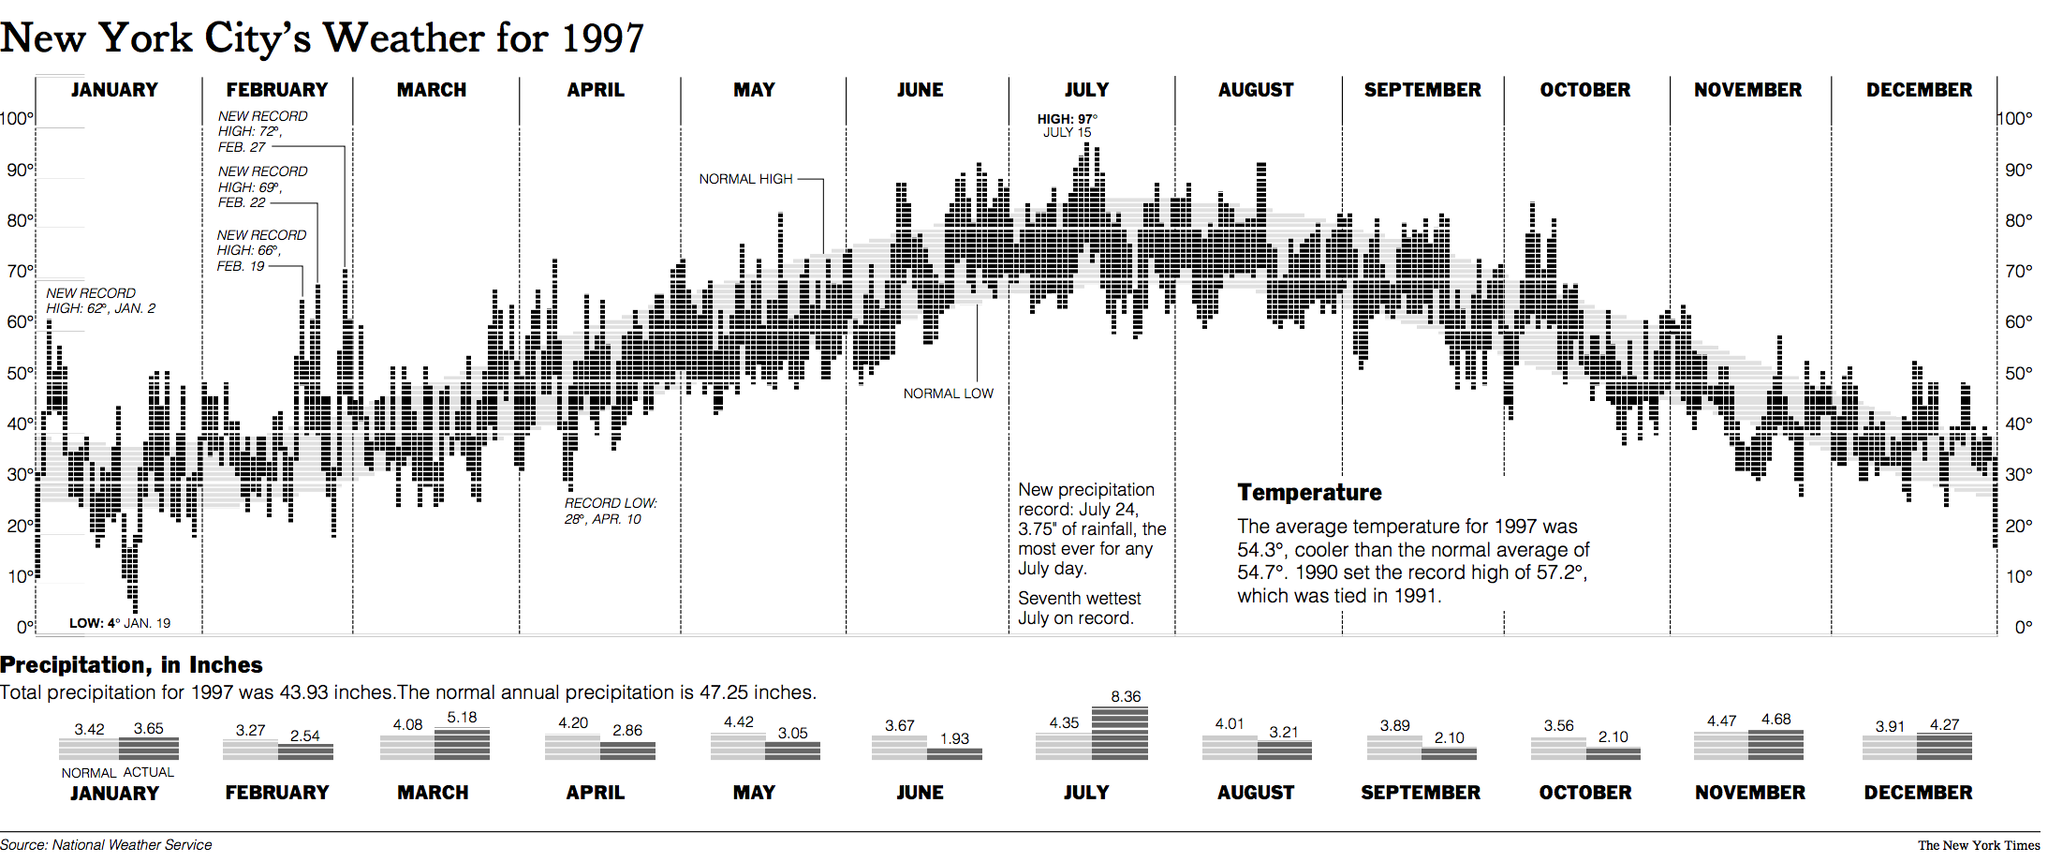
\includegraphics[width=\textwidth]{nyt_weather_1998.png}}
\only<9>{\centering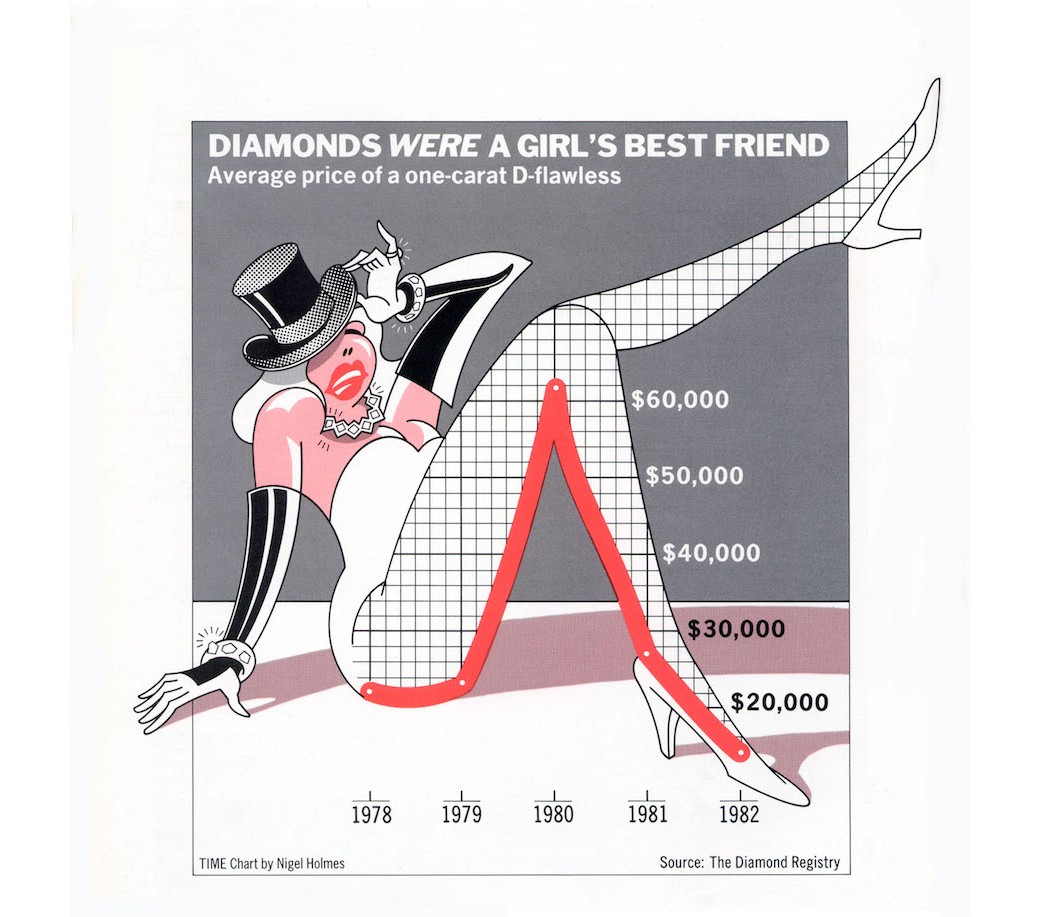
\includegraphics[height=.8\textheight]{holmes.jpg}}
\only<10>{\centering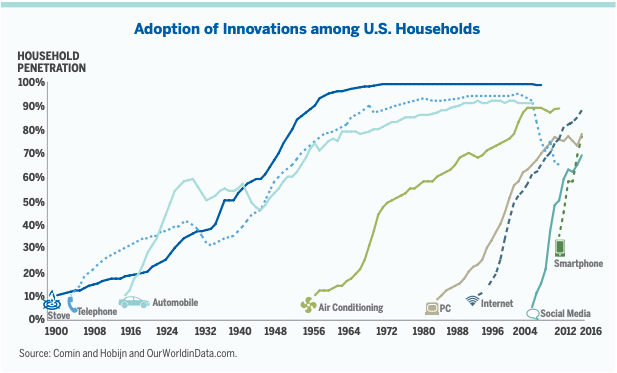
\includegraphics[width=.9\textwidth]{tech_adoption.png}\\\scriptsize Source: Fred Alger \& Co., Inc.}
}

%%%%%%%%%%%%%%%%%%%%%%%%%%%%%%%%%%%%%%%%%%%%%%%%%%%%%%%%%%%%%%%%%%
\frame{\frametitle{Engineers vs. Designers}
\only<1>{
    \begin{center}
    \begin{tabularx}{.9\textwidth}{|*{2}{X|}}
    \hline
    \textbf{Engineers} & \textbf{Designers} \\
    \hline
    $\bullet$ Simplicity of design & $\bullet$ Artistic expression \\
    $\bullet$ Maximize the data & $\bullet$ Express only a few ideas \\
    $\bullet$ Assumes the viewer is alert and interested & $\bullet$ Assumes the viewer is inattentive \\
    $\bullet$ Form follows function & $\bullet$ Many forms can convey the same data \\
    \hline
    \end{tabularx}
    \end{center}
}

\only<2>{\centering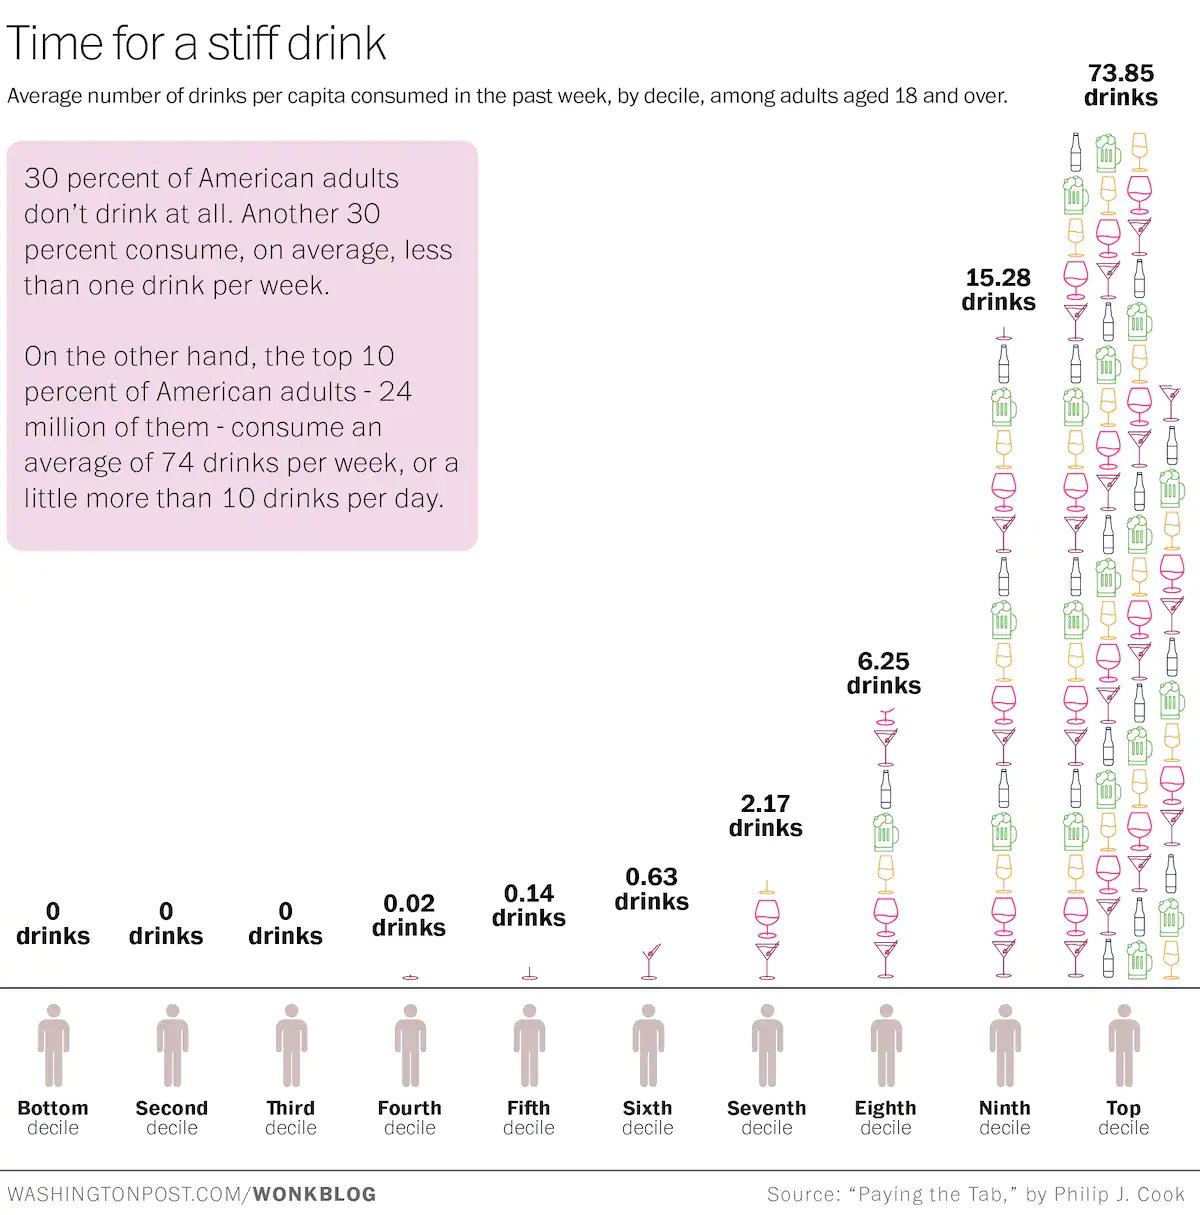
\includegraphics[height=.8\textheight]{us_drinking.jpg}}
}

%%%%%%%%%%%%%%%%%%%%%%%%%%%%%%%%%%%%%%%%%%%%%%%%%%%%%%%%%%%%%%%%%%
\frame{\frametitle{Science of Data Visualization}
\only<1>{
    \huge
    \begin{center}
    Sight \MVRightarrow{} Perception \MVRightarrow{} Cognition
    \end{center}
}

\only<2-4>{
    {\Large \textbf{Sight}}
    \begin{itemize}[<+(1)->]
        \item The eyes send small snapshots of high-resolution focus to the brain, which puts the snapshots together into a single image
        \item The order in which the eyes take these snapshots is not random -- it is optimized through evolution (i.e., moving objects, pure colors get attention first)
        \item When we design data visualization, the first question to ask is: \textbf{where do my eyes go first?}
    \end{itemize}
}

\only<5-6,17>{
    {\Large \textbf{Perception}}
    \begin{itemize}[<+(4)->]
        \item Known as ``preattentive features''
        \item The brain is optimized to quickly identify contrasts in color and recognize groups
        \item<17> After ``where do my eyes go first?'', the next question is: \textbf{what is the first idea that comes to mind?}
    \end{itemize}
}

\only<7>{\centering\large Color Contrasts\\~\\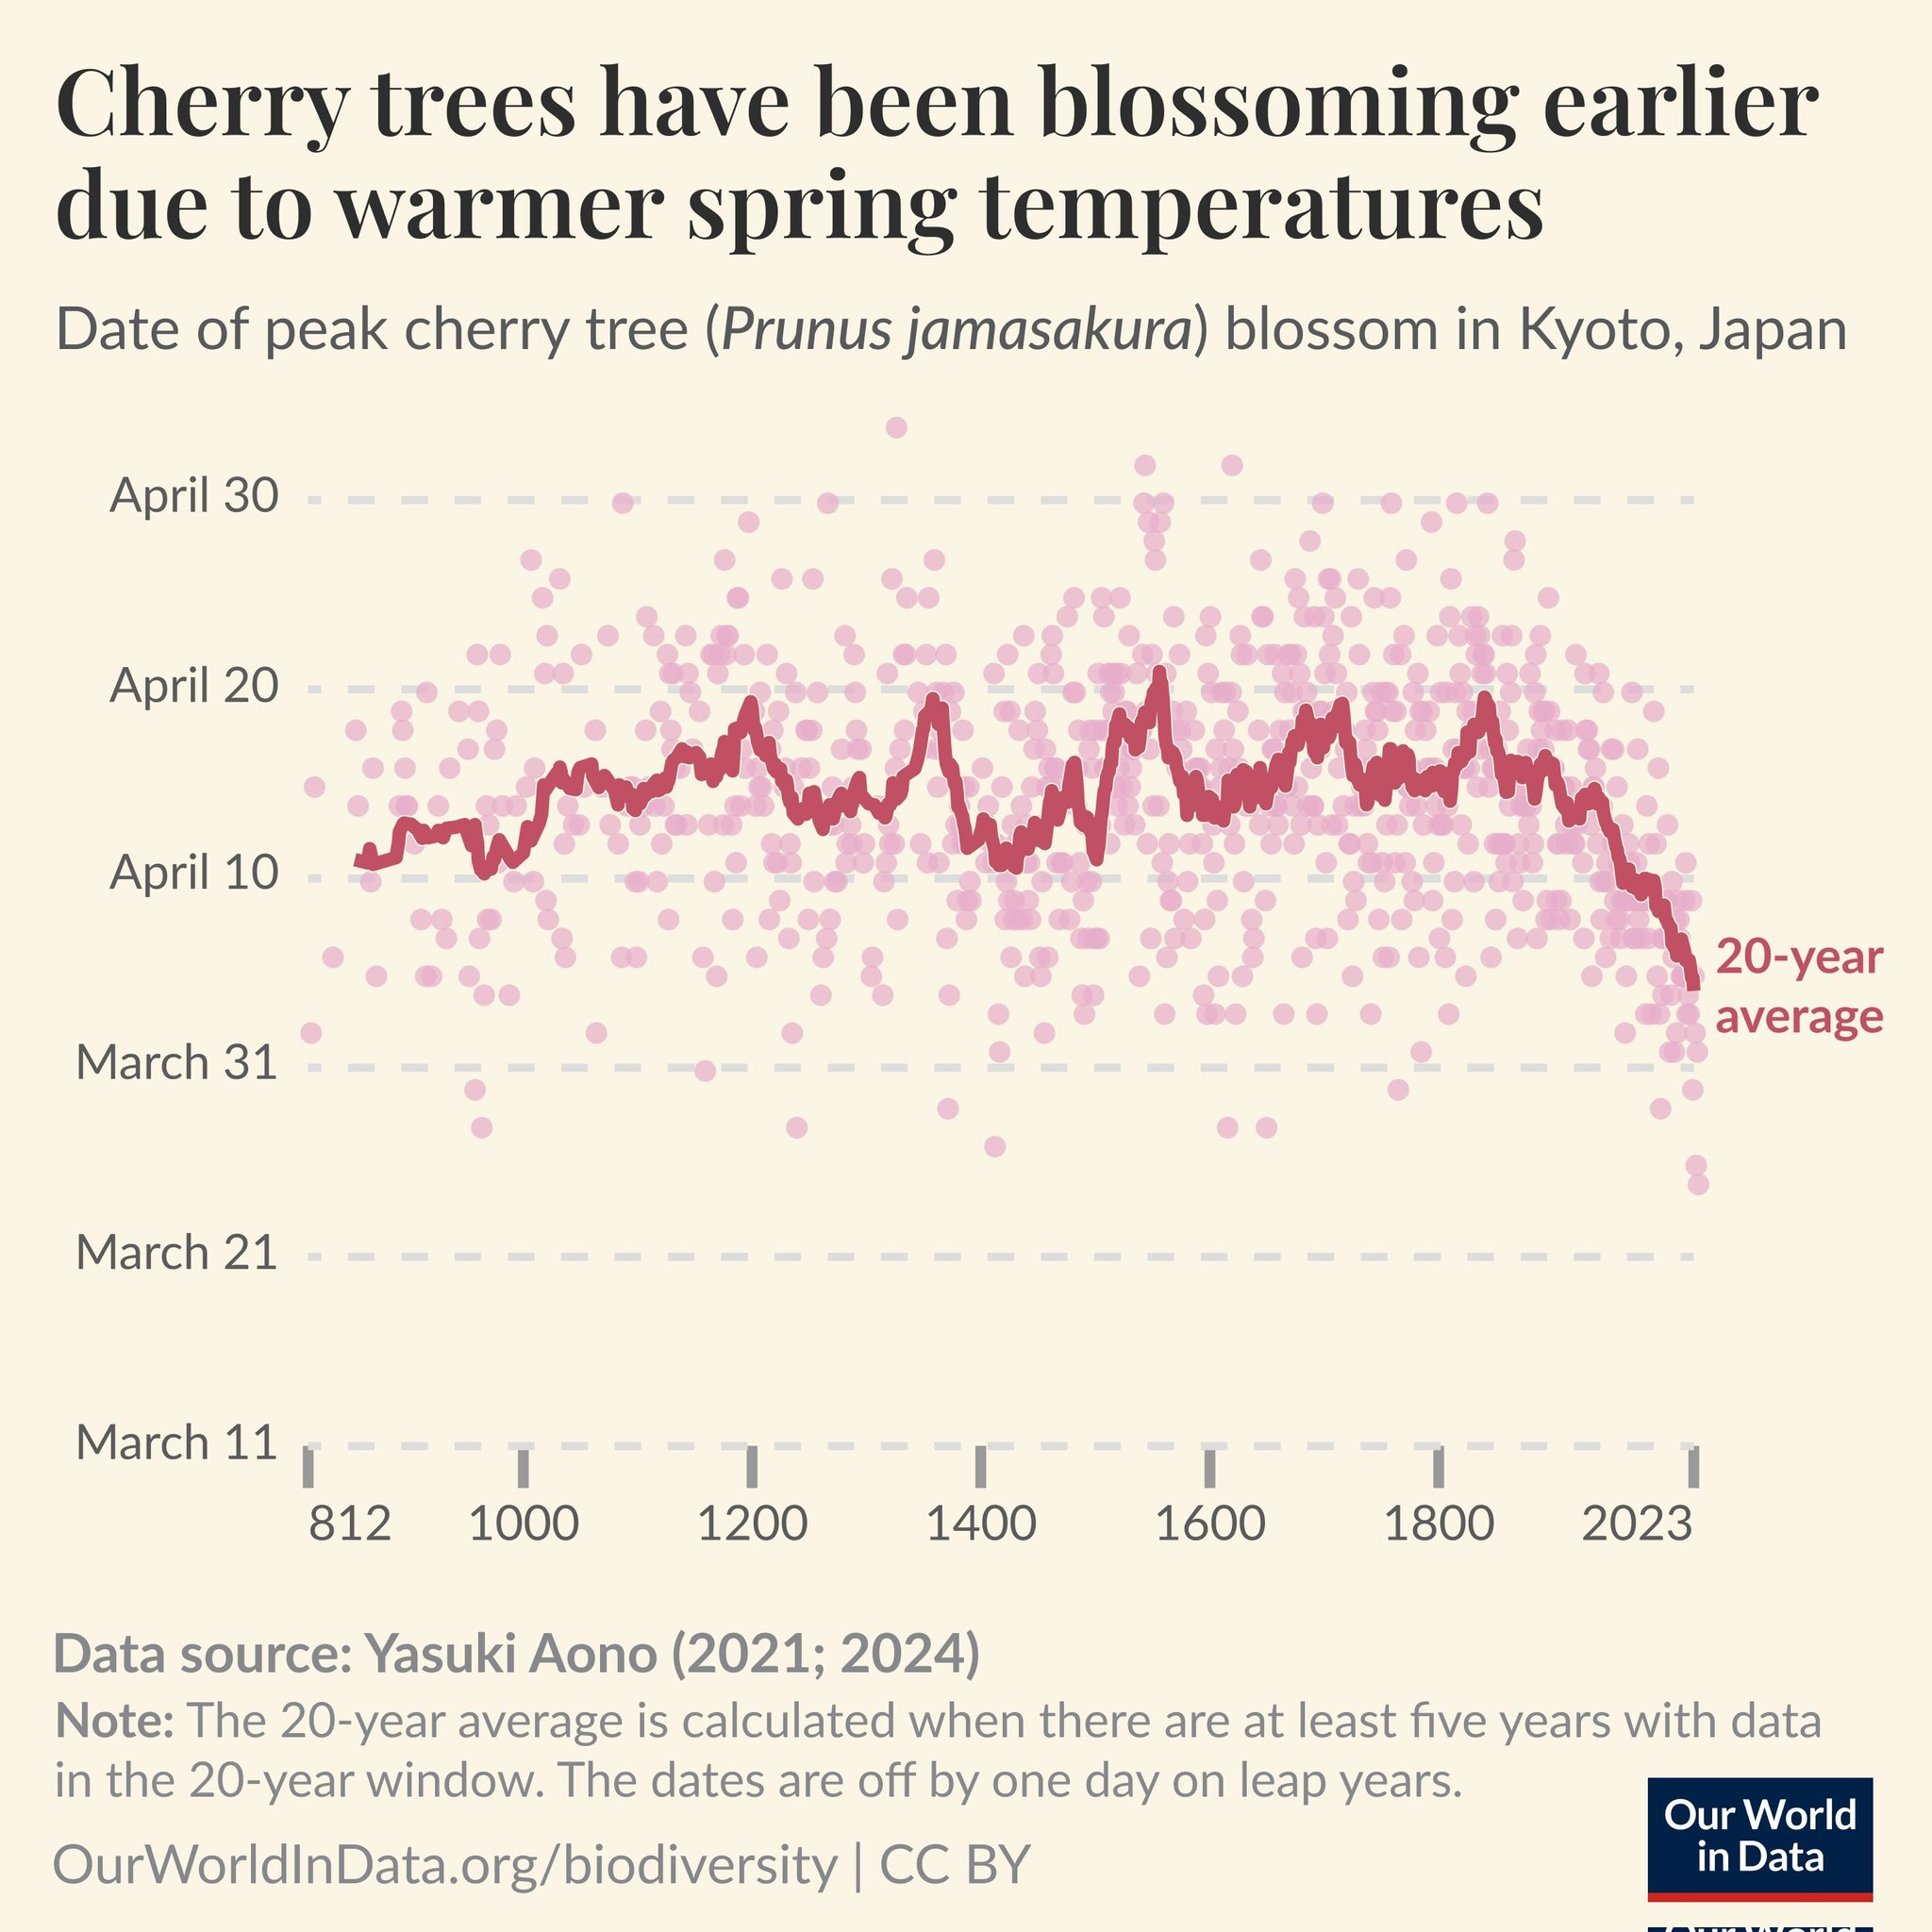
\includegraphics[height=.7\textheight]{cherry_blossoms.JPG}}
\only<8>{\centering\large Proximity and Distance\\~\\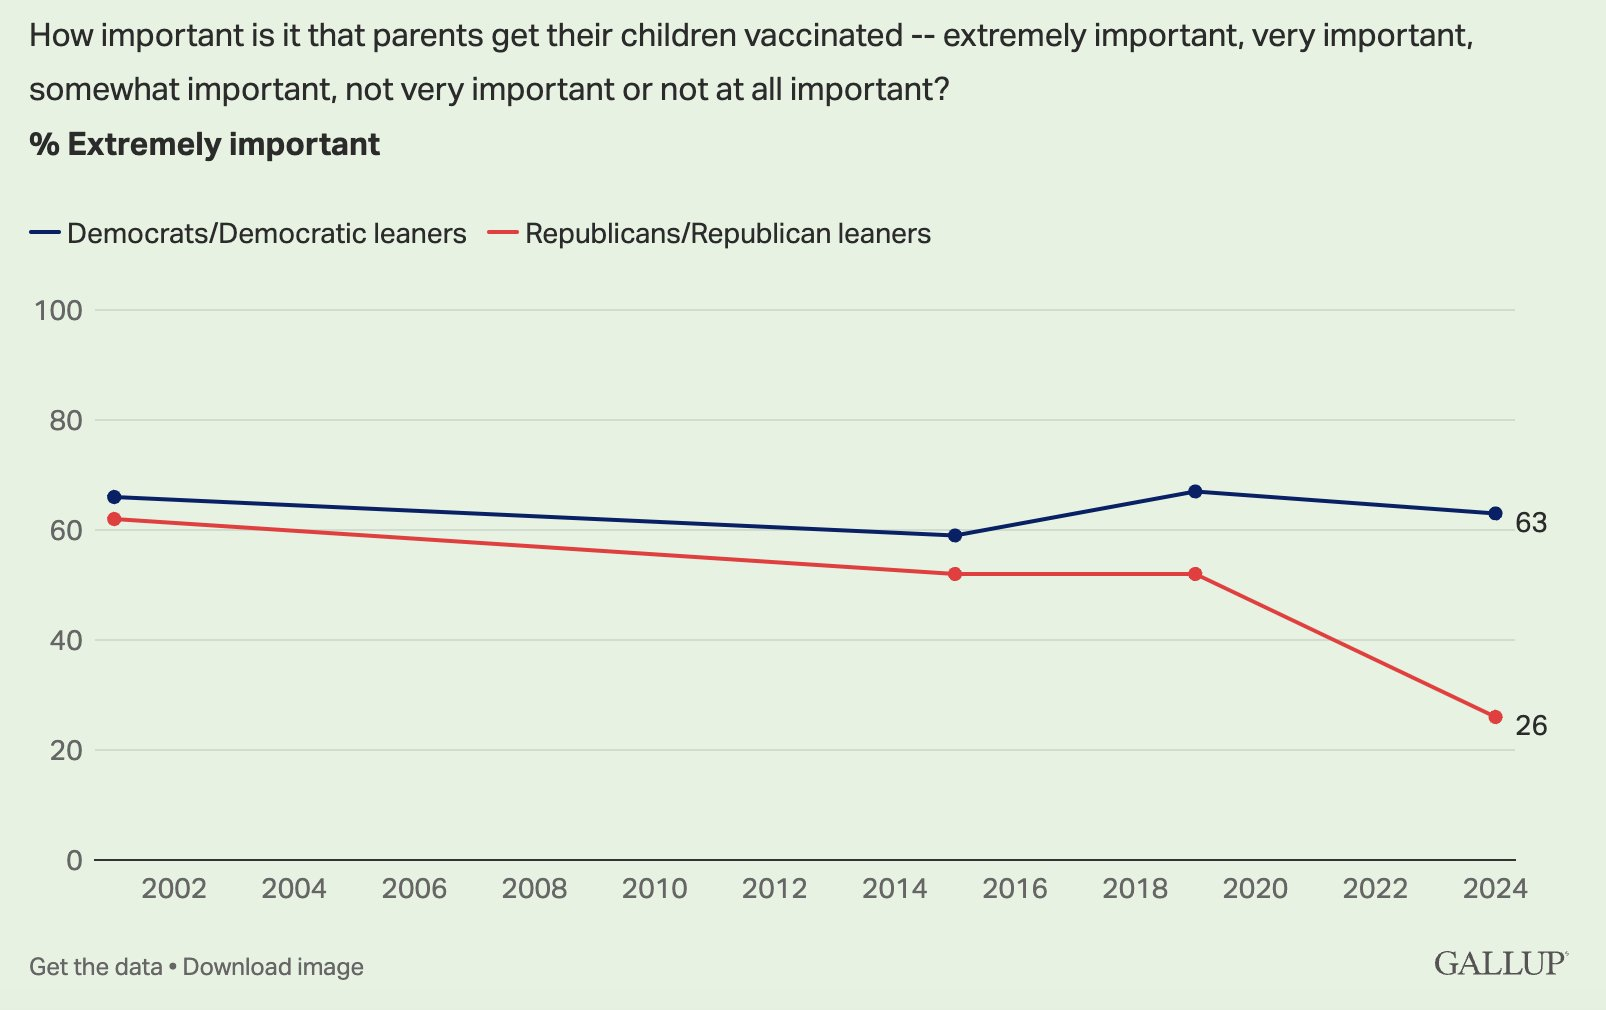
\includegraphics[height=.7\textheight]{vaccination.JPG}}
\only<9>{\centering\large Proximity and Distance\\~\\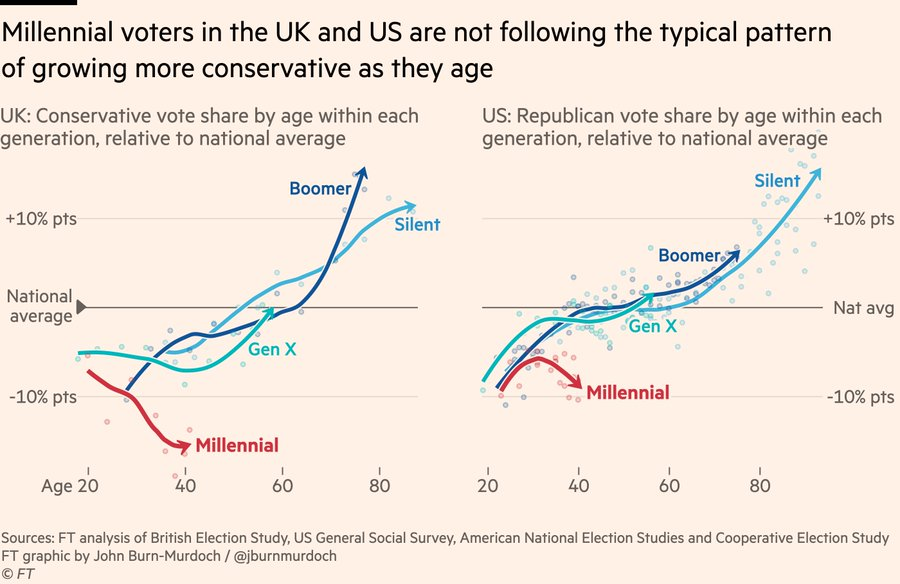
\includegraphics[height=.7\textheight]{ft_partisanship.PNG}}
\only<10>{\centering\large Similarity and Difference\\~\\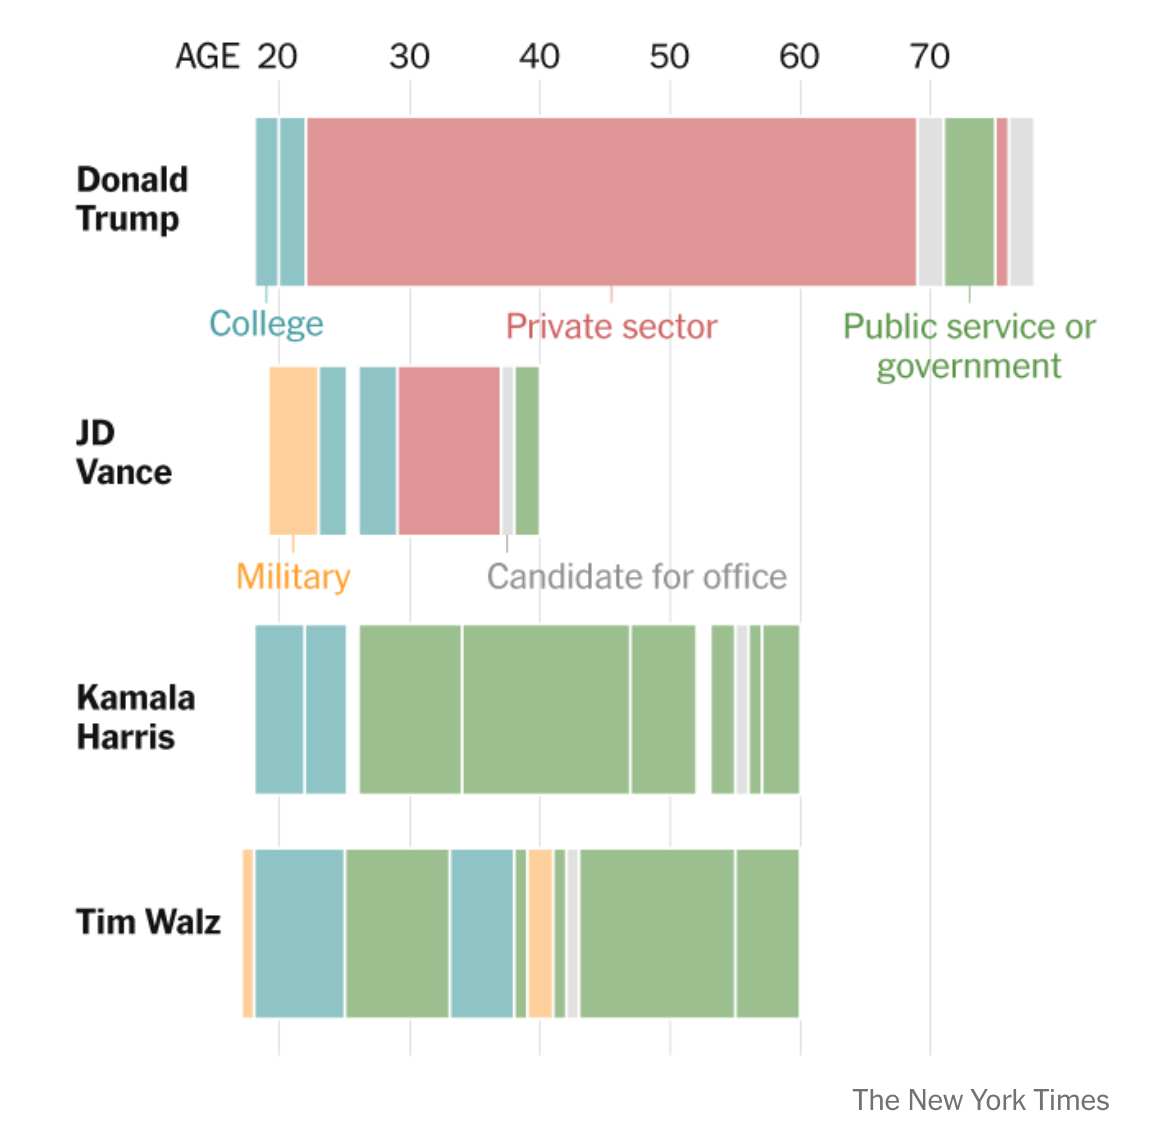
\includegraphics[height=.7\textheight]{nyt_candidate_histories.jpg}}
\only<11>{\centering\large Connectedness\\~\\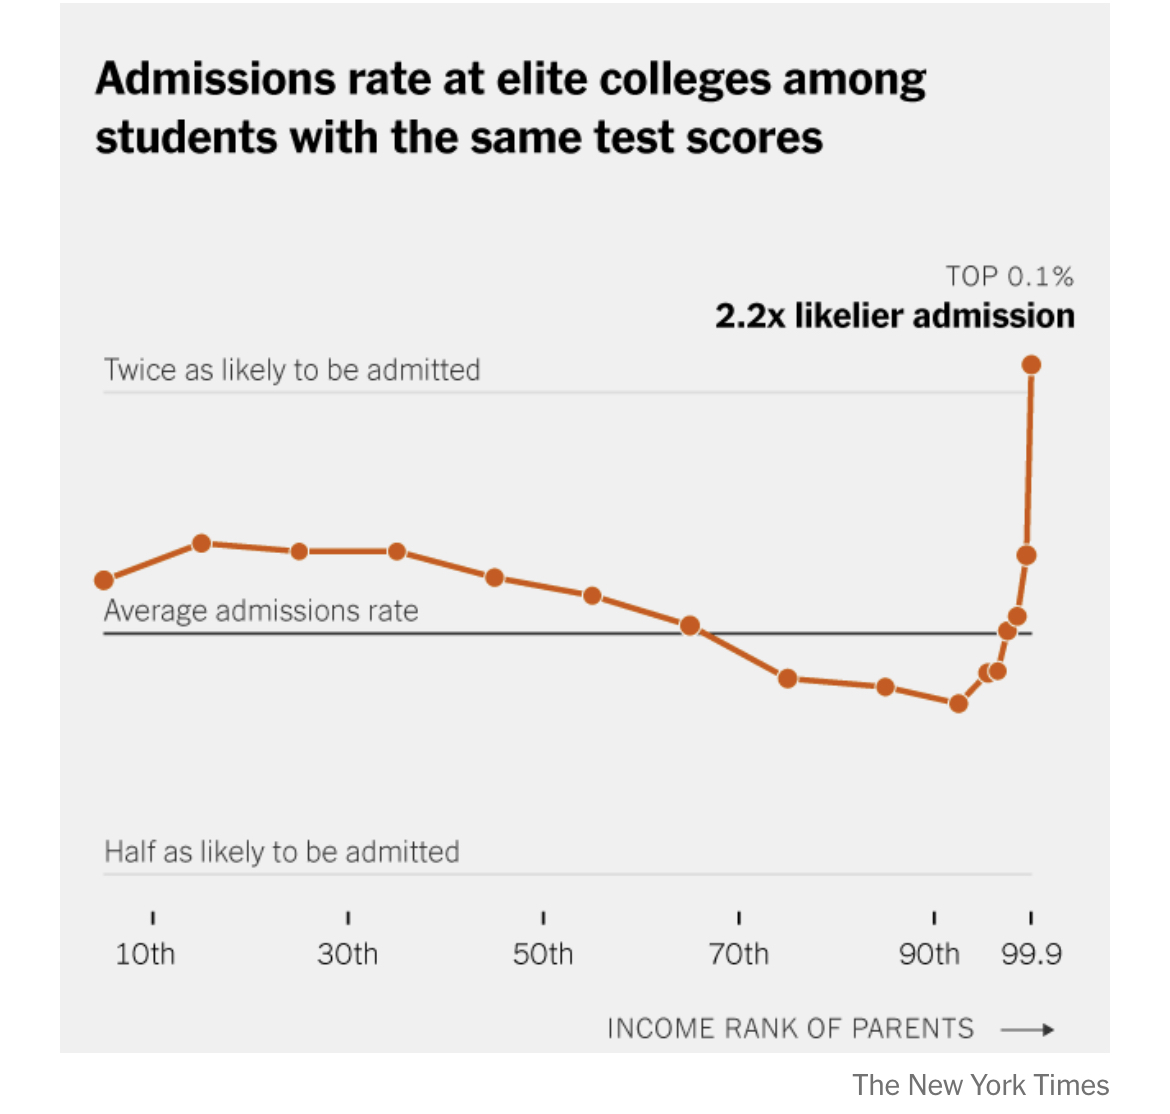
\includegraphics[height=.7\textheight]{nyt_admissions.jpg}}
\only<12>{\centering\large (Dis)Continuity\\~\\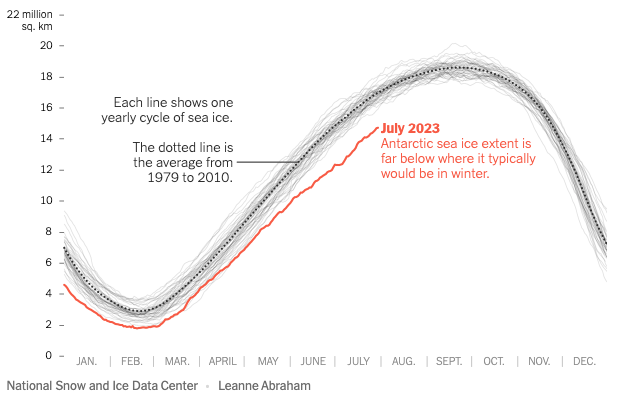
\includegraphics[height=.7\textheight]{nyt_antarctic_ice.png}}
\only<13>{\centering\large (Dis)Continuity\\~\\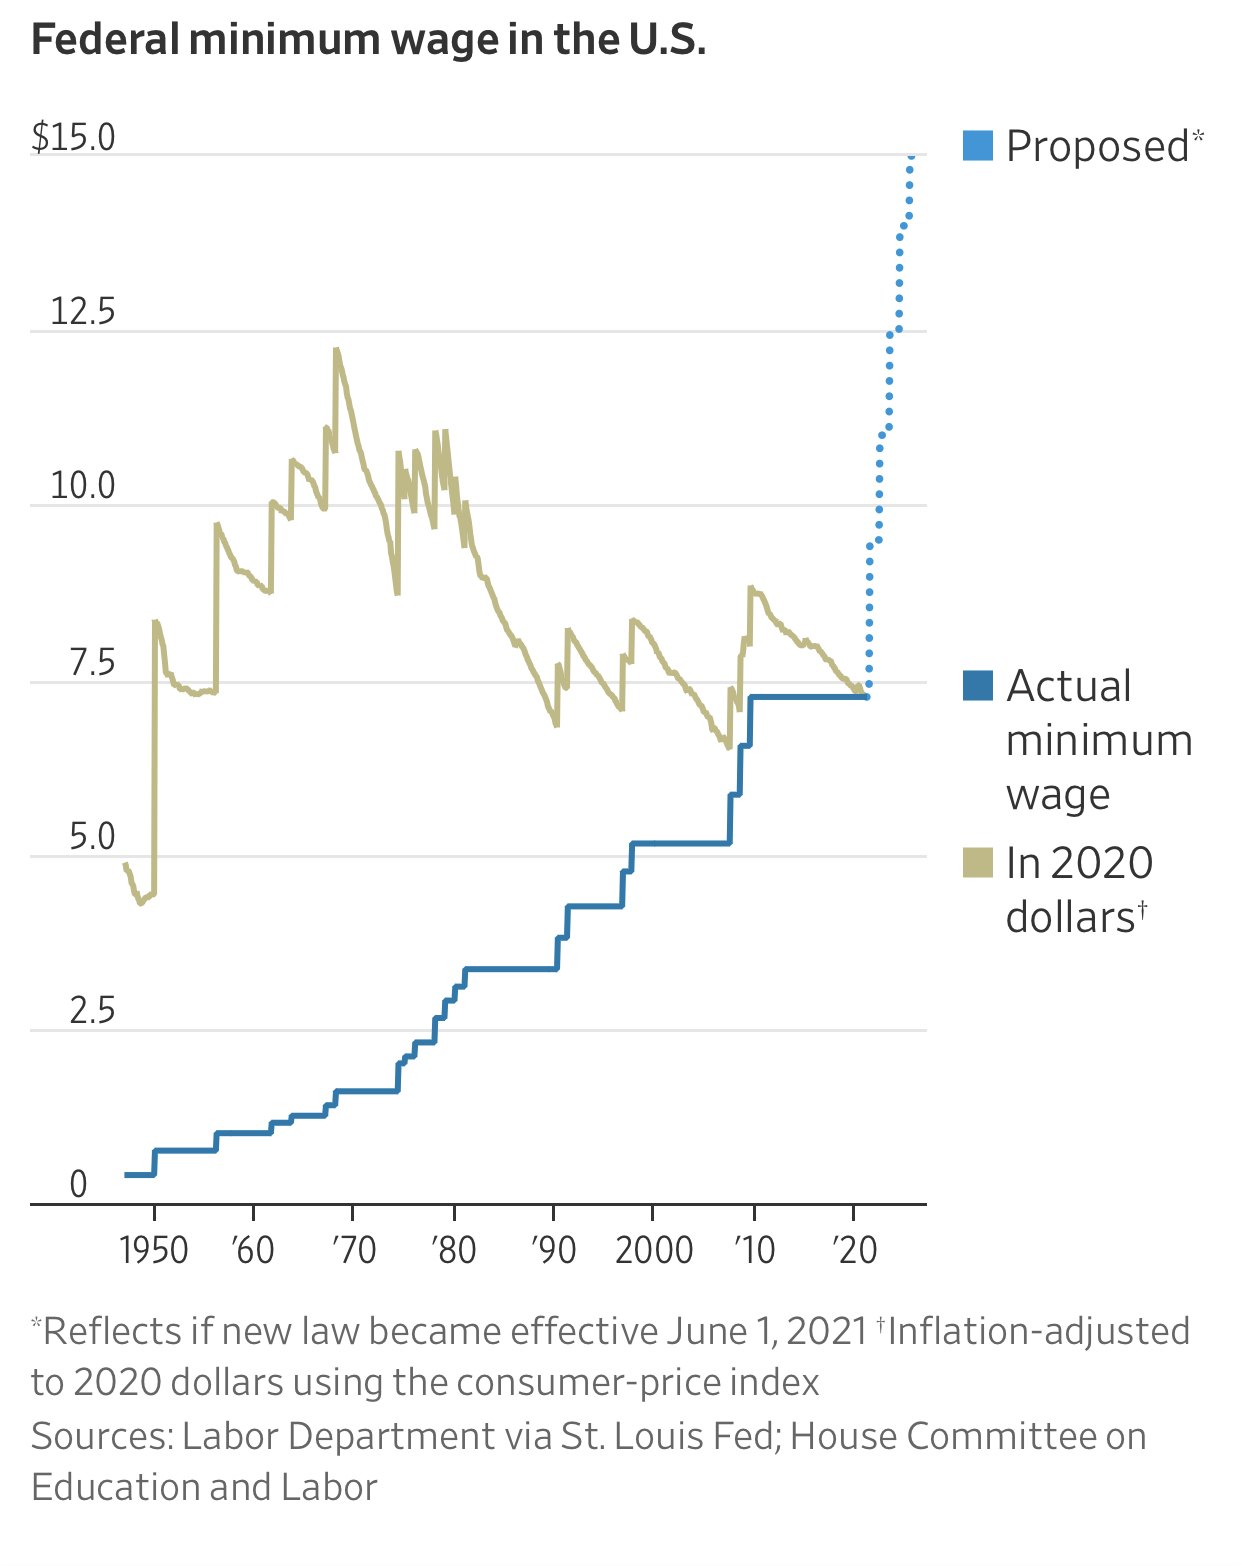
\includegraphics[height=.7\textheight]{wsj_minimum_wage.jpg}}
\only<14>{\centering\large Closure\\~\\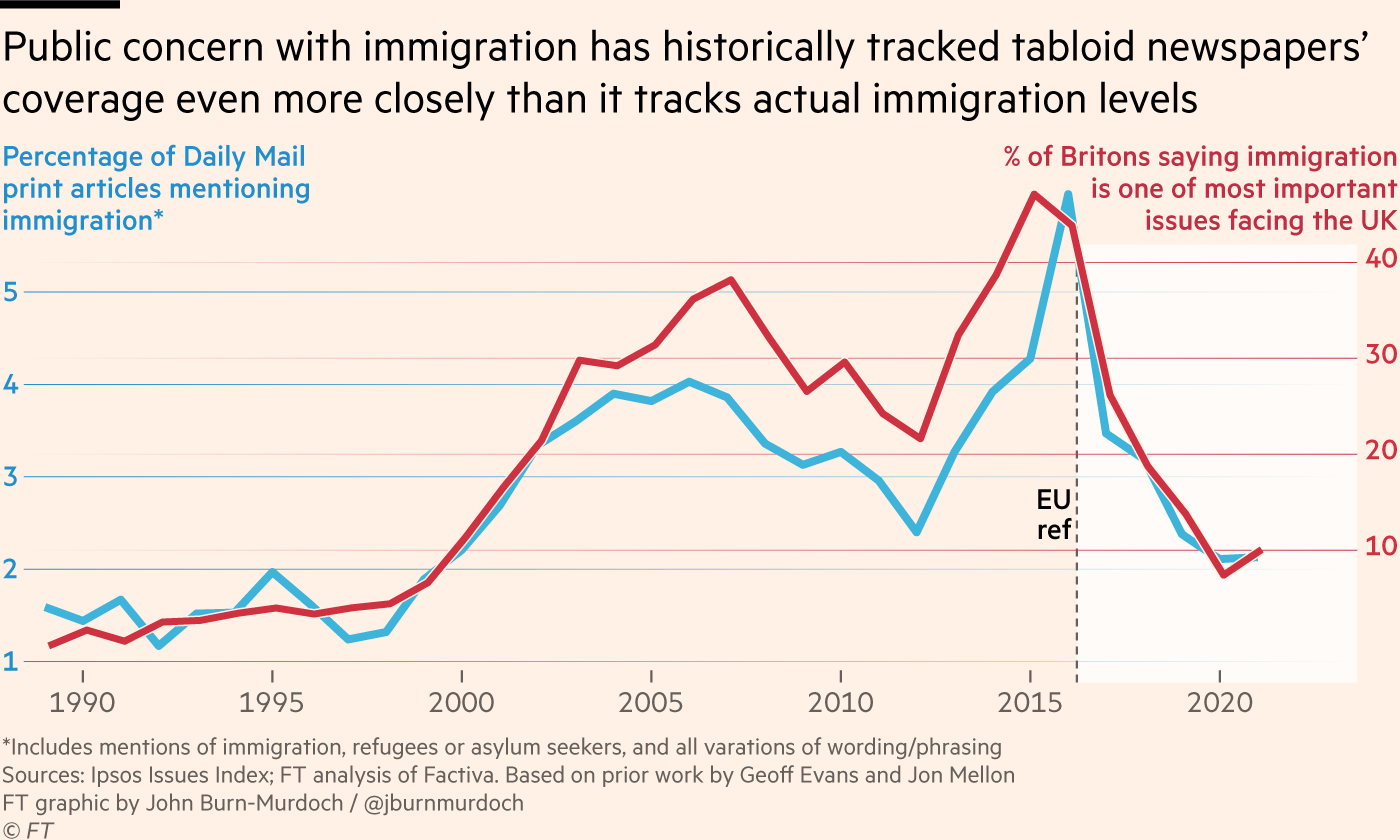
\includegraphics[height=.7\textheight]{ft_immigration.png}}
\only<15>{\centering\large Closure\\~\\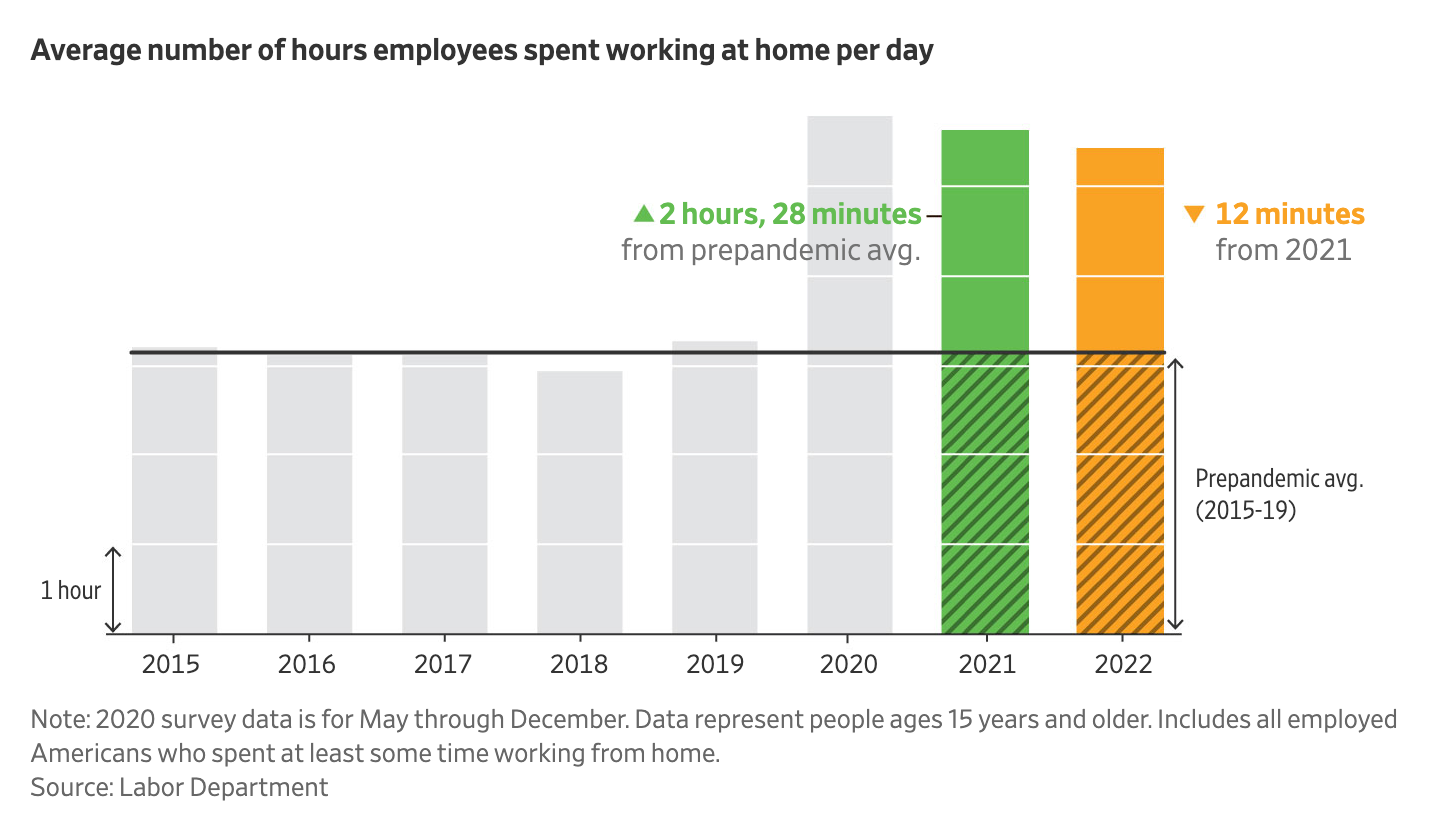
\includegraphics[height=.7\textheight]{wsj_wfh.png}}
\only<16>{\centering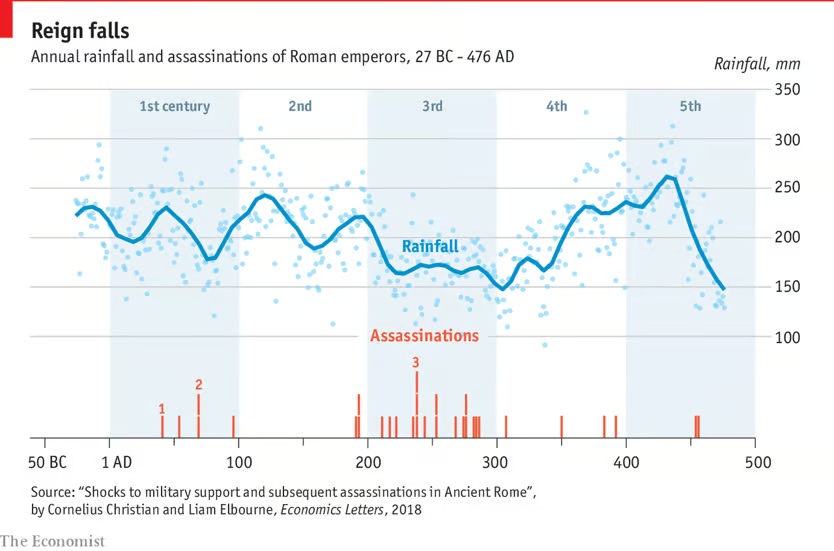
\includegraphics[width=.9\textwidth]{economist_assasinations.png}}
}

%%%%%%%%%%%%%%%%%%%%%%%%%%%%%%%%%%%%%%%%%%%%%%%%%%%%%%%%%%%%%%%%%%
\frame{\frametitle{Parts of a Graph}
    \centering
    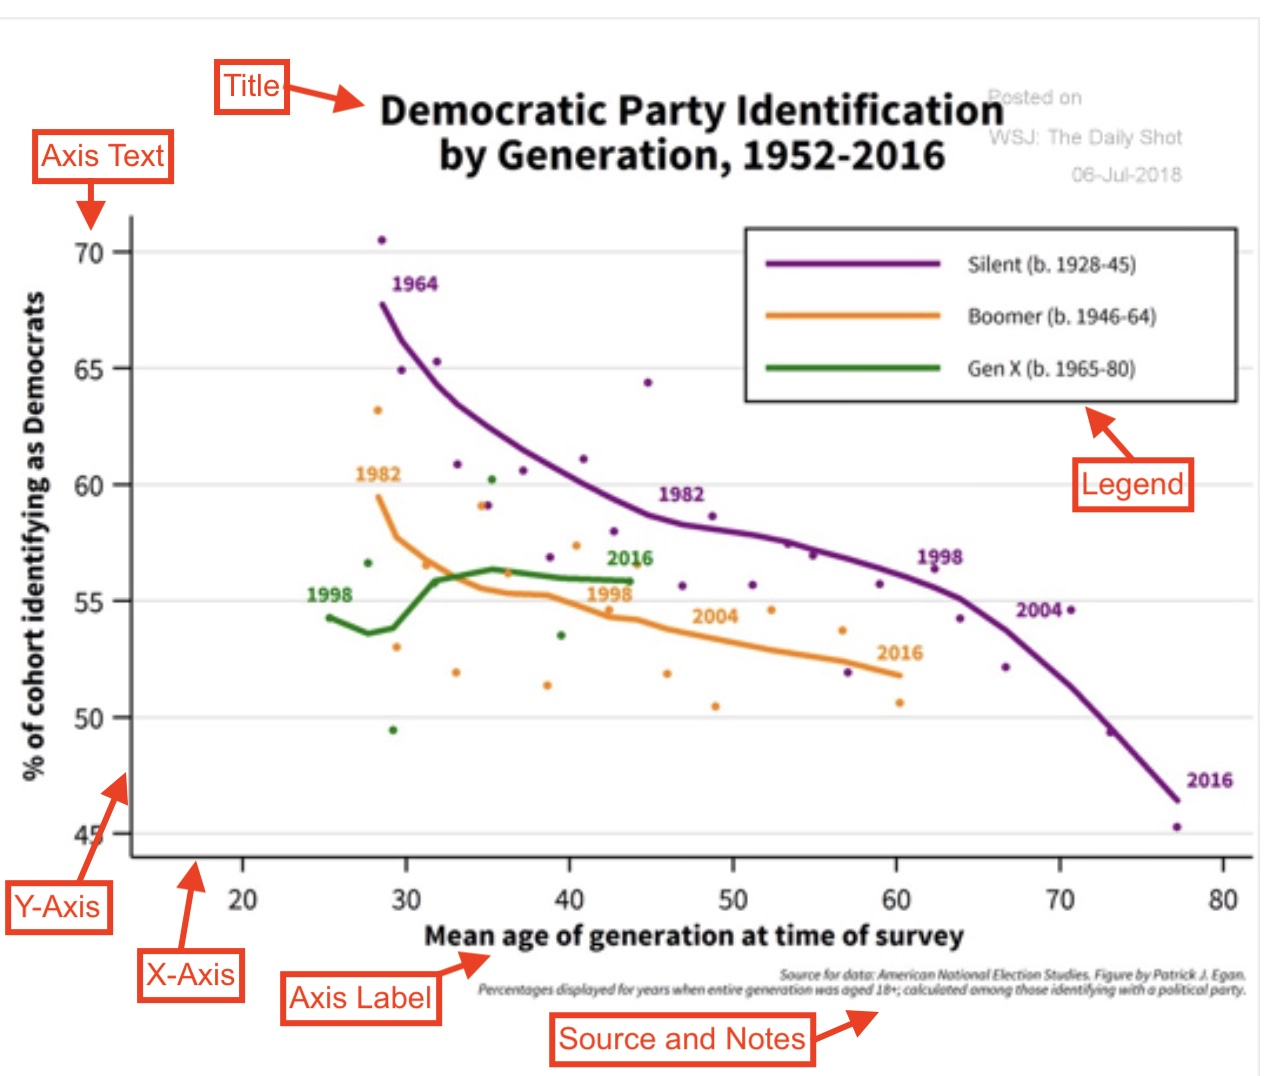
\includegraphics[width=.75\textwidth]{partsofgraph.jpg}
}

%%%%%%%%%%%%%%%%%%%%%%%%%%%%%%%%%%%%%%%%%%%%%%%%%%%%%%%%%%%%%%%%%%
\frame{\frametitle{Designing for Statistics}
\begin{columns}
\column{0.4\textwidth}
\begin{enumerate}[<+->]
        \item<1-> Show the context of the data
        \item<3-> The main axis should show the scale of the data
        \item<5-> Use conventional ordering and meanings
        \item<10-> Data visualizations are paragraphs about data
        \item<12-> Limit cognitive load
        \item<14-> No pie charts
        \item<15-> Not all data should be in a chart
    \end{enumerate}
\column{0.6\textwidth}
\centering
\only<1>{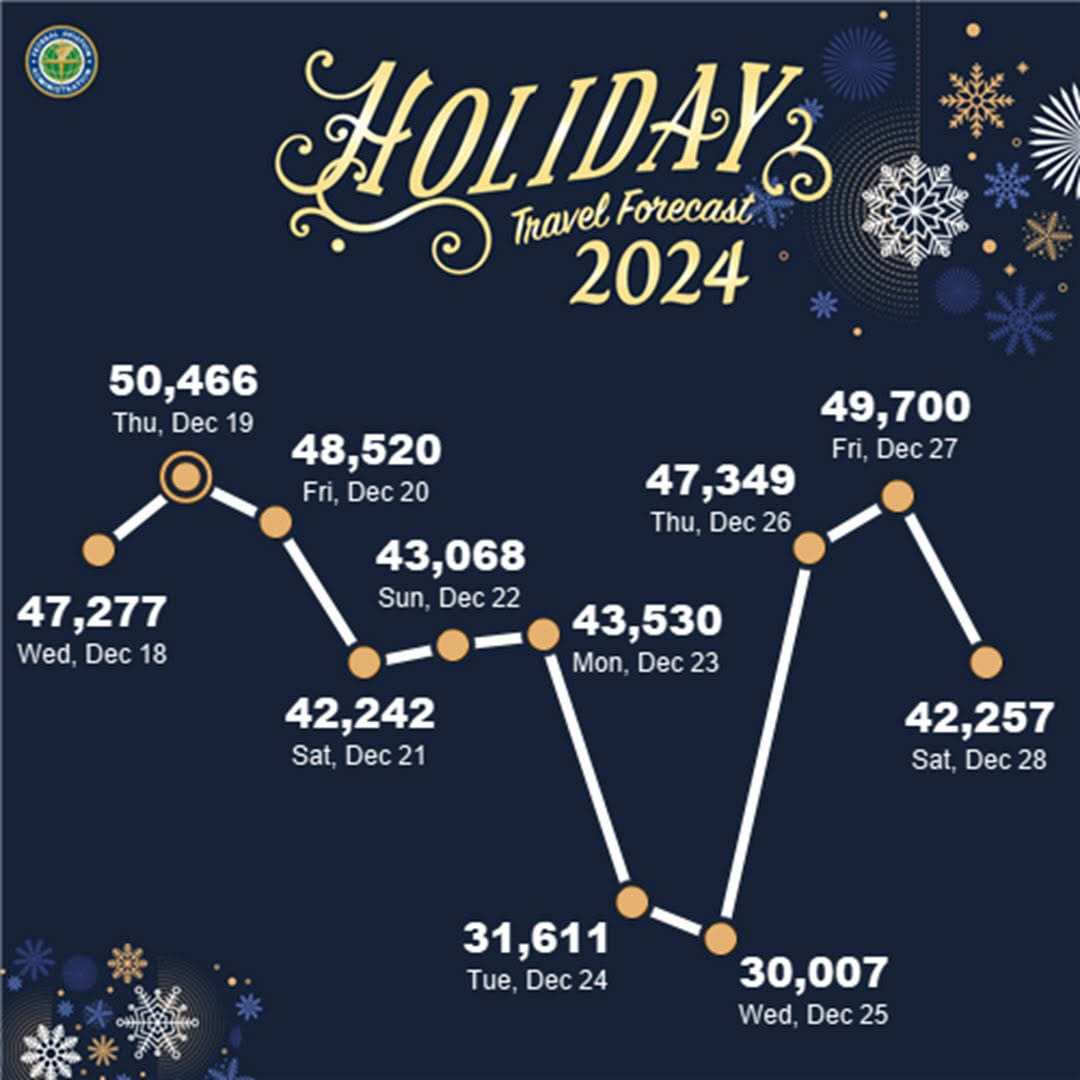
\includegraphics[width=\textwidth]{holiday_travel.jpg}}
\only<2>{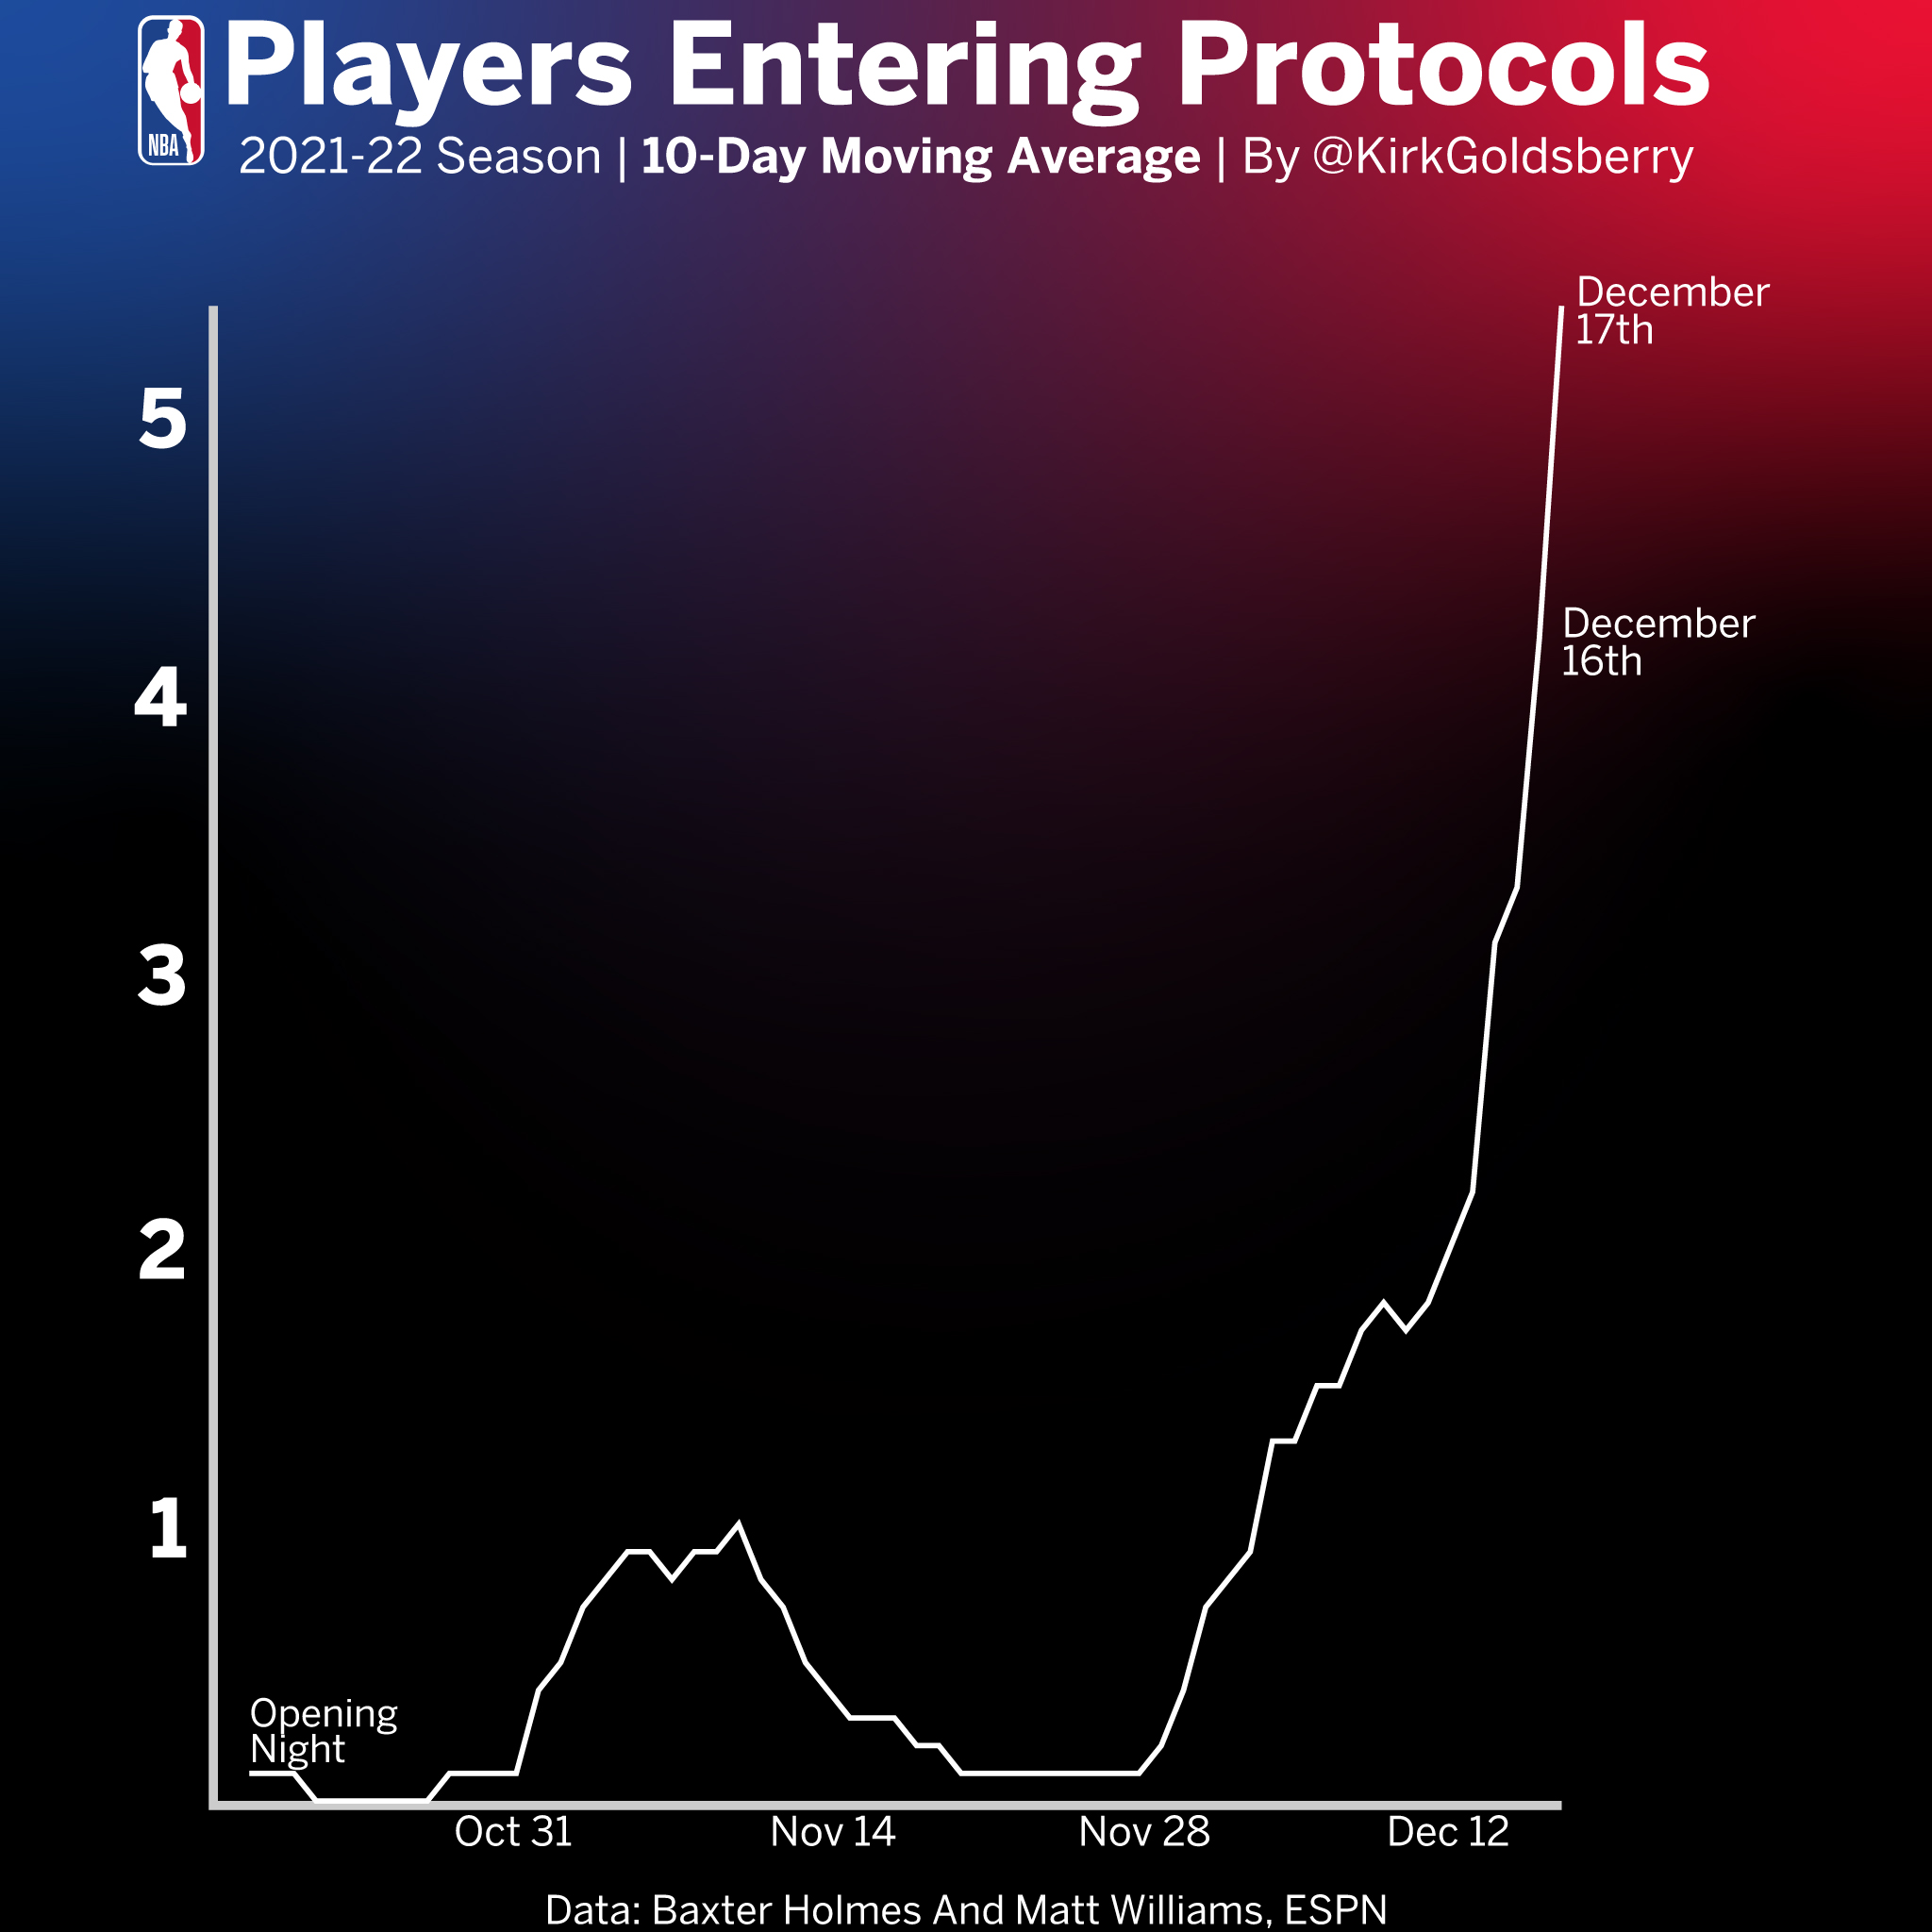
\includegraphics[width=\textwidth]{nba_covid.jpg}}
\only<3>{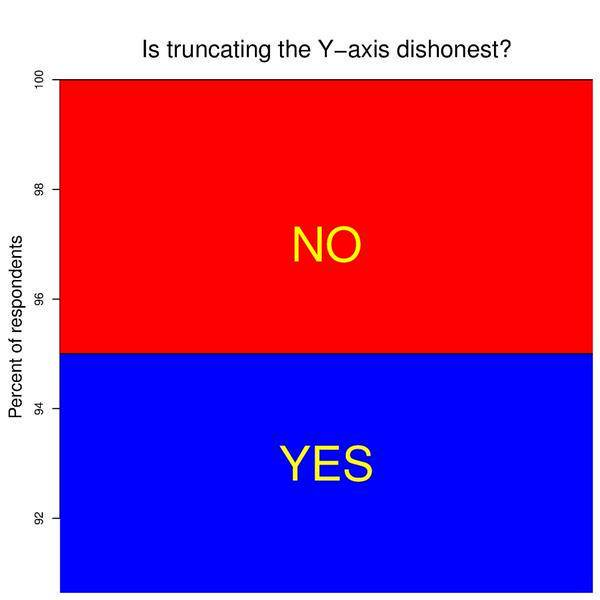
\includegraphics[width=\textwidth]{truncated_y_axis.jpeg}}
\only<4>{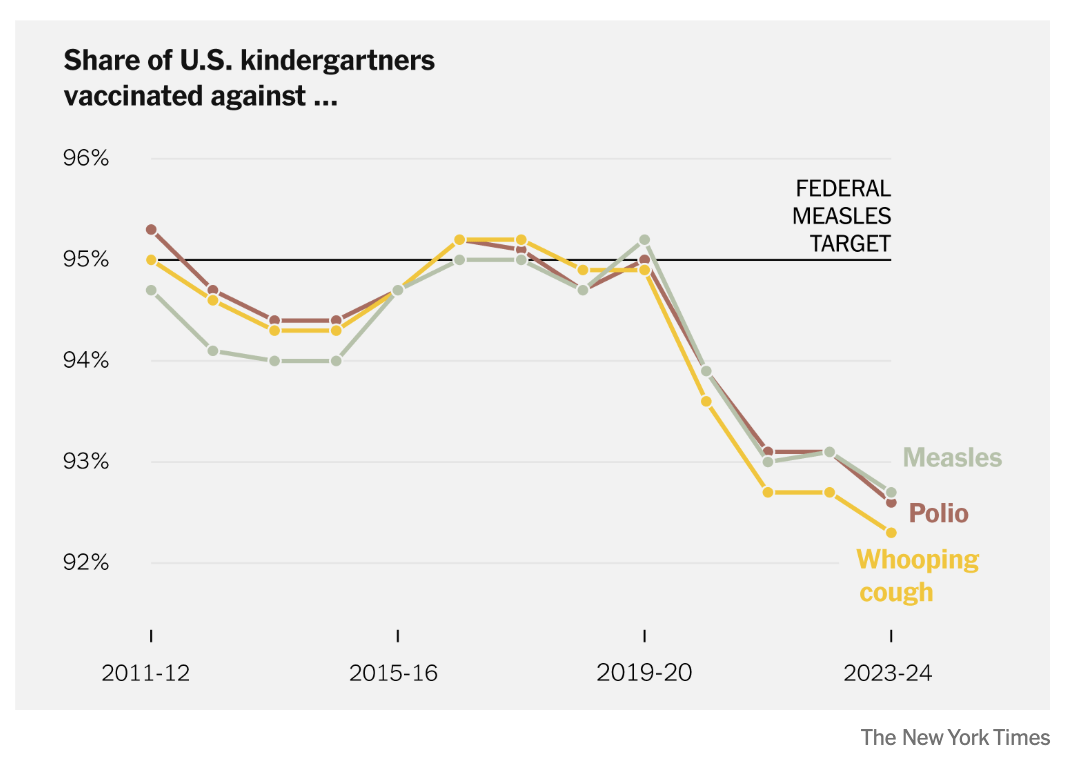
\includegraphics[width=\textwidth]{nyt_vaccination.png}}
\only<5>{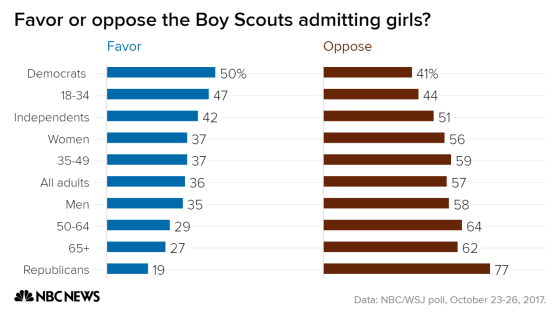
\includegraphics[width=\textwidth]{nbc_boy_scouts.png}}
\only<6>{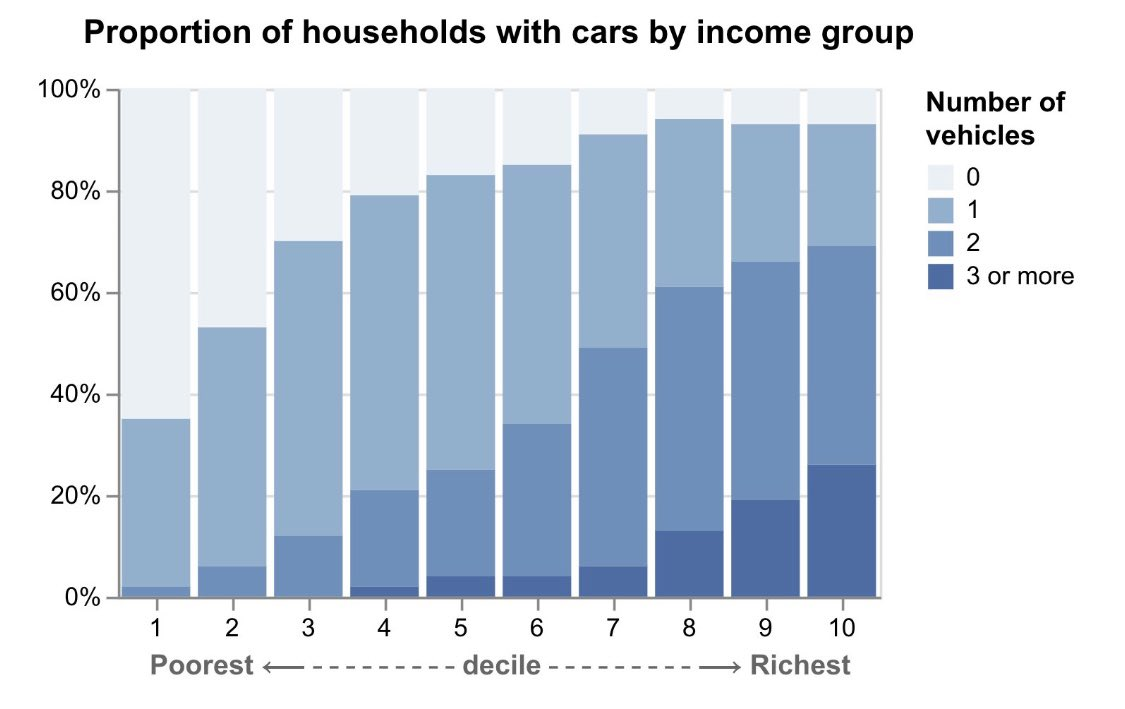
\includegraphics[width=\textwidth]{vehicles_by_income.jpg}}
\only<7>{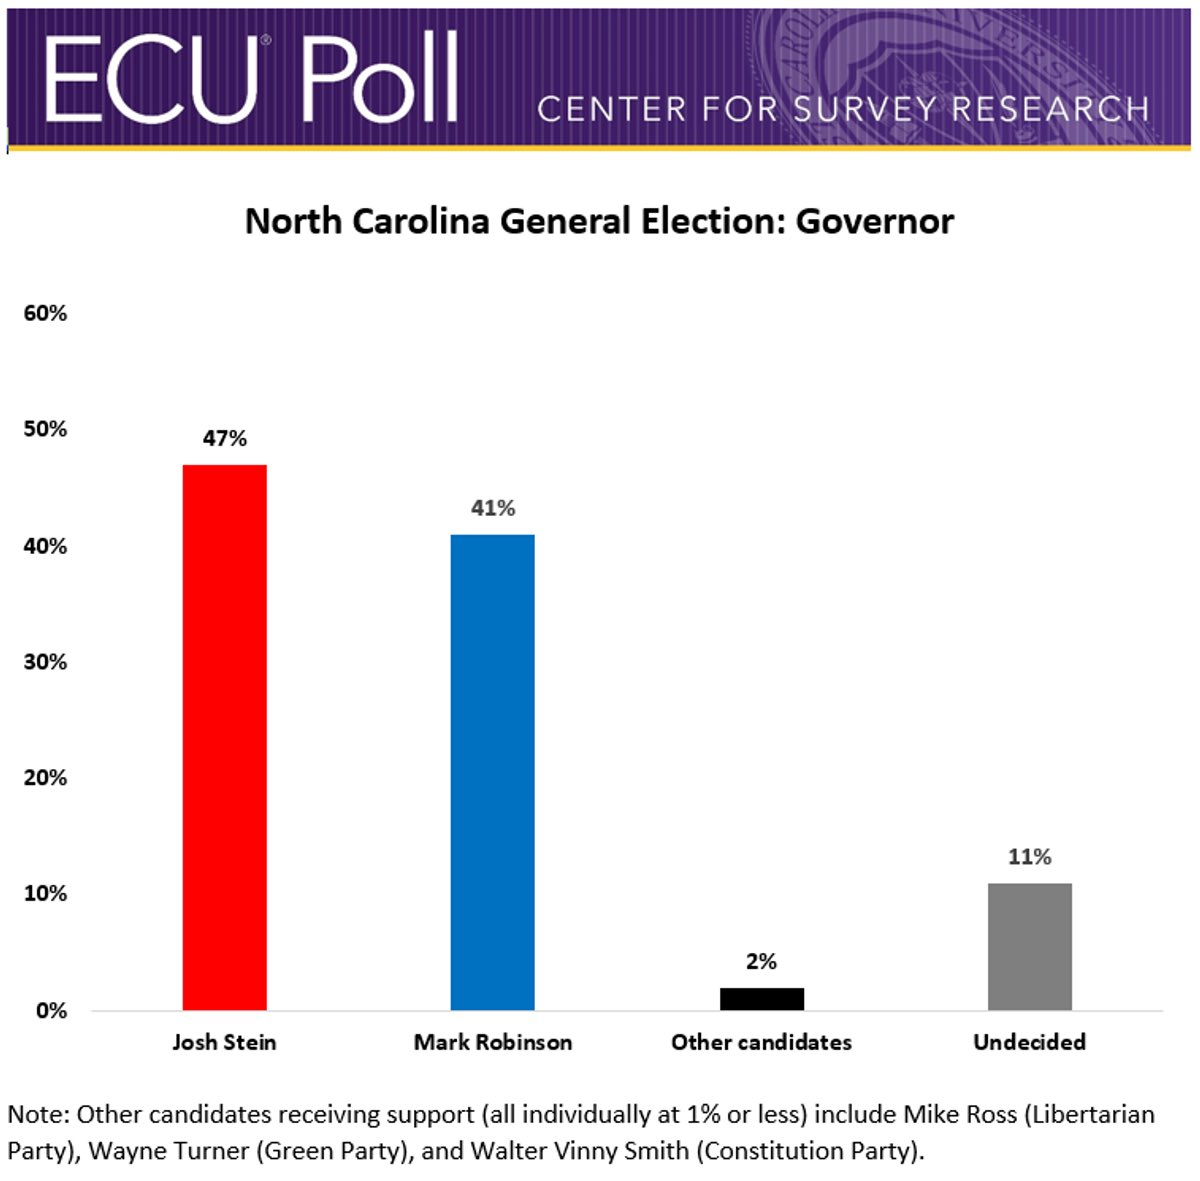
\includegraphics[width=\textwidth]{stein_robinson_poll.jpeg}}
\only<8>{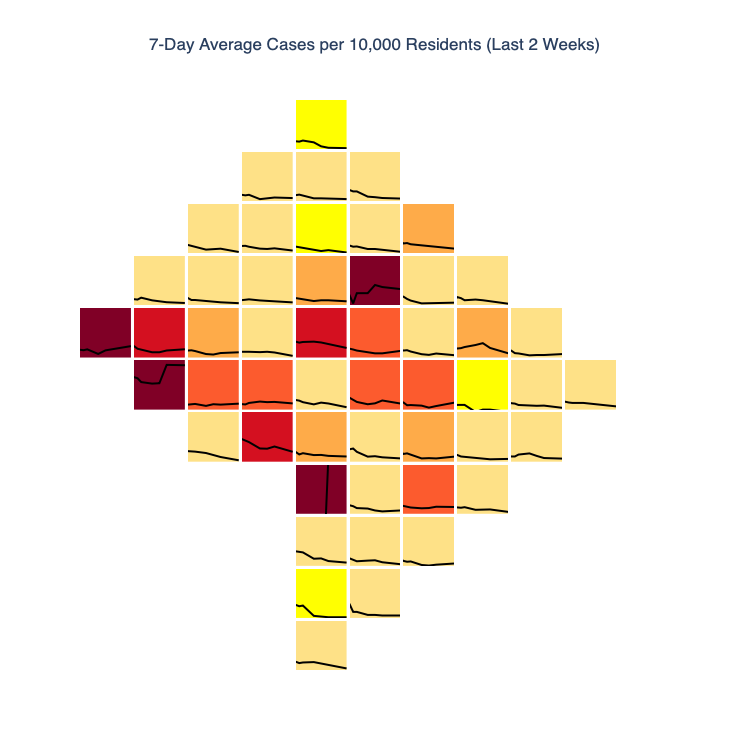
\includegraphics[width=\textwidth]{DC_covid.png}}
\only<9>{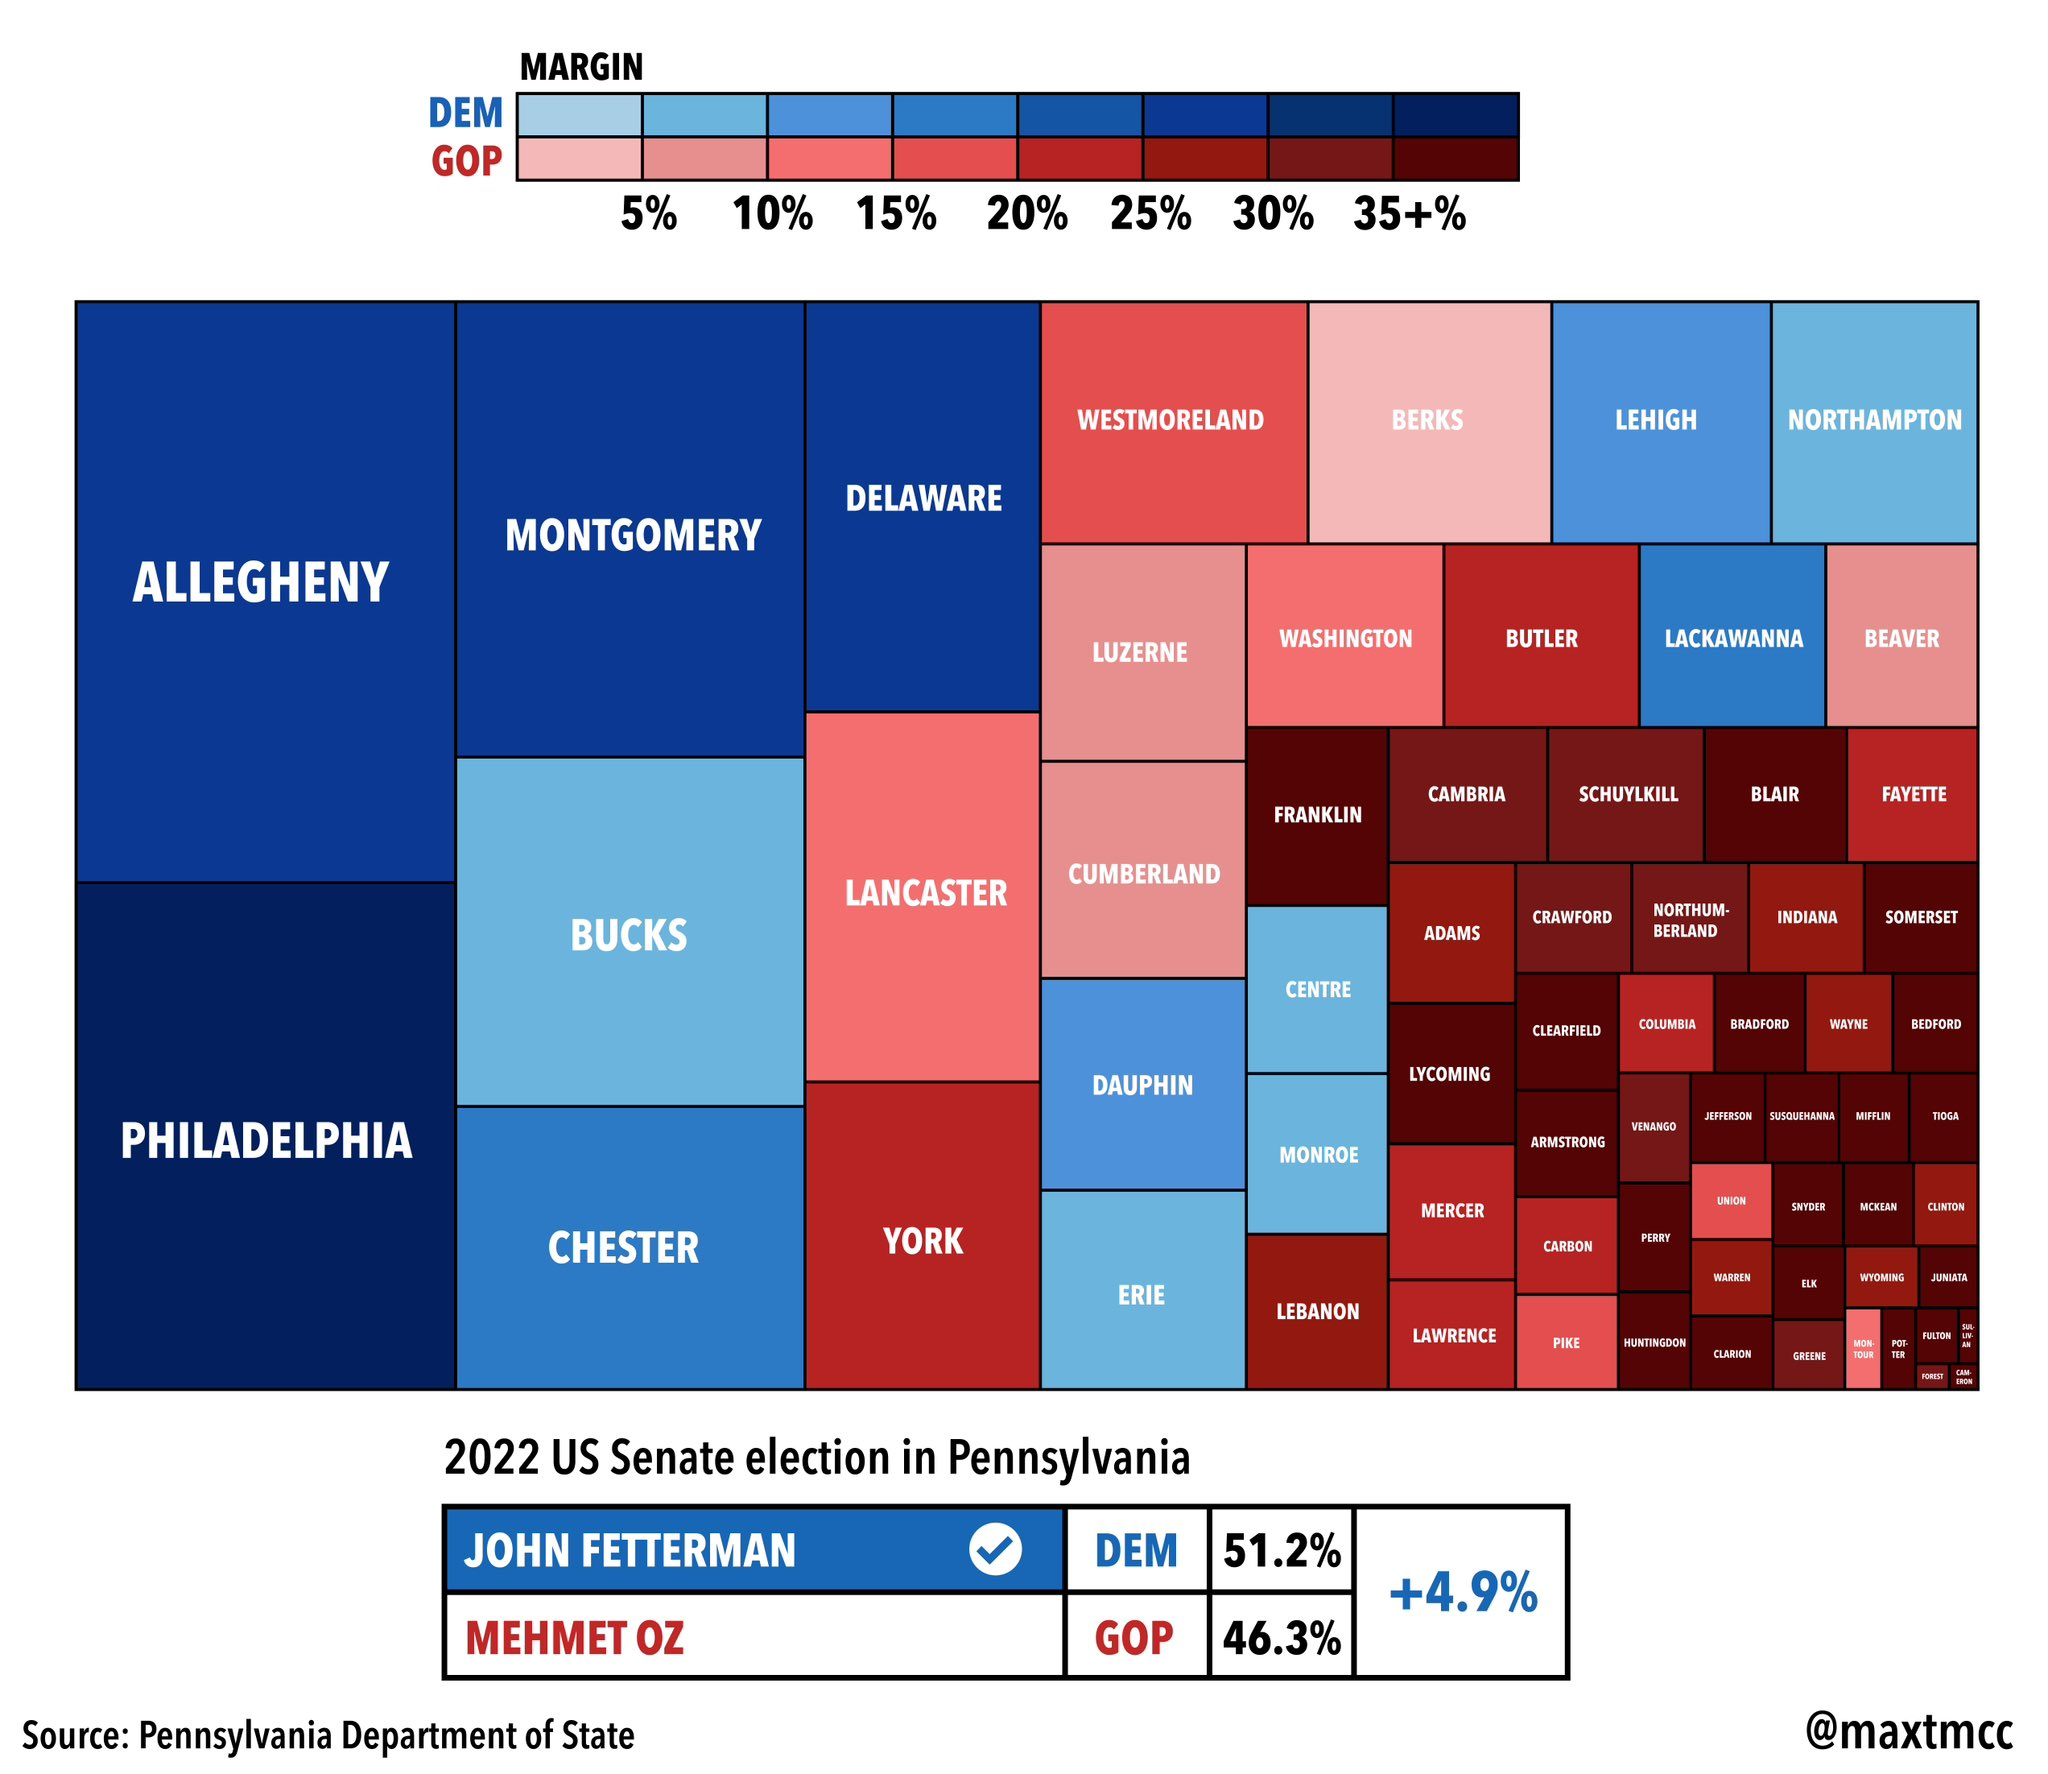
\includegraphics[width=\textwidth]{pa_sen_result.JPG}}
\only<10>{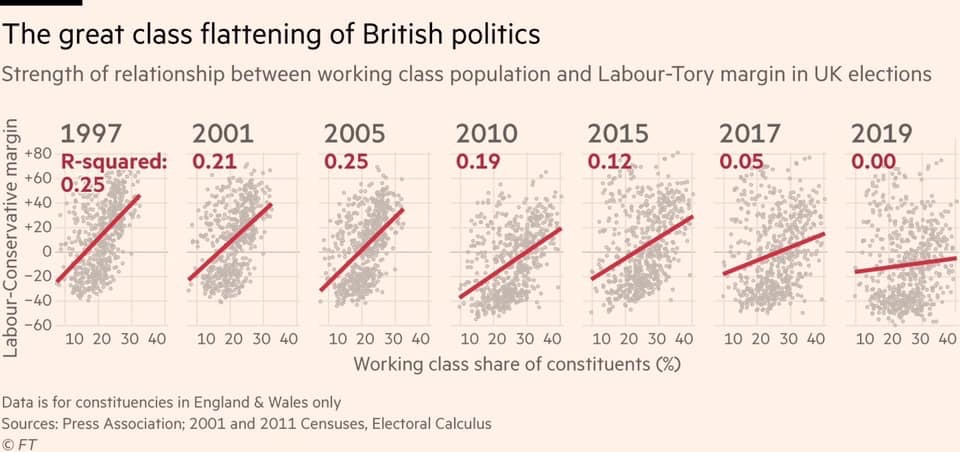
\includegraphics[width=\textwidth]{ft_britishpolit.JPG}}
\only<11>{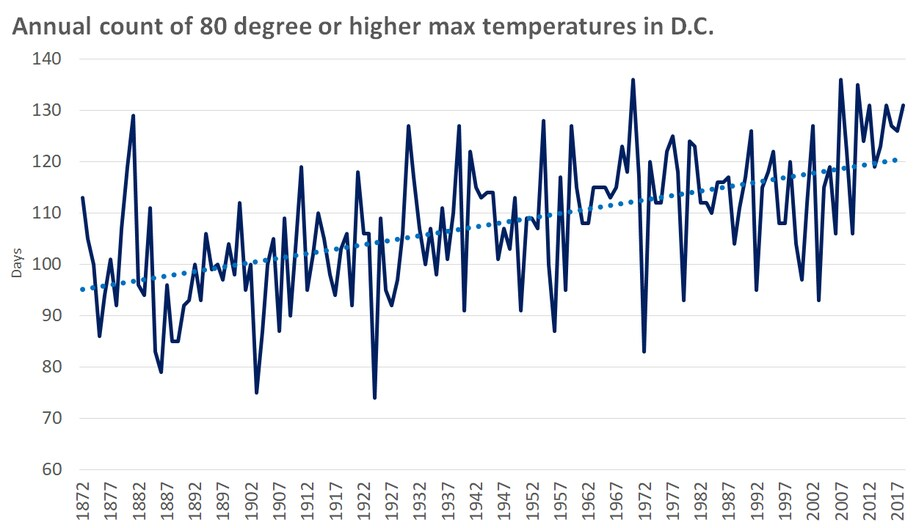
\includegraphics[width=\textwidth]{wapo_80_degrees.jpeg}}
\only<12>{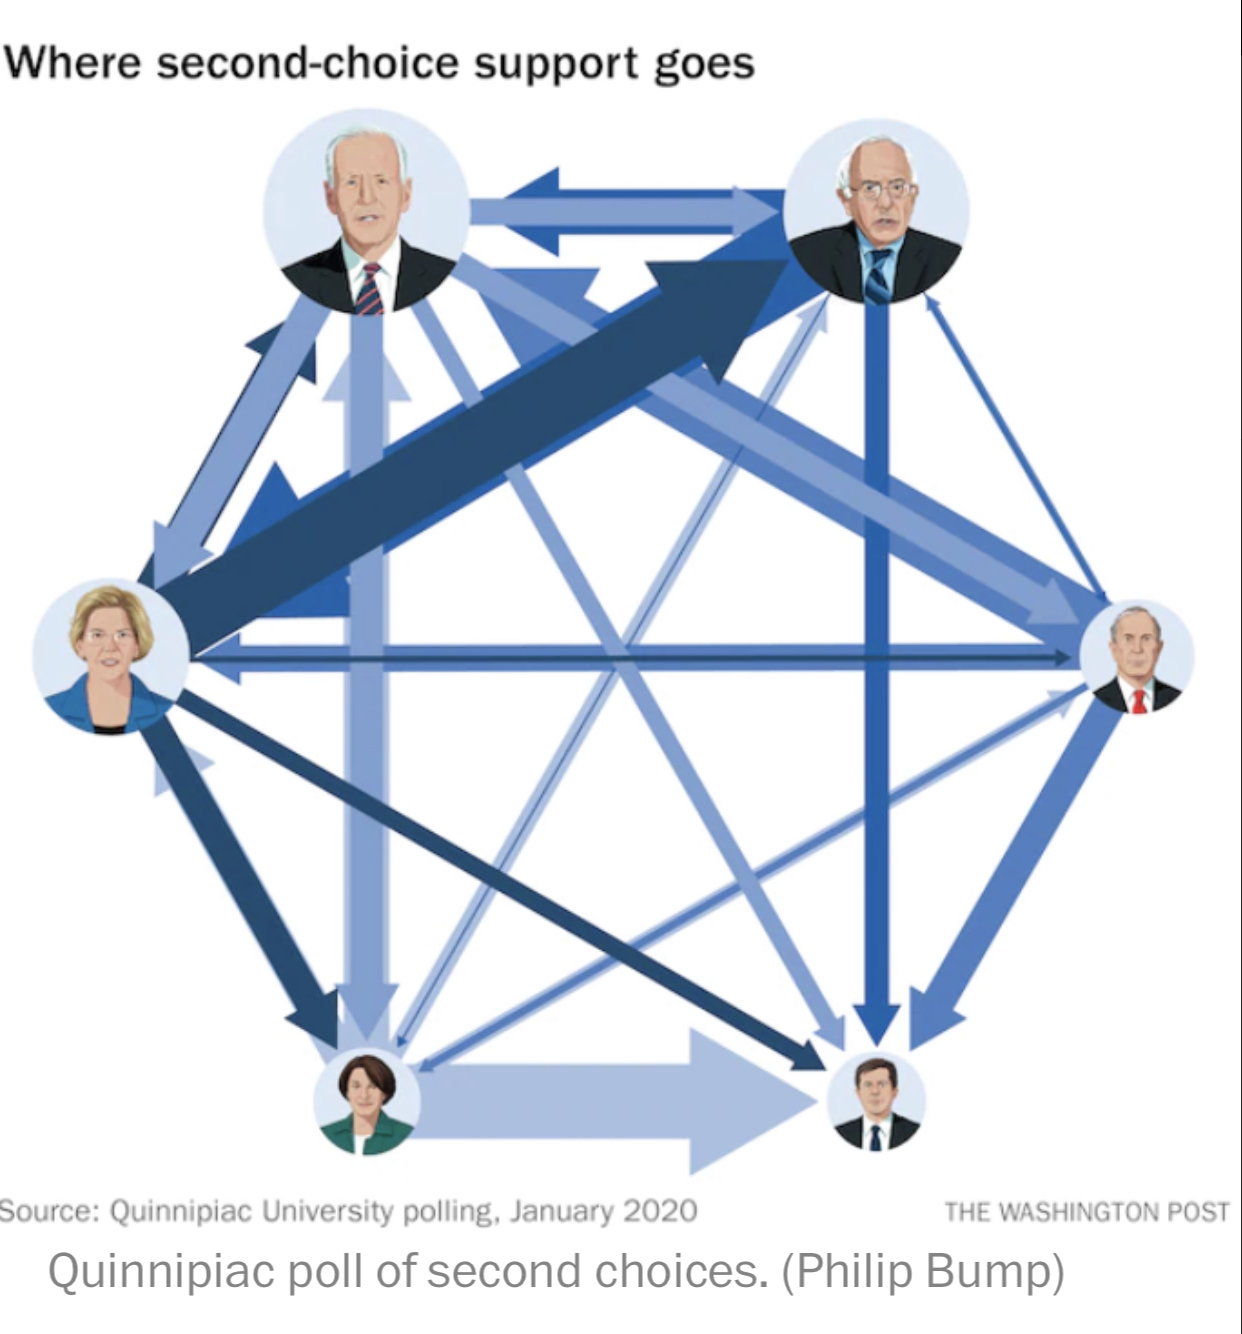
\includegraphics[width=\textwidth]{wapo_second_choices.jpg}}
\only<13>{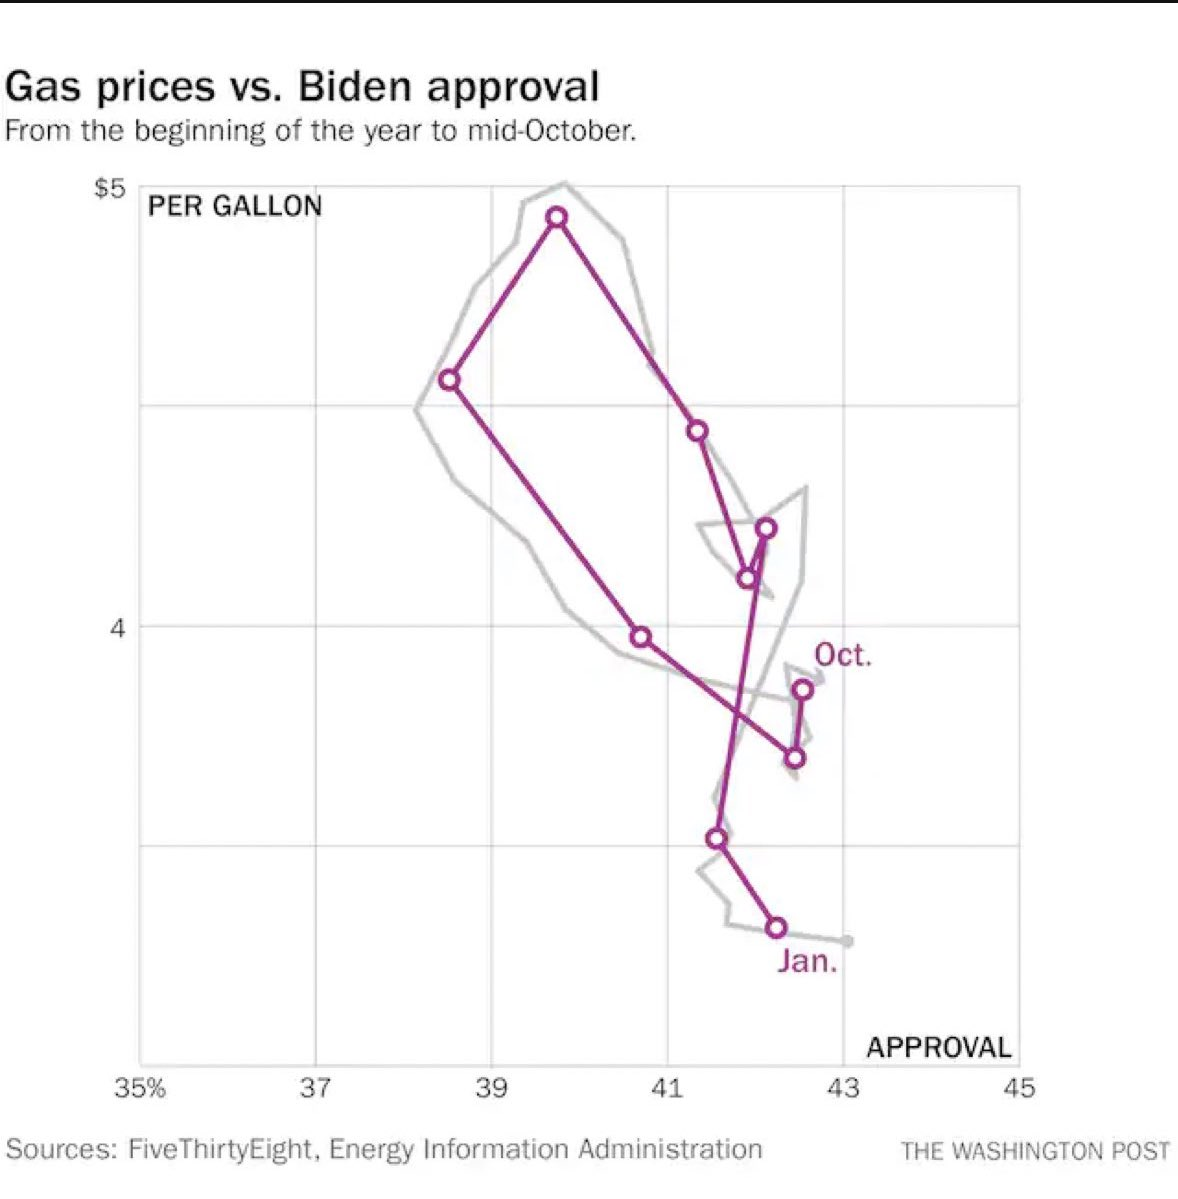
\includegraphics[width=\textwidth]{wapo_gas_prices.JPG}}
\only<14>{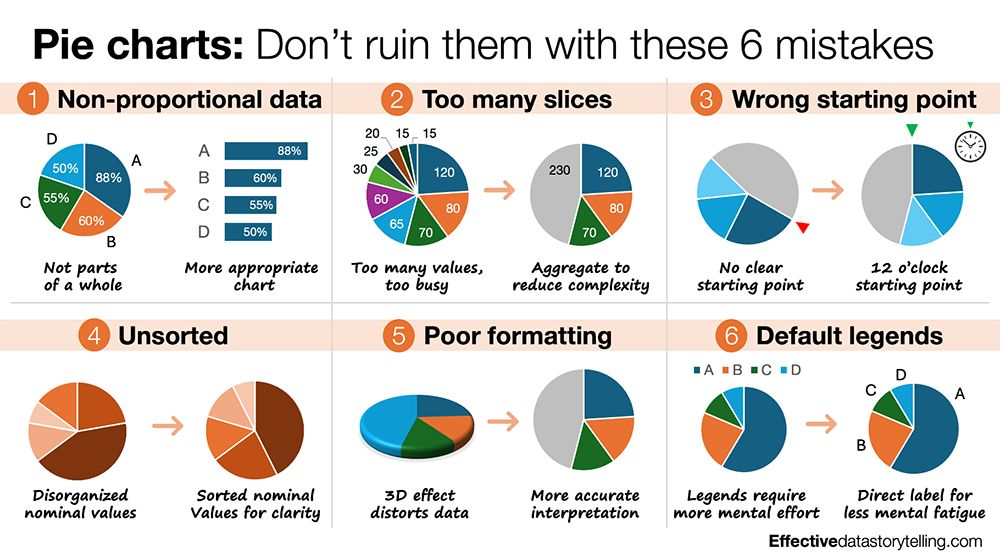
\includegraphics[width=\textwidth]{pie_charts.jpeg}}
\only<15>{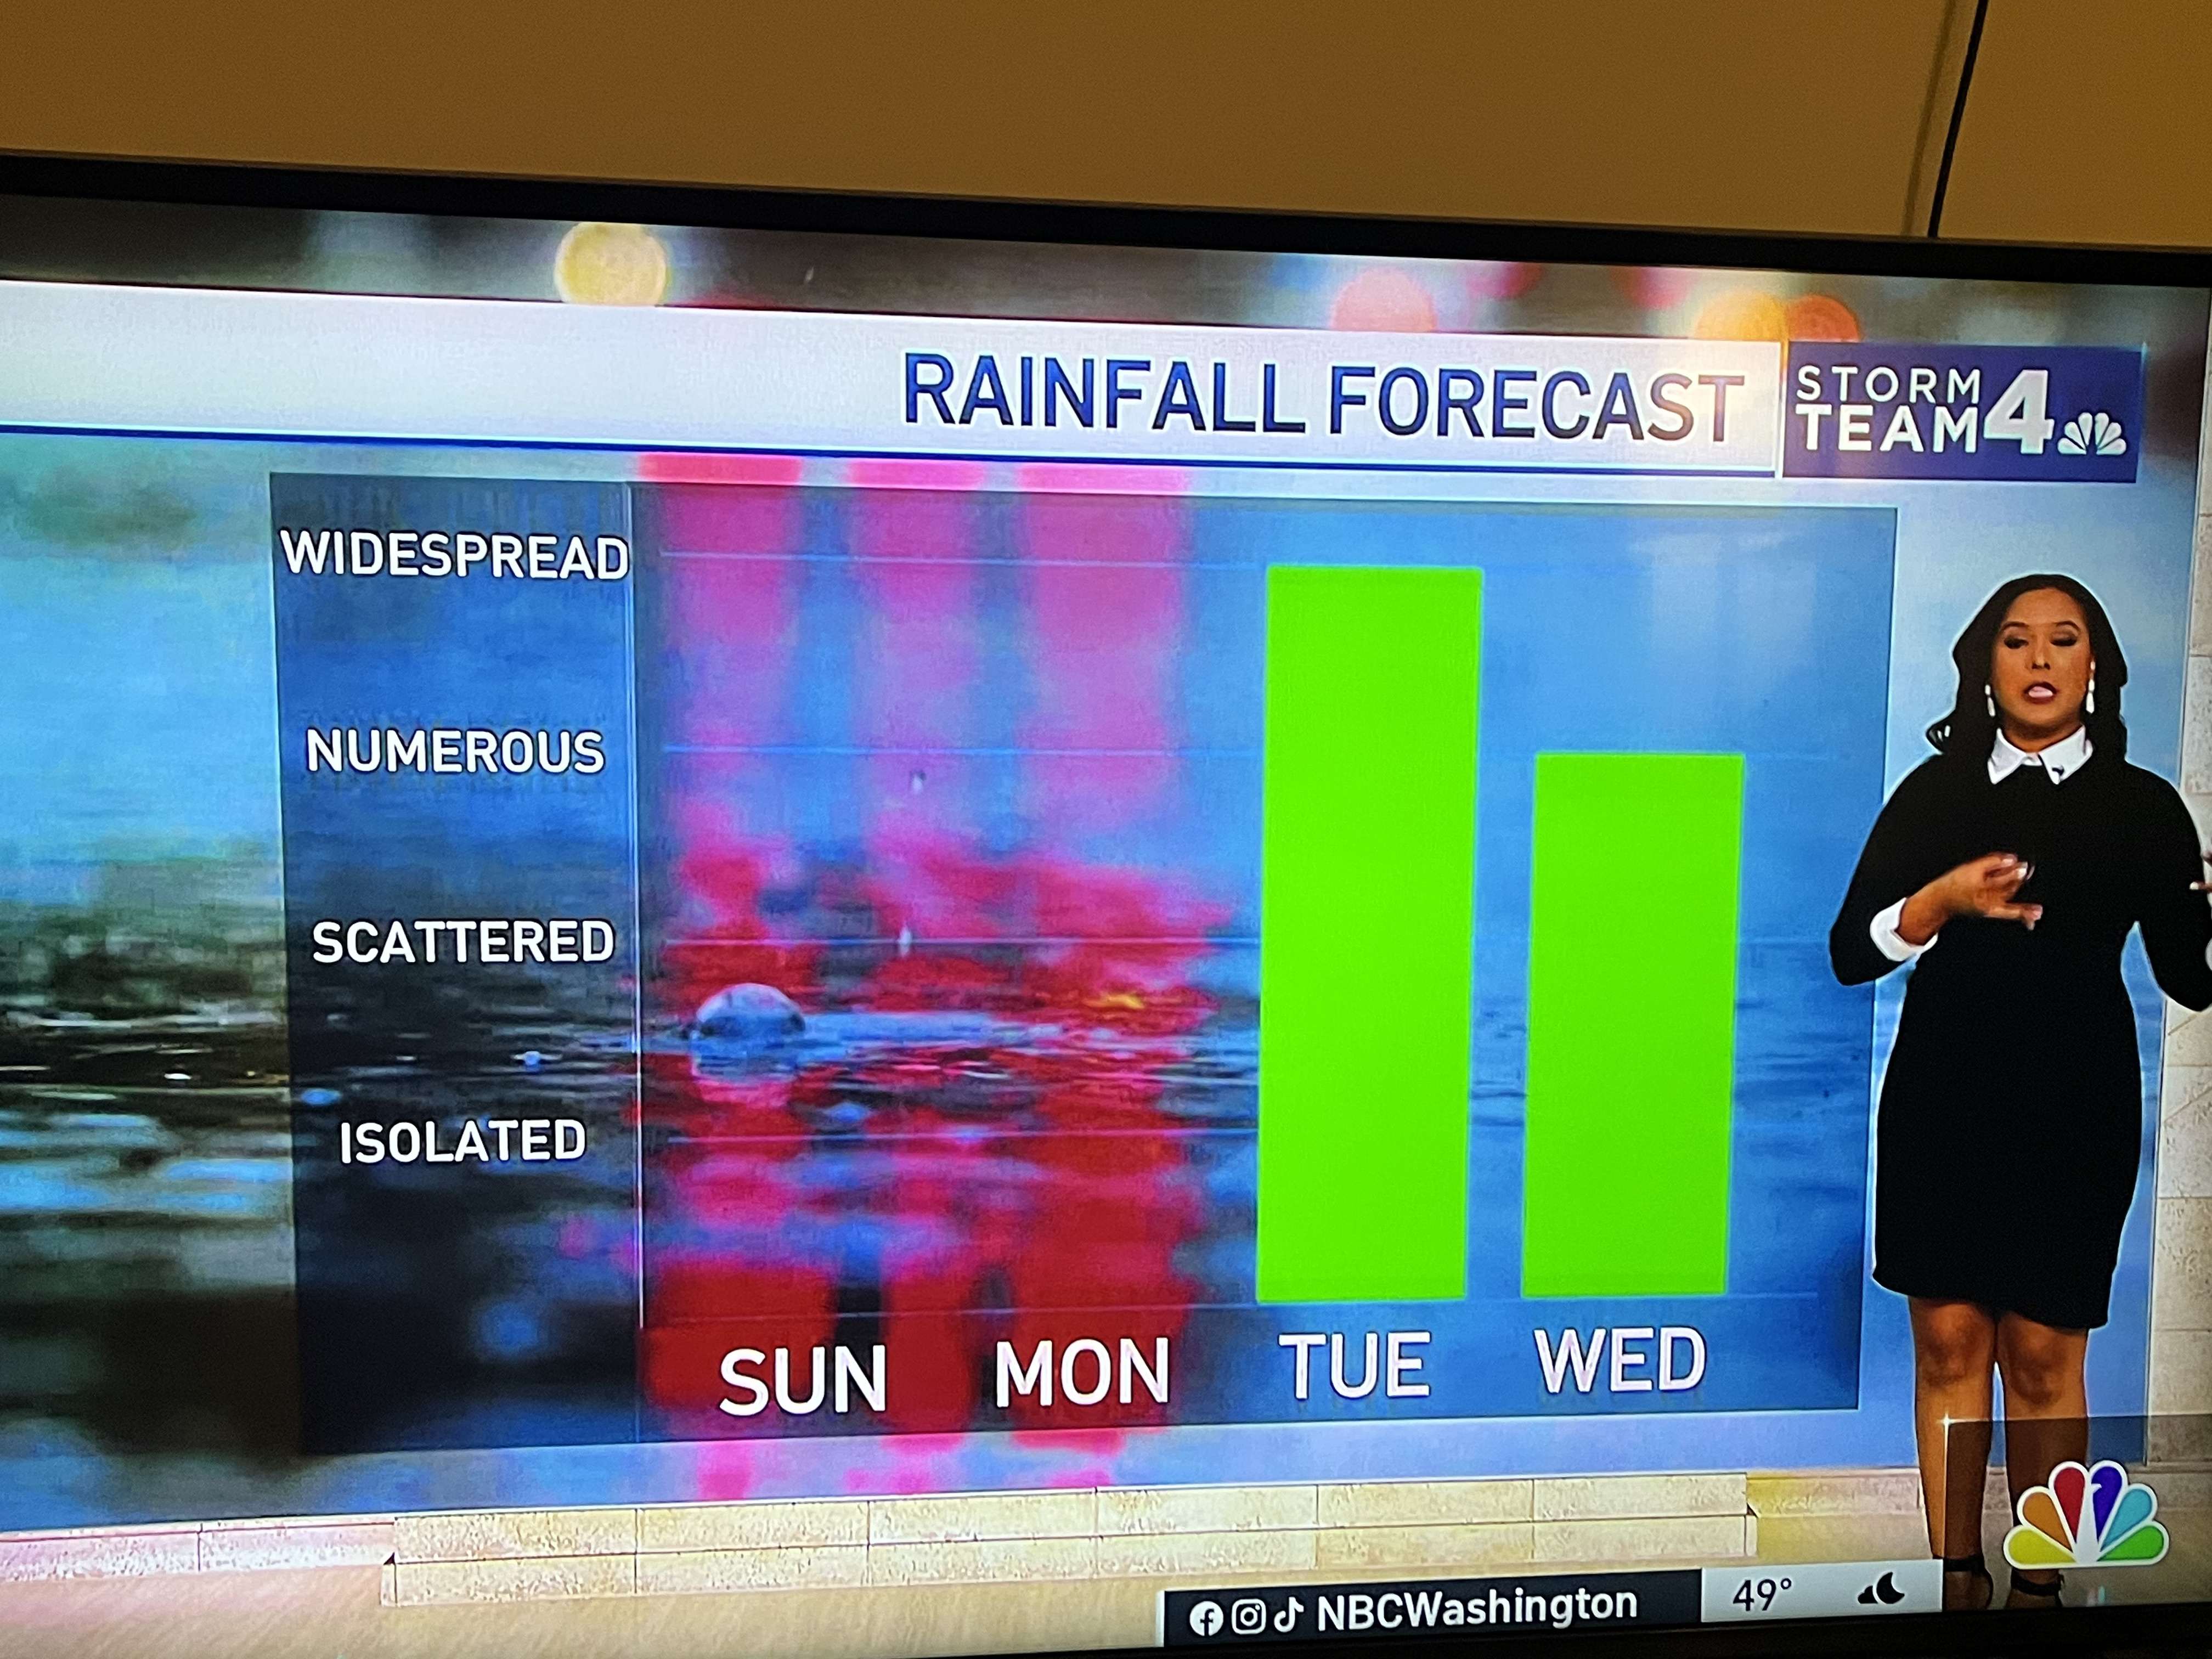
\includegraphics[width=\textwidth]{nbc4_rain.jpg}}
\only<16>{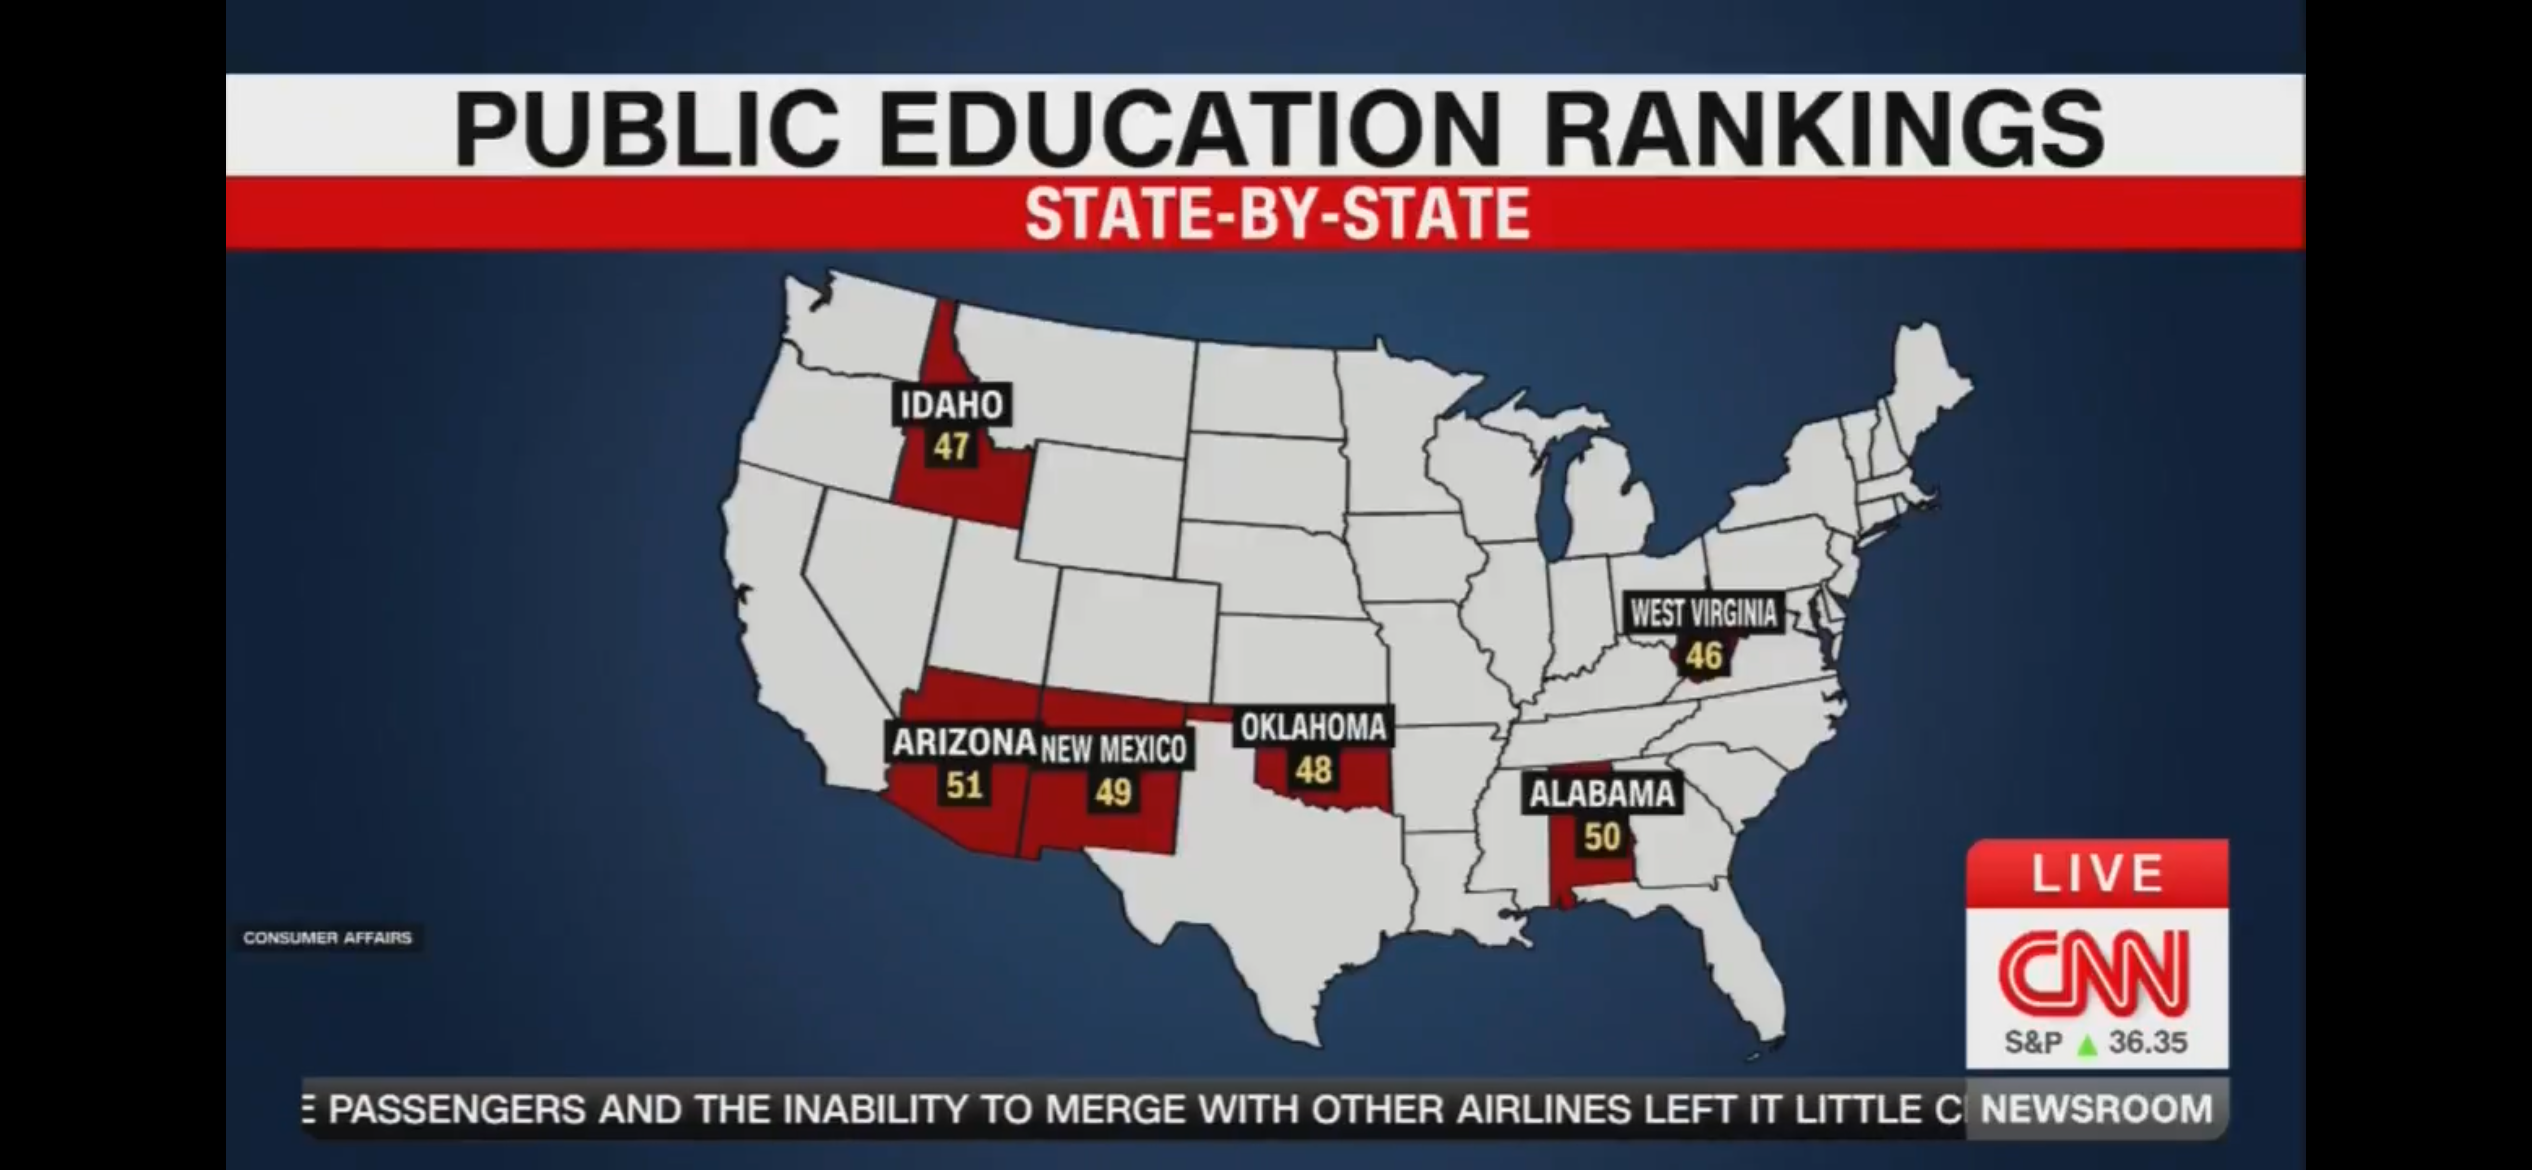
\includegraphics[width=\textwidth]{education_map.png}}
\end{columns}
}

%%%%%%%%%%%%%%%%%%%%%%%%%%%%%%%%%%%%%%%%%%%%%%%%%%%%%%%%%%%%%%%%%%
\frame{\frametitle{Evaluating a Graph}
\begin{columns}
\column{0.4\textwidth}
\begin{enumerate}
    \item Make a note of the first few things you see
    \item Make a note of the first idea that forms in your mind and then search for more
    \item Make notes on likes, dislikes, and wish-I-saws
    \item Find three things you'd change and briefly say why
\end{enumerate}
\column{0.5\textwidth}
\centering
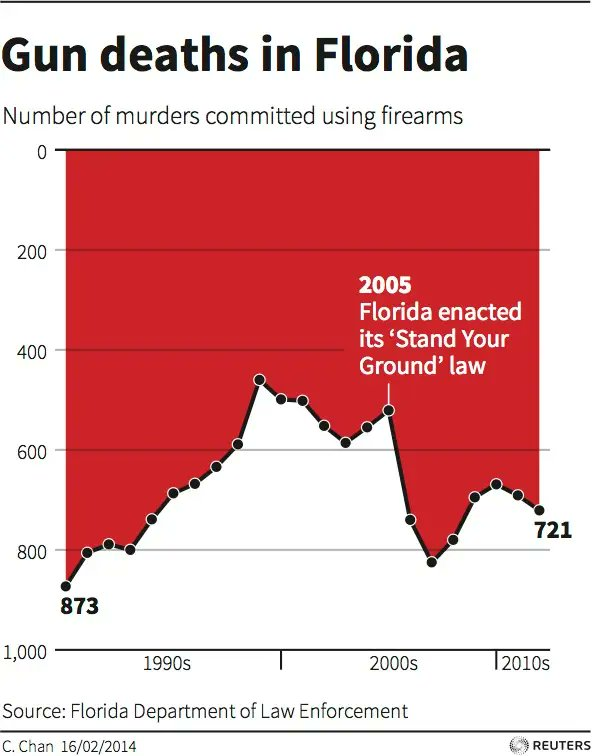
\includegraphics[width=\textwidth]{reuters_guns.JPG}
\end{columns}
}

%%%%%%%%%%%%%%%%%%%%%%%%%%%%%%%%%%%%%%%%%%%%%%%%%%%%%%%%%%%%%%%%%%
\frame{\frametitle{Discussion\\``When Charts Are a Matter of Life and Death''}
\begin{block}{}
    \centering
    ``Data visualization has progressed from a means of making things tractable and comprehensible on the page to an automated hunt for clusters and connections, with trained machines to do the searching. Patterns still emerge and drive our understanding of the world forward, even if they are no longer visible to the human eye.''
\end{block}
}

\end{document}
